% Stanford University PhD thesis style -- modifications to the report style
% This is unofficial so you should always double check against the
% Registrar's office rules
% See http://library.stanford.edu/research/bibliography-management/latex-and-bibtex
% 
% Example of use below
% See the suthesis-2e.sty file for documentation
%

\documentclass{report}
\usepackage{lmodern}
\usepackage{enumerate}
\usepackage{amssymb,amsmath}
\usepackage{ifxetex,ifluatex}
\usepackage{fixltx2e} % provides \textsubscript
\usepackage{hyperref}
\usepackage{longtable,booktabs}
\usepackage{graphicx,grffile}
\ifnum 0\ifxetex 1\fi\ifluatex 1\fi=0 % if pdftex
  \usepackage[T1]{fontenc}
  \usepackage[utf8]{inputenc}
\else % if luatex or xelatex
  \ifxetex
    \usepackage{mathspec}
  \else
    \usepackage{fontspec}
  \fi
  \defaultfontfeatures{Ligatures=TeX,Scale=MatchLowercase}
  \newcommand{\euro}{€}
\fi
\usepackage{microtype}
\usepackage{suthesis-2e}
\usepackage[sort, numbers]{natbib}
\setcitestyle{square}
\dept{Biomedical Informatics}

\begin{document}
\title{Convergent Methods\\
            for Spatial and Semantic Image Comparison}
\author{Vanessa Sochat}
\principaladviser{Russell Poldrack}
\firstreader{Daniel Rubin}
\secondreader{Ruth O'Hara}
\onlinetrue
 
\beforepreface
\prefacesection{Preface}
We can imagine a single statistical result as an effort to capture a
scene. Early master painters, if we might say their efforts were to
reproduce such a scene, were put out of work with the advent of the
photograph. A photographer who develops film was replaced by the
printer, and then digital photography exploded~each single print to
hundreds or thousands of digits. We are now in an era defined by
scientific breakthrough, and the master painters are the scientists
trying to capture the human condition.

For decades, it was acceptable to capture such scenes, and write about
findings with words and pictures. This practice will never scale to keep
up with production rate of these artists, and further, we now have a
small mountain of paintings that must somehow be synthesized into a
coherent, holistic picture. This is not to say that we should change our
expectations for the quality of the work, or to instill rigid layout
specifications to limit the creativity of the artist. We must figure out
how to produce, understand, and archive such results with the quality
and flexibility that we desire en-masse. And just like the photograph,
the answer is not in the content of the paintings, but in the technology
to derive and understand them. In the academic halls of fame,
infrastructure and method have taken a back seat to biological
discovery, until it now is clear that biological discovery will not move
forward without the proper infrastructure and methods in place. I cannot
say that it is not valuable to ask good biological questions, but I am
driven to build tools. If we want reproducible science, and continued
discovery, the academic software developer must assert himself and his
work. Toward this goal I have solidified my passion, and am driven to
provide example and leadership in informatics. I will devote the rest of
my life toward this goal.

This dissertation is a subset of work I completed to complete my
graduate training in the Biomedical Informatics program at Stanford
Medical School. My contributions span both biomedical and informatics,
meaning that I have derived not only methodology that dually supports
our understanding of the human brain, but infrastructure to support it.

\prefacesection{Abstract}

Mental illness encompasses a broad range of disorders that fill the lives of their sufferers with penetrating darkness. In the year 2014 it was estimated that 18.1 \% of U.S. adults experienced a mental illness in the past year \cite{Samhsa_undated-fo}, an alarming prevalence that has allowed mental illness to account for the highest percentage of disability adjusted life years globally \cite{noauthor_2010-wr}. Our current definition of mental illness stems from the Diagnostic and Statistical Manual (DSM), currently in its fifth edition \cite{american2013diagnostic}, and while a behavioral description of disorder is highly useful for clinical diagnosis, unfortunately the disorder groups defined by the manual do not map onto biology \cite{Cuthbert2013-ks}.

In order to address this mental health crisis, researchers would need data-driven, biologically-oriented metrics associated with specific aberrant behavior and cognition. Toward this goal, the National Institute of Mental Health (NIMH) founded the Research Domain Criteria (RDoC) in 2009 \cite{Insel2009-vi}. This initiative would provide impetus for researchers to discover dimensions of genetic, neural, and behavioral features underlying neuropsychiatric disorder and mental illness. The RDoC initiative defines seven domains under which these different features can be studied, including cognition, social processes, arousal and regulatory systems, along with negative and positive valence systems \cite{Morris2012-hx}. This approach places an emphasis on linking core cognitive and developmental processes to behavior and symptoms, holding promise to redefine our definitions for mental illness to inspire better detection and prevention. It follows, then, that filling in this matrix calls for approaches to link cognitive processes to behavior.

Our understanding of human cognition comes from approaches that can measure biological and cognitive variables during the live experience of one or more behaviors. Given these criteria, the primary avenue for understanding human cognition has come from non-invasive brain imaging. We rely on functional magnetic resonance imaging (fMRI) to non-invasively study the human brain across development, during the experience of different cognitive and behavioral tasks, and between different DSM-defined behavior groups. However, neuroimaging technology, supplemented by expertise in cognitive neuroscience, has been around for over two decades. Why, then, has cognitive neuroscience failed to characterize mental illness?

A painful epiphany has been that~more attention has not been given to studying what it means, computationally, to reproduce a
result \cite{Open_Science_Collaboration2015-hb}. Our ability to synthesize the compendium of research in cognitive neuroscience relies primarily on meta analysis. Meta analysis across large datasets can provide validation of the existence of functional brain networks linked to cognitive processes, consensus about how different brain regions contribute to behavioral experience, and can lead to discovery of patterns that are not revealed among the noise of smaller datasets. Thus, while we have confidence that cognitive neuroscience has promise to better characterize mental illness, achieving this goal will require more standardization and best practices for synthesizing results, which come in the form of whole-brain statistical maps that reflect one or more cognitive processes of interest. Simply put, we must have informed ways to link cognitive processes and behavior to our measurement of it with functional brain imaging.  One approach is to utilize the linguistic terms that describe these cognitive processes and the tasks that measure them (represented in an ontology), and then provide the infrastructure and means to annotate statistical brain maps with these terms. Using this annotation, we can then generate "encoding" models to predict entire statistical brain maps from terms alone.  

The responsibility to understand how similar one statistical brain map is to another, a procedure we might call ``image comparison,'' along with the task of properly mapping cognitive processes to our modality to measure them (fMRI) can be helped by Informatics.  Informatics is a subset of science that focuses on the infrastructure and methodology of a scientific discipline. Identifying informed methods to assess the similarity of statistical brain maps, the most basic unit of output for neuroimaging scientists, is a logical first step toward helping cognitive neuroscience. This need to understand best practices and explore different strategies for image comparison motivates the work outlined in this thesis. My goal is to not only study methods, but to provide tools and infrastructure to compare brain images to drive meta analysis and relate cognitive processes to statistical brain maps. My approach consists of: 1) optimizing image comparison to assess the similarity of statistical brain maps based on spatial transformations, and 2) establishing novel semantic methods to drive image comparison based on cognitive processes. 

This second point is a valuable component of this work because it is currently not understood if the terminologies that are used in the field to represent different cognitive processes can be valuable in a classification framework. We define "valuable" as being comparable to a calculation of spatial similarity, a commonly done procedure. For each of these steps, I develop tools and infrastructure to immediately deploy relevant methods and empower researchers to compare their brain maps, and link fMRI to cognitive processes. Such an approach will link behaviors and cognition to specific neural pathways, allowing for a dimensional definition of these processes in the relevant domains of the RDoC matrix. A robust, automated derivation of a metric for fMRI image similarity based on these semantic annotations will be a novel contribution to this field. 

I will first show that there are optimal methods for spatial comparison of whole-brain statistical maps, the first fundamental step of any meta-analysis. I identify pairwise comparison methods that are in line with the goals of the researcher - optimal retrieval of maps from a particular experimental paradigm. This simple method of deriving a similarity score from a thresholded image, and only comparing spatial locations defined in both maps, results in 98.4\% classification accuracy, and is robust across data derived from different individuals and a wide array of experimental paradigms. This work sets up a best practice for individual neuroimaging researchers to find ``brain maps like mine,'' and an informed basis for developers of tools that assess the reproducibility of neuroimaging results based on spatial information.

Next, I present work to suggest that semantic information about the cognitive tasks that give rise to statistical brain maps can be useful in a classification framework. This finding demonstrates that semantic image comparison is useful for image classification, a simple function that is useful in many frameworks that require automated image labeling, and organization. Given this finding, I suggest that semantic classification should be further developed for statistical brain maps, as it offers a much computationally simpler comparison simply by way of the smaller data size. In this work, I will review automated and openly available methods for semantic classification of statistical brain maps, and demonstrate that such a comparison is comparable to the more commonly done calculation of spatial similarity. Adding a semantic dimension, meaning ascribing terms like ``positive feedback'' and ``working memory'' to an image comparison task is essential for several reasons. First, it brings a level of human interpretation to this framework. Second, ontology development is a continually developing science, and it is important to understand if effort in this domain is supported by the neuroimaging data that the ontologies describe. Finally, adding a semantic dimension to image comparison means that brain images derived from novel task structure can be interpreted, a procedure called ``decoding'' that holds promise to predict the cognitive concepts associated with any ``unknown'' brain map.

As a supplement to this work, I include in this dissertation related work for standardization of experimental paradigms used to measure behavior associated with an fMRI protocol (Appendix A), along with a novel tool to visualize these functional networks (Appendix B). Finally, I will bring infrastructure and methods together, discussing best practices and additional tools that I have developed during my
graduate career to empower neuroscience researchers to assess the
reproducibility of their work, and derive new reproducible products (Appendix C). This body of work, including tools and methods for image comparison and reproducible neuroscience, provides compelling example of both the strengths and challenges of
the rising of informatics into the practice of reproducible neuroscience. Cognitive neuroscience will not move forward quickly enough as a science, bringing
with it badly needed intervention for mental illness, if our researchers
do not have better tools. The work outlined in this thesis focuses on
that goal, and is the first of its type to span medical imaging
expertise, machine learning and data visualization, as well as academic
software development.

\prefacesection{Acknowledgments}
I had a challenging early start to graduate school. I started on a path
of trying to fit my research into the aims of others, feeling rushed to
meet milestones and painfully aware of losing touch with the aspects of
research that brought me there in the first place. It was a life
changing event when Russell Poldrack brought his lab to Stanford in the
Fall of 2014. For the first time I was immersed in my field, learning
enormous things from the people around me, and part of a larger, shared
vision. Thus, I am eternally grateful to my advisor, Russ Poldrack, for
supporting me, connecting me with my niche, and providing a rich
environment for me to flourish. I am grateful to Chris Gorgolewski for
showing me an example of prowess in methods, software development, and
sheer attention to detail. I had never before encountered a group that
supported and found great value in my drive to build tools similar to
mine, and this helped me to gain confidence in my own vision for how I
wanted to be. I am grateful to my labmates Sanmi Koyejo, Craig Moodie,
Ian Eisenberg, Patrick Bissett, Mac Shine, Zeynep Enkavi, and Joke
Durnez for their support, humor, and advice. I found everything that I
had always wanted in Poldrack Lab, and it has given me the foundation to
be a better problem solver, communicator, and overall researcher. With
such a foundation, there is no feat I am afraid to pursue, and I am
ready to aggressively pursue building the applications that I've only
dreamed of, continually push myself into challenges and learning new
things, and contribute meaningfully to science.

\afterpreface

\chapter{Introduction}

\section{Understanding brain health}

Brain health is a general idea to describe of how memory, decision making, and other cognitive processes change over time. Brain health is important to study because of its implications for mental health, which broadly describes an individual's well-being. Unfortunately, all is not well.
Mental health has reached a crisis state in the United States, with the
cost of ``severely debilitating'' disorders alone accruing to a total of
\$300 billion annually \cite{noauthor_undated-ou}.
These disorders are complex syndromes, with evidence for problems with
brain connectivity \cite{Horwitz2012-ci,Fornito2015-rv}
resulting~from poorly understood interactions between environmental, and
genetic variables \cite{McCarroll2013-hi}
Essential to developing informed intervention for these aberrant
cognitive processes and behaviors is continual growth of our
understanding how environment \cite{DeWit2000-wh}
behavior \cite{Schmidt2007-cs},
and developmental variables \cite{Broman1999-dq,Ten_Donkelaar2014-ps} are
related to brain function, and impetus to redefine these disorders in a space of data-driven, biological metrics. The Research Domain Criteria (RDoC) initiative \cite{Insel2009-vi} established by the National Institute of Mental Health (NIMH) is such a space, including several domains (cognition, social processes, arousal/regulatory systems, negative and positive valence systems), each of which can be described with genetic, neural, and behavioral features. While each domain has potential value to redefine definitions of disorders, compelling research has shown a strong link between cognition and mental health \cite{Etkin2013-lo}, and so a data-driven strategy to computationally describe and define cognitive processes would be a significant contribution toward helping solve the mental health crisis.

\subsection{The link between cognition and brain health}
Cognition broadly encompasses the domains of memory, attention, decision making, regulatory behaviors, abstract thinking, and language. For some individuals (an estimated \~18\% of adults in the United States \cite{Samhsa_undated-fo}) problems arising in any of these domains can have a significant negative impact on quality of life. We call these patterns of aberrant processes mental illness, and historically our definition of these patterns has been categorical, defined in a book called the Diagnostic and Statistical Manual of Mental Illness (DSM) \cite{american2013diagnostic}. In spirit of the RDoC initiative, badly needed is a data-driven understanding of how cognitive processes map to behavior, however such an understanding is a chicken and egg problem. Due to observing cognitive deficits in many disorders, it might be a natural strategy to assume that such deficits appear as a result of a disorder. Recent work \cite{Etkin2013-lo} has suggested a new perspective that encourages viewing cognitive function less as a passive symptom, and more as a target for treatment. Aberrant cognitive processes can not only be measured to indicate present disorder, but also can be used to predict the course of an illness, or progress in treatment. Thus, we need cognitive neuroscience to better characterize mental illness.

\subsection{Non-invasive brain imaging as a means to measure cognition}
A majority of knowledge about cognition, specifically the linking between desirable or undesirable behaviors and cognitive processes, comes by way of non-invasive brain imaging. Functional Magnetic Resonance Imaging (fMRI) allows for the measurement of biological and cognitive variables during the live experience of some task paradigm. fMRI has given huge insight to our understanding of brain networks associated with domains of behavior (see \cite{Etkin2013-lo} for a review), however it remains the case that neuroimaging technology supplemented by expertise in cognitive neuroscience, has not yet robustly characterized mental illness. Aside from issues related to power \cite{Button2013-ja} or reproducible practices \cite{Stodden2014-ca,Boettiger2014-cz,noauthor_2014-zc} why might this be the case? Variability in image acquisition protocols \cite{Fera2004-ok}, especially for smaller brain regions \cite{Barry2013-ng}, is an influential factor when assessing the reproducibility of a result. However, metrics such as signal to noise ratio (SNR) are routinely used to provide best practices for advances in technology \cite{Triantafyllou2005-zk}, and educate researches on the protocols \cite{noauthor_undated-nb}. A larger challenge is instilling best practices for the parameters used during image processing (\cite{Norris2006-cs,Turner1998-aj,Secca2008-dn}), and efforts like the Stanford Reproducibility Center for Neuroscience (\href{http://reproducibility.stanford.edu}{http://reproducibility.stanford.edu}) will be able to instill standardization by offering analysis as a service, and by taking a data-driven approach to defining reproducibility. The center can optimize analysis pipelines by running an equivalent dataset through all possible pipelines, and choosing a processing strategy that, for example, maximizes signal to noise, number of activated voxels \cite{Yang1999}, or optimizes another metric of interest. The issue of variability at the level of acquisition has also been helped by large efforts such as the Human Connectome Project (HCP) \cite{Van_Essen2012-wp,Van_Essen2013-fi} that have combined expertise of many neuroimaging scientists to establish robust pipelines that the larger community can exemplify. Finally, it isn't clear that consensus across scanning parameters is ideal. In the field of radiology, for example, there is huge diversity in terms of hardware and protocol, yet radiologists at different institutions are still able to successfully make diagnoses from images independently of the machine used. Arguably, a brain phenomena that is robust (and not noise itself) will emerge despite subtle differences in the acquisition technology.

Arguably, the missing link is a validated connection between patterns of brain activation present in fMRI, and specific cognitive processes. If we could make assertions that particular patterns of brain activation that are understood as functional networks are indicative of particular cognitive processes, it would be possible to measure such networks in individuals with mental illness for purpose of diagnosis or treatment. The first step is a proper definition of the space of cognitive processes, and relationships between them.

\subsection{The Cognitive Atlas}
Understanding of the underlying drivers and influences on behavioral
outcomes usually starts with a specific behavior or cognitive phenomena
of interest. Let's say that we enter a cafe, and enter an interesting
conversation with a behavioral researcher. As he describes how some
people have aberrant behavior related to decision making, the researcher
might use terms such as ``impulsivity,'' ``choice,'' or ``risk,'' when
describing his hypotheses about how integration of different cognitive
processes can lead to something that looks like ``decision making.'' In
fact, he has designed an experiment to measure his phenomena of
interest. Given the success of his experiment, how might we categorize
the resulting data if we, at some point in the future, wanted to do a
large-scale meta-analysis about decision making? It should be
immediately clear that if we do not have a standard terminology for
describing different cognitive paradigms, their conditions, and the
cognitive processes measured, we will not be able to make any inferences
with semantic features like ``choice'' and ``risk'' that are directly
relevant to the cognitive processes that we wish to study.

The Cognitive Atlas \cite{Poldrack2011-jp} is
an effort to represent, formally, concepts in cognitive science. It can
represent, in a standardized way, different experimental paradigms and
cognitive processes. An analogy can be made to the better known Gene
Ontology (GO), an ontology that has driven discovery in biology by
mapping all gene products into three domains, including cellular
components, molecular components, or biological processes \cite{Ashburner2000-am}.
In the same way that we can derive that ``regulation of collagen
binding'' and ``regulation of receptor binding'' are similar in that
they share a common parent of ``regulation of protein binding,'' by
knowing that ``inhibition'' and ``updating'' are kinds of ``cognitive
control,'' we can use these relationships to drive discovery in
cognitive science. By mapping these terms ``inhibition'' and
``updating'' into the Cognitive Atlas, we can discover the parent term
of ``cognitive control'' and integrate this relationship into an
analysis that might have otherwise treated brain maps with these
``different'' labels as entirely different things. The open source and
public nature of the ontology means that future researchers can use and
critique terms, and better refine our understanding of concepts in
cognitive science. 

This approach does not come without challenges. Development of the ontology itself is an arduous process that requires substantial expertise, and is prone to disagreement. Ideally, defining relationships between terms would be done programmatically with careful steps such as validation done via manual intervention. Arguably, cognitive neuroscience has not made substantial advancement to lead to development of a modern vocabulary (Poldrack, Duke University April 2016), and it isn't clear if the terms typically used in manuscripts (e.g., working memory, decision making, risk seeking) represent the field's best effort. Quality of definitions may not be consistent across terms, and so work would be needed to assess the validity of the terms. Finally, definition of terms is not enough to build the ontology, as relationships between terms must be identified as well. Despite these limitations, a standard description such as the Cognitive Atlas is an essential component to a framework that aims to measure cognitive processes.

\section{Interpretation of~neuroimaging results to synthesize our understanding}
Functional brain imaging, as was previously stated, is the primary avenue to non-invasively study
human brain function that leads to behavior. Thus, understanding the basis of aberrant behavior to help the mental health crisis is
contingent upon synthesizing the compendium of neuroimaging work to make
associations between functional brain networks and cognitive processes.
This synthesis is the first action when the neuroimaging scientist
obtains a new result, a statistical brain map with effect sizes that
reflect a cognitive process of interest. The goals of the researcher in
this process are many:

\begin{itemize}
\item
  use results from different studies to better understand a question of
  interest
\item
  accumulate evidence to gain statistical power
\item
  determine the association of a brain region to a task of interest
  (reverse inference)
\item
  assess the probability or likelihood of a new result based on previous
  ones
\end{itemize}

If a single result is simply a three dimensional matrix of numbers, the
above tasks can be understood as a ``statistical pooling of
information'' \cite{Lazar2002-dk}.
In fact, this is done on many levels in neuroimaging science. When we
want to understand how a group of individuals with some phenotype may be
different in their brain function~from another group, we ``pool''
individual brain maps into a group map to make higher level inferences \cite{Smith2004-lw}.
When we want to compare across studies, we then ``pool'' these group
maps to perform meta-analysis \cite{Costafreda2009-ys}. Unfortunately, the way that these comparisons has been historically done is reflective of the data that was available at the time, which was a subset of x,y,z coordinates extracted from the statistical maps into tabular formats for publication. We call these meta-analytical approaches that use coordinates "coordinate-based," and this is in contrast to using whole-brain statistical maps in an analysis, called a "voxel-wise" approach. The lack of developed methods for voxel-wise statistical brain maps is the primary motivation of the first component of this work. The transition from coordinate-based data to voxel-wise data can be thought of as a tradeoff between resolution of the meta-analysis. To best understand this tradeoff and the influence it has on the interpretability of the result, we will first review the two approaches: coordinate-based and voxel-wise meta-analysis.

\subsection{Coordinate and voxelwise approaches to compare images}

This simple task of image comparison has flexibly adapted to match the
availability of data. There are two general approaches: coordinate-based
meta analysis (CBMA), and image-based meta-analysis (IBMA).~A brain map
is a three dimensional matrix of numbers, where each x,y,z coordinate in
this space, called a ``voxel'' might hold a value that represents the
result of a statistical test of interest for that location. To
standardize this coordinate space, the neuroimaging community has
developed several standard ``coordinate spaces,'' including Talaraich
and MNI, the first being developed from a single individual \cite{Talairach1988-os},
and the latter a more proper probabilistic atlas derived from hundreds
of individuals \cite{Mazziotta1995-gn,Brett2001-gk}.
Having these standard coordinates led to the reporting of results in
papers by way of tables of coordinates (an example is provided in Figure~\ref{fig:11}), with detail added about the coordinate being in Talaraich or MNI
space.

\begin{figure}[ht!]
\begin{center}
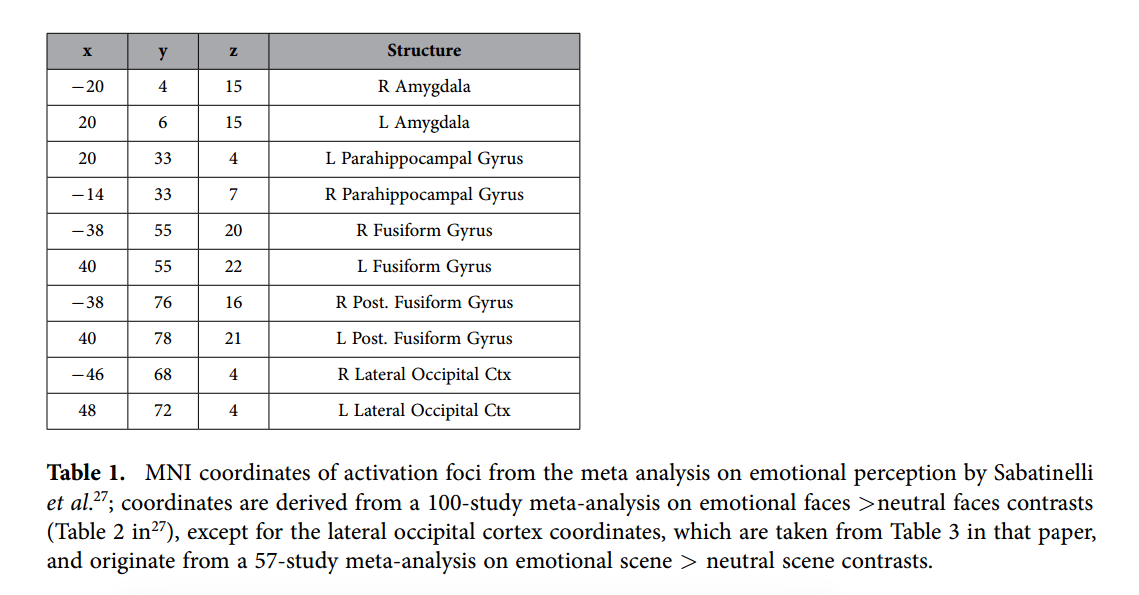
\includegraphics[width=15cm]{images/figure11.png}
\end{center}
\caption{\label{fig:11} Coordinate Reporting: coordinates in the MNI or Talaraich standard brain spaces are typically reported in a tabular format in manuscripts \cite{Boubela2015-ap}.}
\end{figure}

Back in the early days when finding these ``voxelwise'' statistical map
results on the internet was a rarity, synthesizing results meant parsing
these standardized coordinates from the papers to find commonality of
results. A coordinated effort to do this led to the development of the
BrainMap database \cite{Laird2005-gm},
a resource that has allowed for more than 500 publications at the time
of writing this dissertation. Tools such as GingerALE \cite{Brown2005-sb} to
deploy a method called ``activation likelihood estimation'' \cite{Eickhoff2012-iw}
then empowered researchers to manually enter significant coordinates across
studies to summarize a set of interest.~The requirement for manual entry
of these results called for more automated approaches, and the
pioneering NeuroSynth \cite{Yarkoni2011-rg} made
this possible. The NeuroSynth database is a publicly available
collection of coordinates that are automatically parsed from online
neuroimaging literature. ~While BrainMap covers just over 2,700 papers,
NeuroSynth has expanded to cover over 13,000 in only five years. Given
this expansive set of data, what methods are available to synthesize it?

\subsubsection{Coordinate Based Meta Analysis (CBMA)}

Generally, CBMA approaches include quantitative analysis of specificity \cite{Pearce1992-nr},
chi-square tests, analysis of reported peak density differences, and
pattern classification \cite{Salimi-Khorshidi2009-if,noauthor_1949-ry,Jackson1979-hc}.
While a quantitative assessment of p-values to perform meta-analysis is
useful for many domains of research \cite{Pearce1992-nr}, these
methods proceed without the benefit of a key source of information, the
spatial maps themselves. I will first review CBMA methods, followed by
IBMA. I will discuss the caveats of these approaches, and how we must
transition to a large-data, reproducible image comparison framework.

\paragraph{Analysis of Reported Peak Density Differences}

These approaches generally~map coordinate results~into a standard brain
space to find areas of significant overlap~with higher values, called
``peaks.'' These faux-maps are treated as representations of the
original spatial maps from which they were derived. A typical method
might count peak activations in each voxel, convolve the resulting
histogram with a kernel (e.g., sphere or Gaussian), and compare the
result to some null distribution. The null hypothesis is that the
distribution of peaks is randomly and uniformly distributed. Thus, if
the same general method is performed with randomly placed points, this
forms our null distribution for comparison. A method such as Monte Carlo
simulation might be used to calculate a p-value, and assess the
significance of the difference between the result and the null \cite{Salimi-Khorshidi2009-if}.
Specific implementations of this process are derivations of this general
approach, using different kernels and final metrics for comparing the
null to the result.

\subparagraph{Kernel Density Analysis (KDA)}

In KDA, the smoothing kernel applied to the data is spherical, typically
with a radius of 10-15mm. A value in a KDA map can be understood as the
number of peaks within a radius of some R millimeters away from the
spatial location. These maps can be divided by the volume of the kernel
to derive a density in peaks per cubic millimeters. For KDA, we perform
the procedure with randomly placed points, and compare the top density
value from the random points to our actual data \cite{Salimi-Khorshidi2009-if}.

\subparagraph{Activation Likelihood Estimation (ALE)}

The ALE approach uses a Gaussian kernel, with width specified by a full
width half maximum (FWHM) value, such as 10 millimeters. In the ALE
approach, a smoothed value in the map can be understood as probabilities
of each peak being within some R millimeters from the spatial location.
The union of these values is computed to derive the activation
likelihood, the score of interest that is an estimate of at least one
peak activation being within the spatial location (``voxel'') of
interest. Assessment of significance means identifying the voxels where
the union of probabilities is greater than chance probability.

\subparagraph{Multi-level Kernel Density Analysis (MKDA)}

In the MKDA approach, a single unit of analysis is a contrast map from a
study.~The same procedure is done as outlined previously, however
instead of generating maps that reflect the frequency of activations,
the output is a binary ``contrast indicator'' map (a value of 1
indicates a peak within a radius of some R millileters from a spatial
location, and 0 not) that can be weighted by a metric relative to the
study to produce a density map, For example, the indicator maps could be
weighted by study quality and sample size to get a density map. The null
hypothesis is that the distribution of peaks within each contrast
indicator map is randomly distributed, however the MKDA approach places
entire clusters (and not random points). A significant result then can
be understood as finding some proportion of the indicator map being
consistently activated within R millimeters at a rate greater than
expected by chance \cite{Salimi-Khorshidi2009-if}.
The benefit of MKDA is that it can be used to compare two conditions,
meaning doing the process separately with two different data sets, and
saving maximum values for the differences between the maps at each
iteration of Monte Carlo simulation. MKDA also improves upon ALE and KDA
in that it has been shown empirically to better control false positives.
Thresholding on the distribution of saved differences then creates a
difference map. However, the results of these difference maps don't say
anything about activation in the regions being associated with either of
the contrasts, calling for a chi-squared approach.

\subparagraph{Chi-Squared: NeuroSynth}

The chi-squared approach allows for comparison of observed activation
frequencies against a null hypothesis. The best deployed example is via
the NeuroSynth database. NeuroSynth collects and organizes voxelwise
coordinate data relevant to brain activity, and measures the
association~between these coordinates and terms from the paper~such as
``anxiety'' or ``memory.'' The automated approach is logical to make the
assumption that a publication related to the experience of ``anxiety''
is likely to have a high frequency of mentions of the term.~The original
NeuroSynth algorithm, for each spatial location in the human brain,
generated a 2x2 contingency table of counts to indicate if activation is
present or absent when a specific behavior term is present or absent.
The current algorithm takes an approach similar to KDA, first convolving
the data with a 6mm sphere to smooth the activations spatially, and then
generating counts from this map. A Chi-Square test of independence is
then used to determine if there is a significant dependence between the
term and activation, and p-values are false discovery rate
(FDR)-adjusted to account for multiple hypothesis testing at a threshold
of 0.05 \cite{Yarkoni2011-rg}. The initial dataset relied upon parsing of full-text, publicly
available manuscripts, and the most recent version
(\href{https://github.com/neurosynth/neurosynth/releases/tag/0.3.3}{https://github.com/neurosynth/neurosynth/releases/tag/0.3.3}) has
transitioned to parsing more readily available abstracts and maintained
the quality of the result.

These approaches make strong assumptions that studies do not differ in
peaks reported, location, smoothness, false positive rates, and
statistical power. Specifically, for ALE and KDA, a single study with
many reports can highly influence the result, and we make the incorrect
assumption that peaks are independent within and across studies until
the null. These approaches yield results with many false positives, and
further, we cannot infer from any of these results that repeating a
study will produce activation in the identified regions. While they have
been useful, these drawbacks call for utilizing the original spatial
maps to drive the meta-analysis.

\subsubsection{Image-based Meta Analysis (IBMA)}

IBMA, in using the whole-brain statistical map, has historically been
treated as a ``gold standard'' for assessing coordinate-based
approaches. In a pioneering study \cite{Salimi-Khorshidi2009-if},
Salimi et al compared the assortment of CBMA approaches (Figure~\ref{fig:12}).

\begin{figure}[ht!]
\begin{center}
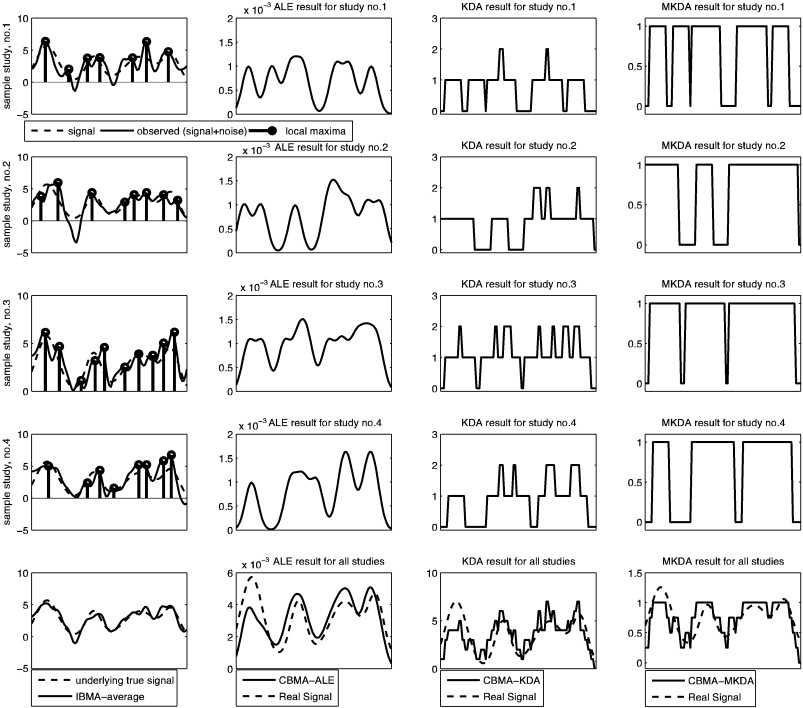
\includegraphics[width=15cm]{images/figure12.jpg}
\end{center}
 \caption{\label{fig:12} Figure 1 from Salimi et. al. illustrates a 4-study, 1-dimensional meta-analysis, demonstrating that even the simplest voxel-based method (IBMA) outperforms all coordinate-based methods. Identifying optimized methods for IBMA is thus a primary goal in this work. The caption of the original figure reads: ``A true signal (dashed line) is created
and four simulated statistic `images' are created by adding smoothed
white noise to the true signal (bold lines in the first column of the
first four rows). To apply CBMA to these simulated 1D studies, local
maxima (foci) are extracted from each observed signal (circles on the
bold lines). Next, the locations of these foci are fed into each CBMA
technique. In the last row, the results of each method in reproducing
the true signal using the foci are shown. As can be seen, averaging over
the complete signals (as IBMA does) yields a better estimate of truth
compared to using local maxima (CBMA).''}
\end{figure}

These plots \cite{Salimi-Khorshidi2009-if} compare
IBMA to each of ALE, KDE, and MKDA. In the first column, the
gold-standard IBMA uses large black dots to show local maxima that are
reported in the whole-brain maps. The second column shows results from
ALE. The result is more of a curve because the ALE statistic reflects a
probability value that at least one peak is within some R millimeters of
each voxel. The third column is KDA, which gives us a value at each
voxel that represents the number of peaks within R millimeters of that
voxel, and dividing by the voxel resolution gives us a ``density.''
Finally, the last column is MKDA, which is the same as KDA, but the
procedure is done for each study, and the resulting ``contrast indicator
maps'' indicate the presence or absence of a peak within some R
millimeters.

Each of these plots uses simulated data. The ``true'' signal is the
dashed line, and the bold lines in the first column of each row are that
signal with added noise. The dots in each plot would be the ``extracted
peak coordinates'' reported in some papers. We can then look at each row
to see how KDA, ALE, and MKDA perform on just the single ``study'' data,
and the last row shows how the methods perform for meta-analysis across
all the studies. The figure shows that the IBMA (averaging over the
images) produces a signal that is closest to the original data, an
improvement over the CBMA approaches. This investigation sets up
compelling evidence that even a simple metric that utilizes the entire
spatial map is an improvement over traditional CBMA approaches, and
encourages the field to move in that direction. In fact, the paper is
quite foretelling:

\textit{``Another promising future direction is the development of
meta-analysis-based classifier techniques that will allow quantitative
inferences to be made from brain activation to psychological states.
~This kind of analysis will allow us to make formal predictions about
psychological states based on brain activation. Another exciting
direction is that analyses across many study types can enable us to
develop brain-based psychological ontologies---that is, to group
different kinds of tasks and psychological functions together based on
the similarity of their brain patterns.''}

This paragraph foreshadows things to come, specifically, the use of
semantic knowledge and databases with whole-brain maps to make
inferences between cognitive paradigm and psychological states. This paper also emphasizes an important point that motivates this work in what is unsaid. There is much emphasis on methods for comparison of coordinate-based data, but only one "average" approach to represent comparison of whole-brain statistical maps.  It isn't clear if a particular metric, or thresholding of the images would be an optimal way to compare whole brain statistical-maps, and this is a foundation of motivation for this dissertation work.

\section{Large Scale Image Comparison}

CBMA approaches were appropriate for a landscape under which we did not
have availability of entire statistical maps.~This is not to say that
one approach is better than the other (in fact coordinate data can be
viewed as a transformation of whole brain data into a reduced
representation), but rather researchers must choose where to operate
along the dimension that spans between a whole brain map and a small set
of coordinates that represent it. Whole brain map data is higher quality
in that it does not strip away valuable information represented in the
non-significant values, however using it comes at the cost of requiring
more computational resources and storage. However, the neuroinformatics
landscape is changing to accommodate these larger data. Databases such
as NeuroVault \cite{Gorgolewski2015-gu}, ANIMA \cite{Reid2015-gt},
NDAR \cite{Hall2012-qo}, the Human Connectome Project \cite{Van_Essen2013-fi},
and others \cite{Book2016-ro,Landis2016-wo}, are delivering whole-brain
statistical maps~for the research community. Notably for databases like
NeuroVault for which a researcher can share a map that does not have a
``significant'' result (as publication of these results is highly
challenging), we are able to start addressing the problem of publication
bias in meta-analysis.

However, under the assumption that we have collected a set of brain maps
that we want to compare, it is not a trivial task to decide how to do
this. We may want a ``pair-wise'' comparison, meaning to take a single
group result and derive some similarity score to all other group
results, or we may want a holistic summary, meaning a single brain map
that somehow combines across group maps. The simplest IBMA approach
would be to take an average over a set of images, but such an approach
would likely smooth away signal, and information about variance across
studies. The problem of performing image-based meta-analysis comes in
two parts: the development of robust metrics to integrate information
such as effect size and variance, and higher level strategies to perform
the IBMA across disparate data sets. A reasonable first goal, and the
motivation behind this work, is to understand how different
transformations of brain maps, and different kinds of high level
features, contribute to an image comparison. Further, the goals of the
image comparison must be taken into account, meaning identifying maps
that were derived from studies of interest. We can think of this
labeling of studies in two different feature spaces, semantic and
spatial.

\subsection{Spatial and semantic understanding}

The analysis of images brings with it a complex feature space, as an
image can be understood not only in terms of its pixel or voxel values,
but also in terms of more complex derived features and knowledge-based
annotations. For this work, I will refer to features based on
description of the values themselves as ``spatial,'' and features
associated with terms to describe the images as ``semantic.'' While the
large majority of work (for example, the methods previously described)
derive comparisons based on spatial features, evidence suggests that
there is value in both semantic and spatial features \cite{Sochat2014-wz}
to classify images. Semantic understanding is important because as human
beings reliant on language, it is with terms that we describe behavioral
paradigms and cognitive processes. We do not intuitively understand a
phenomena such as ``decision making'' as numerical values associated
with peak coordinate locations and activations, but rather as a
collection of semantic terms that we hypothesize describe this complex
cognitive process. As a result, we have developed ontologies, or
descriptions of entities and the relationships between those entities,
for cognitive processes. It is by way of associating these standard
terminologies with whole brain statistical maps that we can make
statements or inferences about the function of the human brain in terms
that humans can actually understand.

\section{Informed Image Comparison}

To move forward, we must be able to develop methods for informed comparison of brain
maps that result from these experiments. This means a collaborative
process of developing, deploying, and making assertions about the
cognitive concepts that an experiment aims to measure, followed up with
discussion and validation of those assertions in the data being
collected. Success in this process calls for convergence in the
methods used to compare images, integration with standard
terminologies, and robust annotation of data associated with
experiments. However, before we can invest in this approach, we must be
confident that making any such assertions is useful to meet the goals of
the researcher attempting to synthesize what we understand about the
human brain. Specifically, this approach must add value to performing a
meta-analysis over functional neuroimaging data. Unfortunately, best
practices for spatial comparison of images, let alone semantic
comparison using standard terminology associated with particular
experiments, is poorly studied. Ideally, these two feature spaces would
be in agreement, and we could better harness both spatial and semantic
features to make inferences about the cognitive processes underlying
behaviors that emerge from the human brain.

\section{Specific Aims}
It is clear that the neuroinformatics landscape is growing in the
availability of whole-brain statistical maps for meta-analysis, as well
as terminologies to describe them, but lacking in publicly available software with robust methods to perform meta-analysis across disparate resources. Toward the goal of
developing convergent methods for image comparison, the specific aims of my dissertation were:

\begin{itemize}
\item
  Aim 1: to define optimized, spatial pairwise image comparison
  strategies
\end{itemize}

\begin{itemize}
\item
  Aim 2: to assess semantic image comparison against traditional
  approaches
\end{itemize}

In Chapter 2 (Aim 1: Spatial Image Comparison) I will show that there
are optimal methods for spatial comparison of of whole-brain statistical
maps. I identify pairwise comparison methods that are in line with the
goals of the researcher - optimal retrieval of maps from a particular
experimental paradigm. This simple method of deriving a similarity score
from a thresholded image, and only comparing spatial locations defined
in both maps, results in 98.4\% classification accuracy, and is robust
across data derived from different individuals and a wide array of
experimental paradigms. This work sets up a best practice for individual
neuroimaging researchers to perform meta-analysis, calculate similarity
of brain maps for purposes of determining replication, and an informed
basis for developers of tools that assess the replication of
neuroimaging results based on spatial information.

In Chapter 3 (Aim 2: Semantic Image Comparison) I present work to
suggest that semantic information about statistical brain maps can be
useful in a classification framework. This is essential toward the goal of developing convergent methods for image comparison for three reasons. First, it offers a less computationally intensive comparison metric. Comparing vectors of human-derived labels to describe images has a much smaller dimension than the hundreds of thousands of features that are represented in the spatial dimension. Second, spatial image comparison brings a component of human understanding to image comparison. Knowing that a statistical brain map has higher or lower values at different coordinates is hard to derive meaning from, but knowing that it is most highly matched to terms like "working memory" or "response inhibition" gives a researcher a more interpretable understanding of the data. Finally, semantic image comparison brings the rich world of standard terminology and description of relationships (ontology) to neuroimaging. Researchers can collaborate on these language knowledge bases to better unify and standardize the field. The first step to evaluate the utility of semantic annotations toward image comparison to enable these enhancements is to demonstrate that semantic comparison is comparable to the more commonly done calculation of spatial similarity. I first tackle this, and additionally review the currently available terminologies for describing cognitive processes and tasks. Finally, I fully demonstrate the value of the semantic annotations by showing that I can predict whole brain statistical maps from cognitive concepts alone.

In Appendix A (Standardizing Behavioral Experimentation) I discuss
an applied extension of my work: an open source, infrastructure to
collaboratively develop and deploy behavioral experiments. Standardization on the level of the experimental paradigms themselves is essential to remove variance in the task portion of the study of behavior. I have
created standard data structures, virtual machines, and web-based
software to assist researchers with the definition and generation of
experimental paradigms. This work will further bring reproducibility to
behavioral science.

In Appendix B (Visualization Best Practices for Complex Brain Connectivity Data) and Appendix C (Best Practices for Reproducible Research) I discuss
best practices and technology for reproducible science. To supplement
these points, I provide examples of web-based tools that I have
developed to assist with analysis, retrieval, and visualization. I
provide these tools as publicly available resources for sharing,
viewing, and performing meta analysis for whole-brain statistical maps.

This work, which can be called ``Convergent Methods for Spatial and Semantic Image Comparison'' will be the first of its type to span
medical imaging expertise, machine learning, and data visualization to bring standardization to the image comparison tasks that are essential to link cognitive processes to mental illness. These aims will be presented in detail in
the following chapters to constitute the core of this dissertation.

\chapter{Spatial Image Comparison}

\section{Introduction}

In this chapter, I present work
 \cite{Sochat2015-qs} to suggest that there are optimal methods for spatial comparison of of whole-brain statistical maps (Specific Aim \#1: to define optimized, spatial pairwise image comparison strategies). I begin with an introduction to spatial comparison of whole-brain maps in
functional magnetic resonance imaging (fMRI) research (fMRI) to convince
of the importance for identifying intelligent methods for image
comparison for meta-analysis and reproducibility that are in line with
the goals of the research.

\subsection{Spatial Comparison of Statistical Brain Maps}
The computation of similarity between images is an increasingly
important component of neuroimaging analyses. In the context of
reproducibility, statistical brain maps must be compared to evaluate if
a new result has successfully replicated a previous one. For approaches
that involve clustering, a distance or similarity matrix is commonly
defined that makes a comparison between all pairwise maps. For
meta-analytic decoding \cite{Yarkoni2011-rg}, one must be able to identify similarity between the target image and
each image in the relevant database.

One challenge in computation of image similarity is the presence of
empty (zero-valued) voxels due to thresholding. The clearest example
comes from coordinate-based meta-analysis, where voxels outside of
regions with activation peaks will have a zero value. However, the
problem arises in other domains as well, such as the NeuroVault database \cite{Gorgolewski2015-sf}.
The maps in NeuroVault represent a broad range of statistical tests, and
while a warning is issued when a user uploads a thresholded map, there
is no hard restriction. At the time of writing this thesis, for the 2581
publicly available group-level maps in the NeuroVault database, 657
(\textasciitilde{}25.5\%) have fewer than 25\% of non-empty voxels
observed within an MNI template brain mask, meaning they are thresholded
images. Part of the work behind this dissertation was driven by the need
for NeuroVault to allow for the ability to compare a single result map
to all others in the database. This reality presented with the challenge
of performing image comparison in the presence of thresholding choices
that may introduce many ``faux zeros,'' or even eliminate negative
values completely. The impact of these empty voxels on image comparison
was not understood, giving the impetus for this work.

\section{Method}

I examined the effects of thresholding on image similarity metrics.
Specifically, I test the accuracy of classifying brain images according
to their experimental contrast, using several levels of image thresholds
and strategies to handle values that are rendered empty by thresholding.
I approach the problem from a machine learning framework, assessing the
accuracy of classifying image contrasts at the varying levels of
thresholding. The results demonstrate that limited thresholding may in
some cases have a beneficial effect on classification accuracy, and that
accurate classification can be retained even under fairly aggressive
thresholding.

\subsection{Data Source}

To generate a large set of group maps across many behavioral
contrasts, the Human Connectome Project
 \cite{Van_Essen2013-fi,Van_Essen2012-wp} provides access to large datasets of brain images, including a data release of
501 subjects (including relatives) with the majority having completed
seven functional tasks \cite{Van_Essen2013-fi}.
The large number of subjects and assortment of functional paradigms
allows for the generation of samples of unrelated individuals for a wide
range of contrasts. From this can be derived an assessment of the
influence of levels of thresholding (Section 2.2.4 Empty voxels in brain
statistical maps) and different strategies for handling empty voxels
(Section 2.2.5 Strategies to handle empty voxels) in a classification
framework. Specifically, a study can be done to assess the influence of
image thresholding and the choice of how to handle non-overlapping
voxels on the ability to match any given contrast from one group to the
equivalent contrast in a second group.

To generate two groups, A and B, to be used in a random subsampling
procedure (Section 2.2.6 Assessing influence of thresholding on
classification accuracy),~the HCP data is first subset to the 465 out of
501 subjects that have data for all contrasts across all tasks. For each
of 500 iterations, a random sampling procedure generates two groups (N =
46) for comparison that ensured no related subjects between groups. To
accomplish this, I take a random sample of 46 subjects for group A, and
randomly~sample~from the remaining subjects, adding to group B only in
the case that the sample has no relations to individuals in group A. I
repeat this procedure until I have amassed an appropriately sized
sample.

\subsection{Contrast Selection and Statistical Map Generation}

The contrasts are~first filtered to a unique subset. Across the seven
functional tasks from HCP (emotion, working memory, relational,
gambling, language, social, and motor), there are a total of 86
contrasts (6, 30, 6, 6, 6, 6, and 26 respectively for each task), and
this set is filtered down to 47 (3, 19, 3, 3, 3, 3, 13 respectively) to
remove redundancy in the maps, including negation of contrasts and
inverse subtractions (e.g., ``faces - shapes'' vs. ``shapes - faces'').
The list of contrasts is available in \href{https://github.com/vsoch/thesis/blob/master/supplementary/chapter2/supp_data1_hcp_contrasts_id_filter.csv}{Supplementary Data 2.1}. Single
subject data for these contrasts is used to derive group maps for
comparison; for each group/contrast, a one-sample t-test is performed
using the FSL randomise tool, which returns a whole-brain t-statistic
map. This procedure results in 47 whole-brain, unthresholded t-statistic
maps for each of two unrelated groups, A and B, for each of 500
iterations. These maps are normalized to Z-scores using an
implementation of Hughetts transform
(\href{http://dx.doi.org/10.5281/zenodo.32508}{http://dx.doi.org/10.5281/zenodo.32508}) that has better precision than
the tools currently employed in standard neuroimaging software packages \cite{Hughett2007-ml}.

\subsection{Similarity Metrics}

While choice of a similarity metric is just as important as a strategy
for handling empty voxels, for the purposes of this study two commonly
utilized metrics, Pearson's R correlation coefficient, and Spearman's
Rank correlation coefficient \cite{Taylor1895-sv} were reasonable choices, and
implemented with ``pearsonr'' and ``spearmanr'' in the python package
scipy \cite{Jones2014-ut}. The choice of Spearman was important to ensure that correlation was not influenced by potential outliers in the data.

\subsection{Empty Voxels in Brain Statistical Maps}

As discussed previously, image thresholding introduces empty voxels in
brain statistical maps. A set of thresholds is defined, T, ranging from
0.0 (no threshold applied) to+/-13.0 in increments of 1.0 to cover the
entire range of possible Z-Scores defined for the images (minimum = -12.27, maximum = 11.18). I consider two separate analyses: first to
include positive and negative values, and second to include only
positive values, as researchers interested in positive associations
alone may completely eliminate negative values from a map. In the case
of including positive and negative values for a given threshold, T, the
images are thresholded to only include values above +T, and below -T.

\subsection{Strategies to Handle Empty Voxels}

The default of most software is to take one of two approaches: replacing
empty voxels with 0, or eliminating them entirely from the comparison
set. These two strategies for handling empty voxels are chosen for this
work to mirror this practice. I first consider data that is only
complete, ``complete case analysis'' (CCA). This means an
intersection-based strategy that limits the comparison set to the
intersection of non-zero, non-NaN voxels between two images. Second, I
consider the case of single-value imputation (SVI), where empty/NaN
values are replaced with zeros. Each of these two strategies was applied
to each of two images for comparison.

\subsection{Assessing Influence of Thresholding on Classification Accuracy}

\subsubsection{Extraction of Pairwise Scores}

Within each iteration, I calculate pairwise Pearson and Spearman scores
for each of the 47 contrasts for group A (unthresholded) against all 47
contrasts for group B with a particular strategy for handling empty
voxels (CCA and SVI) and threshold applied. A Pearson score was selected as a primary metric of interest due to its common use in neuroimaging, and Spearman selected in the case that rank ordering might produce improved results in the presence of outliers. These selections were not made based on any apriori examination of the data. Note that because CCA
excludes any voxels not present in both images, it is equivalent to
thresholding each map using the non-zero voxels shared between an
unthresholded image A and thresholded image B. For each of the 14
thresholds (including a level of 0.0 that is equivalent to no
thresholding applied), I test the comparisons using both positive and
negative values, and only positive values. Using the MNI standard
template brain mask (2 mm), a completely unthresholded image would allow
for 228, 483 voxels for comparison. In the cases of no non-zero values
surviving a level of thresholding, no overlapping finite values, or
having fewer than three voxels from which to compute a score, I assert
that the maps cannot be compared and thus have no similarity, and
ascribe a score of NaN.

\subsection{Validation}

\subsubsection{Assessment of Empty Voxels on Classification Accuracy}

Within each of the 500 subsamples, I make the basic assumption that
equivalent contrasts defined between groups A and B should be most
similar, meaning that a particular contrast for group A should have the
greatest similarity with the equivalent contrast for group B across all
contrasts. I can make this assessment for each strategy to handle empty
voxels, across all thresholds, and calculate a mean accuracy for each
strategy, threshold, and metric. Specifically: \newline \newline

\textbf{For each of 500 subsamples:} \newline
\indent \indent Subset data to unrelated groups A and B \newline
\indent \indent For each unthresholded map, A$_{i}$ in A \newline
\indent \indent \indent Apply each threshold in Z = +/- 0:13, and Z = + 0:13 to all of B \newline
\indent \indent \indent Calculate similarity for each of B to A$_{i}$   \newline  
\indent \indent \indent Assign correct classification if contrast A$_{i}$ most similar to equivalent contrast in B \newline \newline


The ``most similar'' is defined as the highest scoring map from the
other group after scores are sorted by the absolute value in a
descending fashion. By comparing the actual vs. the predicted label for
each strategy for handling empty voxels, this evaluation can provide a
straightforward assessment of the influence of empty voxels on image
comparison (Figure~\ref{fig:21}).

\begin{figure}[ht!]
\begin{center}
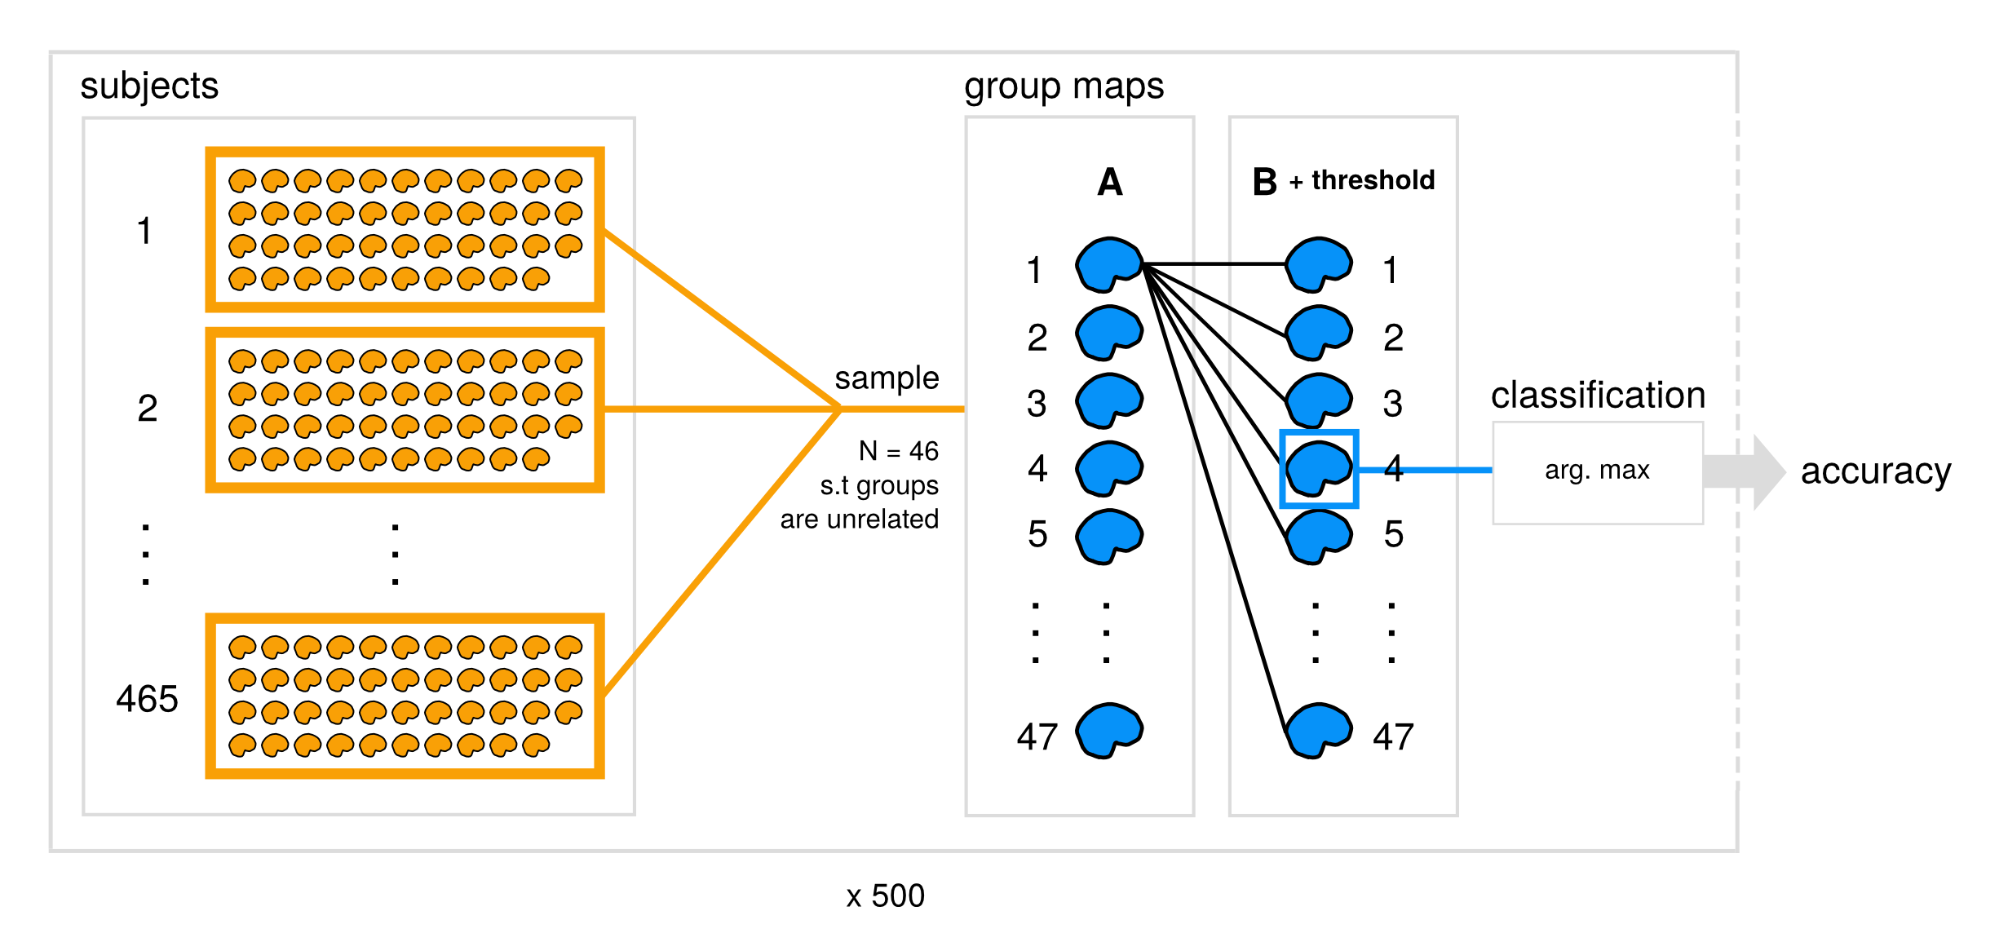
\includegraphics[width=15cm]{images/figure21.png}
\end{center}
 \caption{\label{fig:21} Data generation and analysis process. A subset of 465 datasets from the Human Connectome Project (subjects) is used to generate 47 contrast maps (group maps) for each of groups A and B for 500 subsamples. Within each subsample, an unthresholded image from A is compared with each thresholded image from B with a particular similarity metric and comparison strategy applied.  Each image from A is then assigned the predicted class for the max. arg from the set of B, and accuracy is calculated for the subsample.}
\end{figure}

\section{Results}

\subsection{Assessing the Influence of Thresholding}

\subsubsection{Score Distributions}

Overall, both strategies to handle empty voxels (CCA and SVI) exhibit
decreasing Pearson and Spearman similarity scores with increasing
threshold, and this trend is prevalent whether the thresholding includes
both positive and negative values (\href{https://github.com/vsoch/thesis/blob/master/supplementary/chapter2/supp_figure1A.avi}{Supplementary Video 2.1}), or just
positive values (\href{https://github.com/vsoch/thesis/blob/master/supplementary/chapter2/supp_figure1B.avi}{Supplementary Video 2.2}). For more highly correlated
images, CCA seemed to inflate correlation scores. I observe that a group
of more highly positive correlations present for CCA using positive and
negative values is not present for CCA that includes only positive
values. This suggests that using only positive values to calculate
correlation serves to deflate scores (consistent with the fact that it
is restricting the range of values), and using both positive and
negative values inflates overall scores. It is not clear if this would
be important for distinguishing contrasts of different types in the task
of image comparison. It could be the case that ``deactivations,'' if
they are non-task related will make two images more similar to one
another, but in being consistent across tasks, will act as noise and
decrease accuracy to distinguish different tasks and contrasts from one
another. This finding has been suggested in recent work (see Figure 4)
of Gorgolewski et al. (2015). When comparing CCA with SVI, the group of
more highly positive values is relatively smaller, possibly due to the
fact that the CCA reduces the size of the mask drastically, and the
other strategies do not, for both positive and negative and
only positive values (Figure~\ref{fig:22}).

\begin{figure}[ht!]
\begin{center}
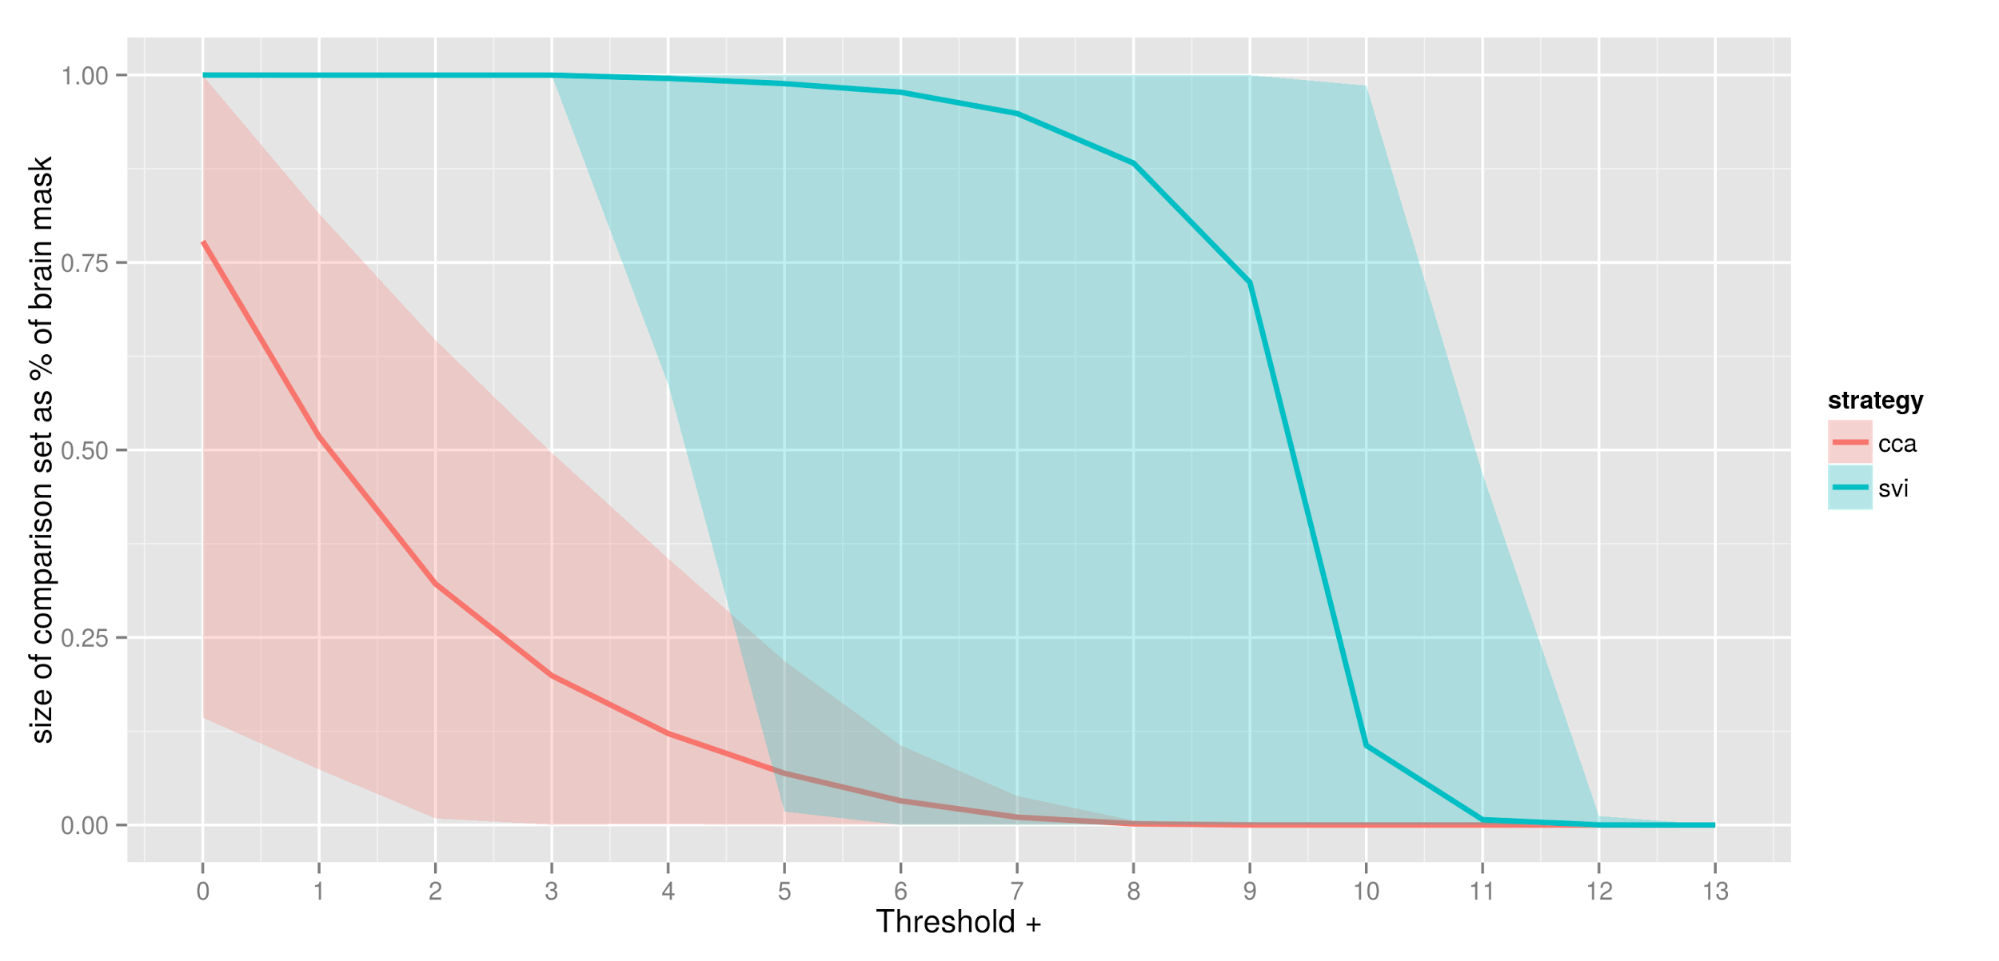
\includegraphics[width=15cm]{images/figure22.png}
\end{center}
\caption{\label{fig:22} The size of the mask across different thresholds for complete case analysis (cca) and single value imputation (svi).}
\end{figure}


\begin{figure}[ht!]
\begin{center}
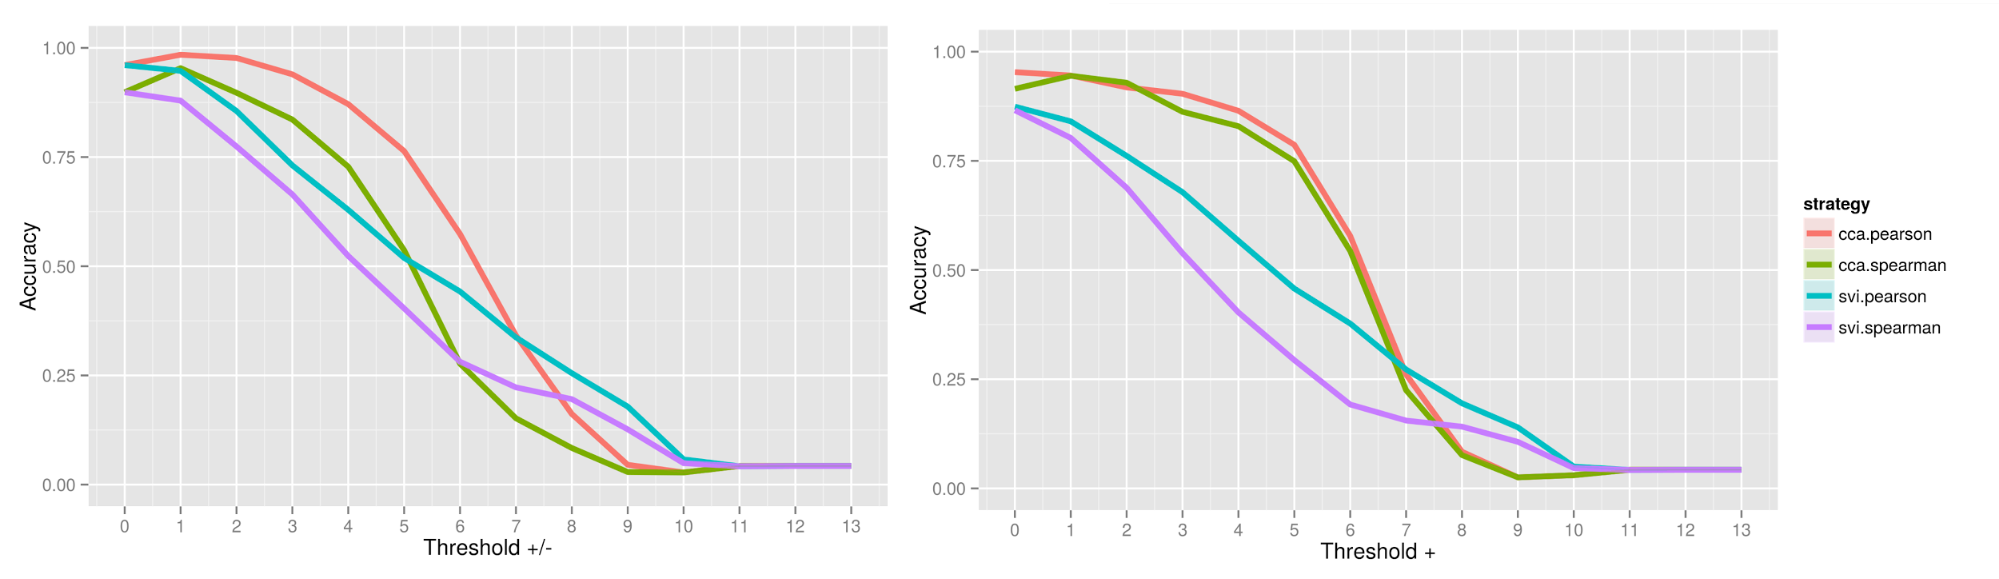
\includegraphics[width=15cm]{images/figure23.png}
\end{center}
 \caption{\label{fig:23} Accuracy of image contrast classification at varying levels of image thresholding, for comparison of an unthresholded image against a set of images at each threshold, including positive and negative values (left) and positive values only (right). Complete case analysis (CCA) with a Pearson score had a maximum accuracy of 0.984 for a threshold of Z = +/- 1.0 (0.983, 0.985), outperforming single-value imputation (SVI).}
\end{figure}

\subsubsection{Thresholding Effects on Classification Accuracy}

When assessing the accuracy of image contrast classification at varying
levels of image thresholding, CCA with Pearson has achieved the highest
accuracy, followed by CCA with Spearman for both positive and negative
values, and only positive values (Figure~\ref{fig:23}).

Accuracy peaks at 0.984 for a threshold of Z = +/-1.0 (95\% confidence
interval, 0.983, 0.985) and at 0.953 for a threshold of Z = 0.0 (no
threshold) (0.951, 0.954), a subtle indication that inclusion of
positive and negative values improves accuracy of rankings globally.
Interestingly, for image comparisons using positive and negative values,
the maximum accuracy does not occur when comparing unthresholded to
unthresholded images, suggesting that values close to 0 may serve as
noise across all images and impede the classification task. When using a
Pearson score for either directionality, a threshold value of Z = +/-3.0
can be used to ensure minimally 0.90 accuracy in returning images of the
same contrast, a threshold that corresponds with images having
approximately only 25\% of overlapping voxels within a standard brain
mask (Figure~\ref{fig:22}A). Investigation of the worst-performing contrast across
folds (working memory task, contrast ``0-back body,'' accuracy = 0.758,
standard deviation = 0.429) showed equivalent highest performance using
CCA with a Pearson score at a threshold of Z = +/-1.0 (Figure~\ref{fig:24}), still
much higher than chance (2\%). Surprisingly, the global peak accuracy of
0.902 (95\% confidence interval, 0.876, 0.928) occurred for a Spearman
score with CCA using positive values only. Complete accuracy results for
combined images across folds are included in \href{https://github.com/vsoch/thesis/blob/master/supplementary/chapter2/supp_data2_ml_accuracy.csv}{Supplementary Data 2.2}, and
for the worst performing image in \href{https://github.com/vsoch/thesis/blob/master/supplementary/chapter2/supp_data3_ml_accuracy_TASK07_CON35.csv}{Supplementary Data 2.3}.

\begin{figure}[ht!]
\begin{center}
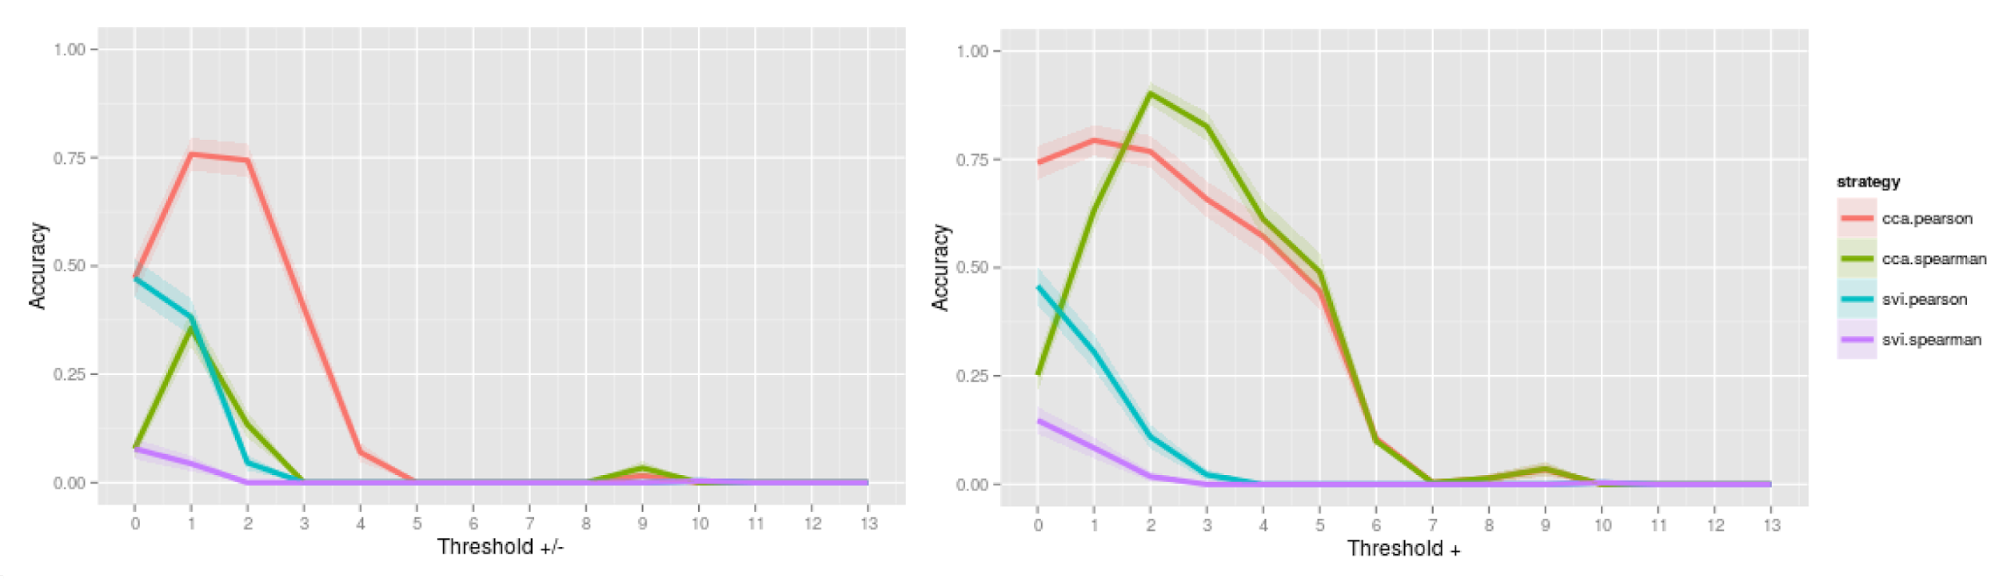
\includegraphics[width=15cm]{images/figure24.png}
\end{center}
 \caption{\label{fig:24} Accuracy of image contrast classification at varying levels of thresholding, for the worst performing image, "0-back body," from the working memory task. Accuracy peaked at a threshold of Z = +/- 1.0 for complete case analysis with a Pearson score and at a threshold of Z = + 2.0 for complete case analysis with a Spearman score for each of positive and negative values (left) and positive values only (right).}
\end{figure}

\subsection{Image Classification}

Across a range of thresholds, very high classification accuracy was
achieved between contrasts, consistent with but substantially better
than previous between-subject classification studies (e.g., Poldrack et
al., 2009). Figure~\ref{fig:25} presents the mean accuracy and standard deviation
for each contrast across 500 random folds for the optimally performing
threshold (Z = +/- 1.0), direction (positive and negative), comparison
strategy (CCA) and similarity metric (Pearson score). Classification is
consistently accurate to distinguish contrasts between tasks (with 30
contrasts being perfectly classified across all 500 folds), and
classification errors are seen for similar contrasts within the same
task (e.g., working memory contrasts ``0-back body'' vs. ``body,''
(overlapping conditions) and gambling task contrasts ``punish,'' vs.
``reward.'') The only misclassification between tasks occurs for the
gambling ``punish - reward'' contrast predicted to be the working memory
``face - average'' contrast. Interactive confusion matrices to explore
the complete result are available
(\href{http://vsoch.github.io/image-comparison-thresholding}{http://vsoch.github.io/image-comparison-thresholding}).

\begin{figure}[ht!]
\begin{center}
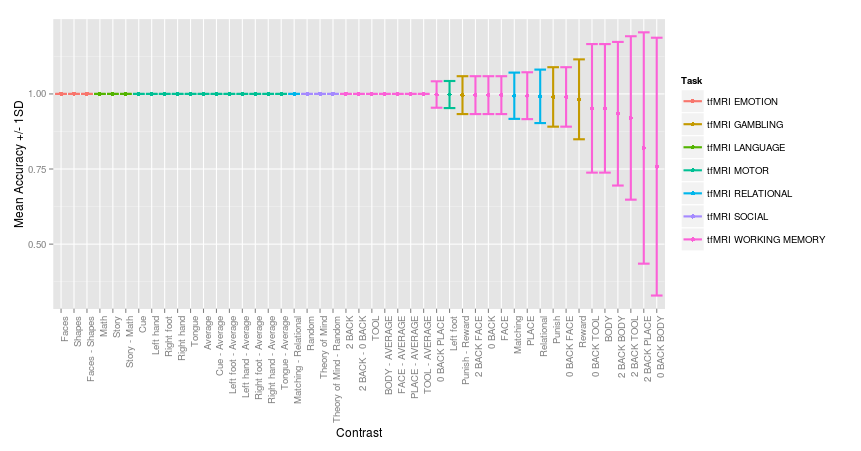
\includegraphics[width=10cm]{images/figure25.png}
\end{center}
\caption{ \label{fig:25} Mean accuracy +/- 1.0 standard deviation for each contrast across 500 random folds for the optimally performing threshold (Z = +/- 1.0), direction (positive and negative), comparison strategy (complete case analysis) and similarity metric (Pearson score). Interactive confusion matrices for all thresholds, comparison strategies, and similarity metrics are available (\href{http://vsoch.github.io/image-comparison-thresholding}{http://vsoch.github.io/image-comparison-thresholding})
\newline \newline}
\end{figure} 

\section{Discussion}

This work quantitatively assesses the impact of thresholding on
performing pairwise image comparison with the two similarity metrics,
Pearson and Spearman rank correlation coefficients. The results suggest
that a small amount of thresholding can improve image similarity
computations. The Pearson metric using maps with both positive and
negative values can be used to optimize classification of contrast maps,
and including maps in the search set that have been thresholded up to Z
= +/-3.0 (corresponding to 25\% of voxels non-empty within a standard
brain mask overlapping between two images) ensures minimally 0.90
accuracy for retrieval of a map of the same contrast. The results
suggest that a minimum degree of thresholding (Z = +/-1.0) can maximize
accuracy of contrasts in a classification framework, and even moderate
thresholding (Z = +/-2.0) can increase accuracy as compared to comparison
of unthresholded maps.

In assessing the distributions of Pearson and Spearman scores, including
both positive and negative values inflate comparison scores for the
higher correlations, however the overall distributions have generally
deflated scores with increasing threshold. This finding is a strength
for the applied task of image comparison given the case that the highest
subset of scores represent ``truly similar'' images. The image comparisons with lower correlations are likely driven by noise at small
values, and so removing these values would deflate the overall score. The slight decrease in accuracy using a Spearman score is likely attributable to the representation of the data in ranked order, suggesting that the values without this transformation carry meaningful signal. However, studying these patterns in the distributions did not serve to answer the question of how classification accuracy is impacted by such thresholding, a question that is answered by an image classification task. In showing that inclusion of positive and negative values serves
to improve accuracy of contrast classification, I suggest that negative
and positive activations are both valuable sources of information,
regardless of the subtle details about if scores are relatively inflated
or deflated across our distributions. This improvement in accuracy could
simply be due to the fact that a comparison is done with twice as many
voxels, however this hypothesis does not hold true when comparing CCA to
single value imputation. CCA, by way of being an intersection, included
substantially fewer voxels than single value imputation, and was
consistently more accurate (Figure~\ref{fig:23}). Overall, these results support a decision to not arbitrarily exclude negative values when performing the
task of image comparison. More work is needed to study the consistency,
or variability, of these deactivations that have been sitting quietly in
statistical brain maps before any consideration of eliminating them is
to be done.

In a classification context, the scores themselves are almost irrelevant
given that the images of the same contrast are returned, however this
statement brings up a very basic question, ``What is the quantitative
language that we should use to compare two images?'' The idea of
~``similar'' is defined on a domain outside of the quantitative, namely,
deriving maps from subjects performing the same behavioral tasks, solely
because there is currently no answer to this question. These analyses
suggest that images thresholded up to Z = +/-3.0 can be used to retrieve a
corresponding contrast 9/10 times, and further, that images can be
thresholded at Z = +/-1.0 to maximize contrast classification performance.

Investigation of the worst performing contrast across folds reveals an
interesting finding that using a Spearman score while including positive
values only can increase classification accuracy by \textasciitilde{} 10\% (for this single image). This particular image, ``0-back body''
from a working memory task, is most commonly misclassified as either
``0-back'' or ``body'' from the same task, an error that is likely
attributable to the subtle differences between these contrasts. In
retrospect, these contrasts are redundant. The contrast ``0-back body''
is a control condition for a working memory task that requires
participants to respond if a body stimulus is presented \cite{Brown2005-sb},
and so the contrast ``0-back'' is the generalization of this task over
different stimulus types, and the contrast ``body'' combines all body
conditions (``0-back'' and ``2-back''). Although these overlapping
contrasts might have been eliminated from the classification task, they
can be used as a case study for comparing two images with subtle
differences. In this scenario, a strategy that would optimize
classification of subtle differences might be used in combination with a
strategy to optimize global accuracy (across tasks). Further, a finding
like this questions the distinctness of these contrasts, and utility in
deriving both. Finally, the inclusion of negative values hindering
ability to distinguish between these similar contrasts again questions
the validity of these ``deactivations'' in the context of highly similar
contrasts. An investigation of the value-added when including negative
values for these highly similar contrasts is warranted.

Importantly, the results question two common opinions on thresholding in
the neuroscience community. First, there is the idea that completely
unthresholded maps are generally superior to thresholded images by way
of providing more data. The results suggest that voxels with very small
values (for our dataset between Z = 0.0 and Z = +/-1.0) primarily serve as
noise, and analyses of unthresholded data may be negatively impacted by
this noise.

Second, the results suggest that standard thresholding strategies,
namely random field theory (RFT) thresholding, may not be optimal for
subsequent image comparison because this strategy eliminates
subthreshold voxels with valuable signal. RFT requires a clusterforming
threshold where only suprathreshold voxels are considered for further
statistical analyses. For example, the popular neuroimaging software
package FSL \cite{Jenkinson2012-pr} has
a standard setting for a clusterforming threshold of Z = +/-2.3 (p
\textless{} 0.01), and the software SPM (Worsley, 2007) uses an even
higher threshold of Z = +/-3.1 (p \textless{} 0.001). To place this
thresholding strategy in the context of this work, I generated
thresholded maps using the FSL standard (Z = +/-2.3) for a single
subsample, including 47 contrasts for each of groups A and B, and
compared the number of voxels within a standard brain mask for these
maps compared to the optimal threshold for this data, Z = +/-1.0
(\href{https://github.com/vsoch/thesis/blob/master/supplementary/chapter2/supp_data4_voxel_counts_rft_vs_thresh.csv}{Supplementary Data 2.4}). I found that a threshold of Z = +/-2.3 produces
maps with on average 28.38\% brain coverage (standard deviation =
16.1\%), corresponding to an average decrease of 38.84\% (standard
deviation = 11.36\%) in the number of brain masked voxels as compared to
the maximum accuracy threshold of Z = +/-1.0. This results in more sparse
results, meaning producing maps with fewer voxels. Mapping this result
into our accuracy space, a threshold of Z = +/-2.3 corresponds with
96.56\% classification accuracy, or a loss of \textasciitilde{}1.86\%
accuracy for image classification as compared to the optimal. This
percentage could be meaningful given a large database of images. A
higher threshold (such as SPM's standard of Z = +/-3.1) would result in a
bigger loss of information and accuracy for image classification.

I have identified an optimal image comparison strategy in the context of
the commonly practiced transformation of image thresholding. I did not
test other transformations, and so I cannot confidently say that using
this transformation of an image is the ``best'' strategy. While
answering this question is outside of the scope of this work, it is a
question that is important to address in order to have consistent
standards for reproducibility, and a common language for both humans and
machines to understand image comparison. This strategy must be developed
by first asking researchers what information is important for them to
understand about the images (e.g., regional or spatial similarity,
temporal similarity), what kind of noise is reasonable to expect given
maps derived in subtly different ways, and then developing a set of
standards to capture and balance those features. Finally, this work does
not claim that there exists a global optimal threshold for such
classification, but rather that researchers should take heed to identify
optimal strategies for thresholding their datasets for use in a
classification framework. The particular threshold values reported in
this study likely depend on the quality of the data, the contrast to
noise ratio, as well as the number of subjects, and thus are not
directly applicable to new datasets.

\subsection{Limitations}
While the initial question behind this work was asking about filtering
an image database based on thresholding (i.e., ``What are the thresholds
that can be included to ensure optimal classification of results?''),
another interpretation of this analysis is about image transformations
(i.e., ``How far can we reduce an image and still get equivalent
results?''). A limitation of this current work is that a more
substantial set of image transformations were not tested. I also start
with the basic assumption that, given that most images are
unthresholded, and sharing of unthresholded images is the direction that
the neuroimaging community is moving toward, a researcher would approach
this task using an unthresholded map as a query image. Fair evaluation
of classification accuracy to compare two thresholded maps would require
a different approach that considers overlap between suprathreshold
voxels in the case of small or non-existent overlap. Without carefully
developed procedure to account for the sparse overlap, I would expect
the classification accuracy to reduce dramatically. Due to this fact it
is recommended to use fully unthresholded maps for sharing purposes (for
example when uploading to repositories such as NeuroVault.org).

The image retrieval task using a statistical map constrained to an
a-priori region of interest is a question not addressed by this work.
The field of image based retrieval is fairly unexplored in context of
statistical maps and some transformation of unthresholded maps might
improve the classification performance. It could be that a
transformation that weights voxels in an intelligent way, a binary
metric, a region-based representation, or another dimensionality
reduction algorithm would be optimal toward this goal. The use of an
intersection mask between an unthresholded image A and thresholded image B also makes our metric asymmetric, and a symmetric metric to compare
such maps might be desired.

The HCP data represents, at the time of this work, the largest publicly
available dataset of single subject task data that allows for this
analyses, and thus inferences are based on this set of images. These
data are of higher quality than many other existing datasets, and it
would be useful to compare the results to other datasets with many tasks
across many subjects. A limitation of using this data is the fact that the acquisition parameters do not vary. However, given that we are operating with group maps derived from many single subjects, and after methods for noise reduction have been applied, arguably additional noise from slight variance in the parameters would not have significant impact on the results, however this would need to be properly tested. These images shared acquisition parameters, voxel
dimensions, and smoothing, and while it is relatively easy to transform
images into a common space and size, deviance in our findings can not
be predicted for different datasets. Finally, these analyses are focused
on group statistical maps. Retrieval of contrast images for
single-subject maps would be much more challenging due to the
possibility of large inter-subject variability.

\section{Conclusion}

I have investigated the impact of thresholding on contrast
classification, and suggested specific strategies to take when
performing image comparison with unthresholded maps. This work is
important, because voxel-wise image comparison I believe will drive the next decade of meta-analysis. The applicability
of my work is immediate as I have used these findings to drive the first
version of our ``image comparison'' feature newly released in
http://www.neurovault.org. While there are many questions to be
investigated pertaining to the simple task of image comparison and the
more complicated task of doing meta-analysis, this work is a first step
toward deriving a holistic understanding of how to ``best'' compare the
expanding landscape of publicly available statistical brain maps.

\chapter{Semantic Image Comparison}
Here I present automated and openly available infrastructure and methods that I have developed for semantic classification of
statistical brain maps, and demonstrate that such a comparison is
comparable to the more commonly done calculation of spatial similarity (Specific Aim \#2: to assess semantic image comparison against traditional
  approaches). This chapter presents rationale for integrating semantic information into the task of image comparison for meta-analysis of statistical brain maps, specifically in a classification
framework. Demonstrating that semantic annotations carry equally valuable signal to spatial comparisons would reduce computationally complexity in the comparison, bring rich ontological standards to the description of statistical brain maps, and allow for better interpretation of the maps themselves.

\section{Semantic Comparison of Statistical Brain Maps}
Statistical brain maps carry a wealth of information to inform our
understanding of the human brain. Underlying the matrix of numbers that
is the most commonly utilized output of a neuroimaging analysis is a
resource that has yet to be shown to be useful: semantic knowledge. Computational approaches to performing common investigations such as meta-analysis and assessment of reproducibility are the standard because
proper semantic annotation of this data is incredibly challenging if not
totally unfeasible for large data. Given this challenge, it is not
clear if semantic information about statistical brain maps can be useful
in a classification framework. ~This semantic understanding~will improve
the typical workflow of the neuroimaging scientist by allowing them to
immediately place any~statistical brain map in the context of results
that came before it, providing an intuitive transition from data and
knowledge.

Several barriers related to infrastructure and manpower have, to this
day, existed to further complicate this goal. First, results in the form
of statistical brain maps have not been shared. This is changing with
public databases and openly available datasets \cite{Gorgolewski2015-gu,Van_Essen2013-fi,Hall2012-qo,Reid2015-gt}, and so now it is very feasible to quickly share an entire statistical
map or full raw dataset. Further, integrated into some of these
resources are application programming interfaces (APIs) that serve to
connect these data to other resources, allowing for automated,
integrated analysis. Of particular interest, and previously described is the Cognitive Atlas \cite{Poldrack2011-jp}, an open-source knowledge-base that represents an understanding of
cognitive processes, experimental paradigms, and the relationships
between them. This ontology has existed for over 11 years, and with
substantial contribution from experts in the field, now has embedded
detailed relationships that are comprehensive enough to be useful for
making inferences. It is now possible to upload data to a database such
as NeuroVault, tag the data with the specific measurement that is
represented by some comparison~over experimental conditions (called a
``contrast''), and programatically be able to make an association
between the brain map and the cognitive concepts that it represents.

In this work, I present the first ontologically-driven, automated
semantic image comparison to demonstrate that there is value in these
semantic annotations. My approach is two-fold. I first assess semantic
comparison in a classification framework, using a multi-label machine
learning encoding model to predict brain images from cognitive concepts.
I then use a graph metric commonly utilized to assess the similarity of
gene sets to compare brain statistical maps based on cognitive concepts
they are tagged with. I demonstrate with representational similarity
analysis that semantic image comparison is comparable to the more
commonly done calculation of spatial image comparison, the current
standard. This work presents strong evidence for the further development
and use of such methods to assist in the larger goal of image-based
meta-analysis.

\section{Methods}

\subsection{Overview of Open Infrastructure}

This work uses completely openly available data (accessible via API) and
methods (publicly released packages) for performing all analyses and
visualization. I first select a set of publicly available brain maps
from the NeuroVault database, and annotate
these maps with terms defined in the Cognitive Atlas to generate a
concept graph describing concepts, tasks, and their relationships. By way of recently released
infrastructure to tag images with contrasts from the Cognitive Atlas in
NeuroVault, images are immediately mapped to this tree under the
concepts they represent, allowing for a completely semantic-based image
comparison analysis. I test the predictive ability of semantic
annotations in a classification framework (Section 3.2.3 Semantic image
comparison in a classification framework), and show value in semantic
image comparison by comparing to the current standard, spatial
similarity (Section 3.2.5 Comparison of semantic to spatial similarity),
and then. An overview of the approach is provided in Figure~\ref{fig:31}, scripts
with robust documentation to reproduce all analysis are available \cite{Vsoch_undated-mq}.

\begin{figure}[ht!]
\begin{center}
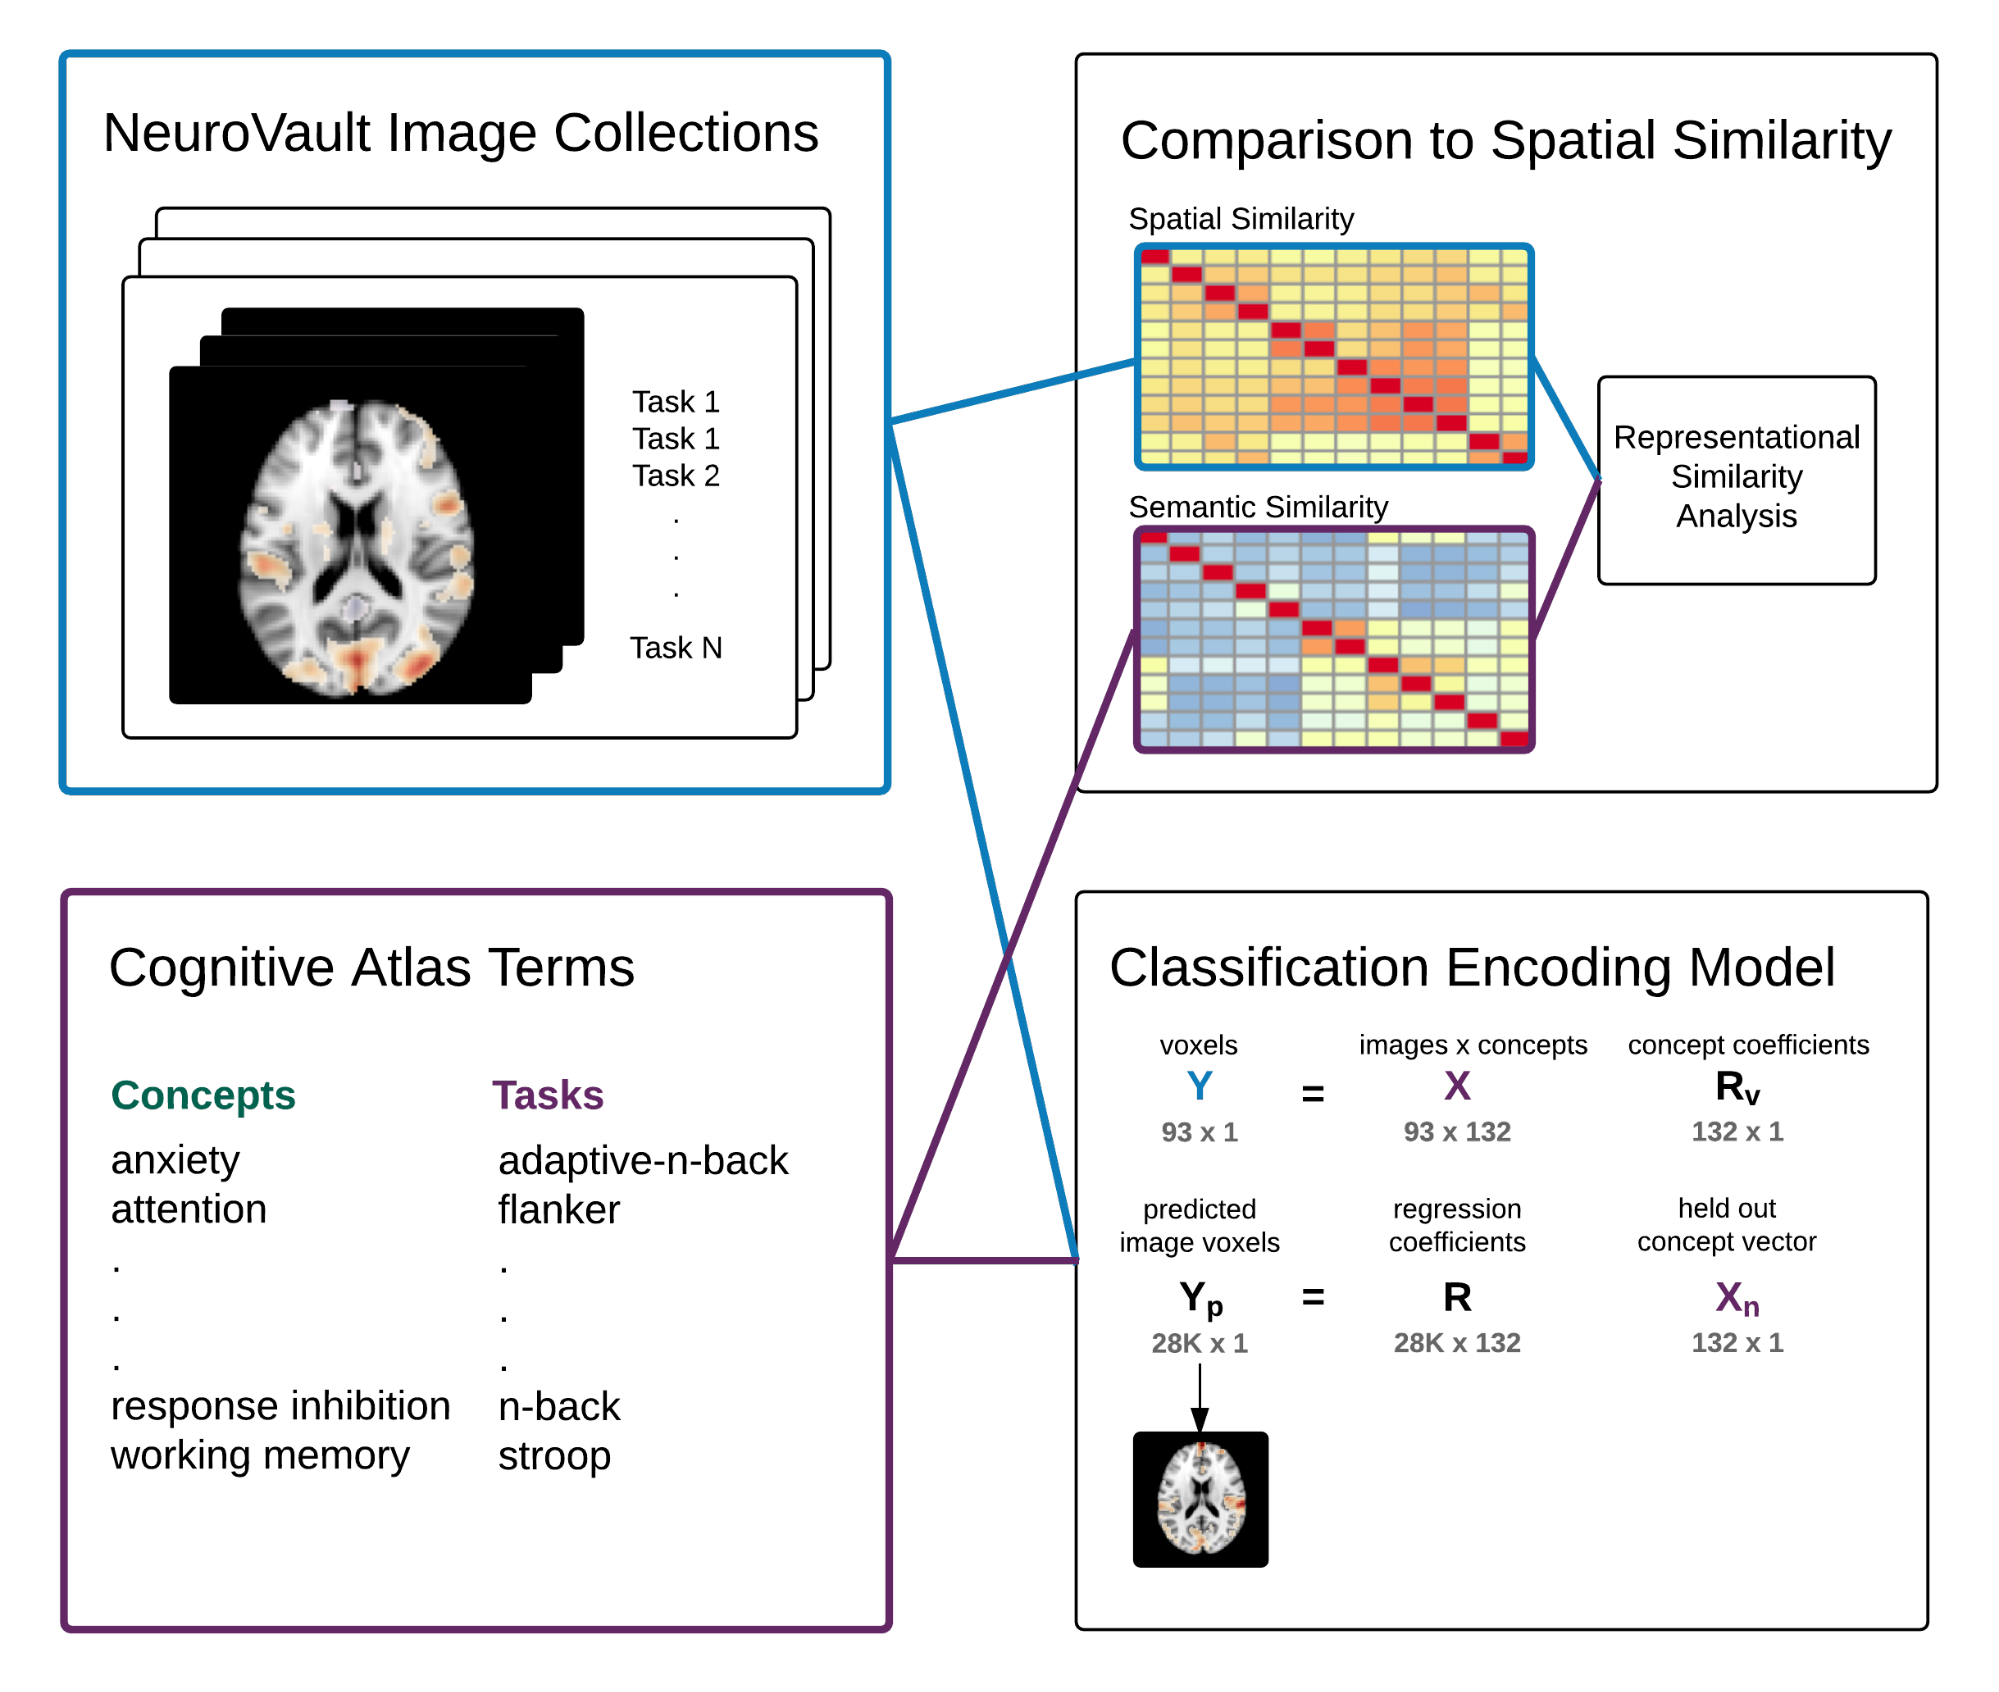
\includegraphics[width=10cm]{images/figure31.png}
\end{center}
\caption{ \label{fig:31} Overview of the approach. Group statistical brain maps
annotated with Cognitive Atlas concepts come from the NeuroVault
database (top left), and concept relationships are represented in the
Cognitive Atlas (bottom right). Spatial similarity is compared to purely
semantic similarity using representational similarity analysis (top
right), and a classification encoding model is used to test the
predictive ability of semantic annotations (bottom right). An encoding
model is generated at each voxel to predict a vector of 93 image voxels
(Y) using concept labels (X) excluding two held out images, generating a
vector of 132 coefficients (R) for each of v voxels. These vectors can
be assembled into a matrix (R) to generate a predicted image (Yp) using
a held out concept vector (Xn).
\newline \newline}
\end{figure} 


\subsection{Data and Curation}

\subsubsection{NeuroVault}

The NeuroVault database is a valuable resource for the sharing of
statistical brain maps, each the result of an experiment to measure a
cognitive process, as well as tools to annotate these maps. Researchers
are incentivized to upload their maps here either for purpose of data
sharing (such as for a journal requirement), visualization of maps, or
as an easy way to archive a result for long term reproducibility. To
prepare NeuroVault for this application, I first added the ability of
NeuroVault users to tag brain maps with contrast labels from tasks
defined in the Cognitive Atlas
 \cite{NeuroVault_undated-gr}.
To select datasets, I filtered images to include those with a DOI, in
MNI space, and which were~unthresholded. This resulted in 93 statistical
brain maps across 22 collections, including both Z and T maps. I use a
method described previously \cite{Sochat2015-qs} to
convert T score maps to Z score maps, obtaining the number of subjects,
N, in each study to calculate the degrees of freedom (N-2) using the
NeuroVault API. All maps are resampled to a MNI 2mm standard brain.

\subsubsection{Cognitive Atlas}

The Cognitive Atlas is a community effort to define tasks and associated
concepts studied in cognitive neuroscience, and the relationships
between them. As an ontology, it maps nicely onto a graph framework in
that entities (concepts and tasks) are represented by nodes in a graph,
and the relationships between them are the connections. By describing
tasks in the language of concepts that encompass these nodes, and
mapping brain image results to this tree, I can walk along the branches
to understand how something like ``theory of mind'' relates to
``anxiety,'' and perform computations on the graph to describe the
universe of brain imaging results in this context. Toward this goal,
we~first annotated contrasts from experimental paradigm with the
concepts they measure,~and then defined relationships between them,
discussed next.

\paragraph{Concept association with contrasts}

it is only possible to~make inferences about how a concept like
``anxiety'' is represented by a particular statistical brain map result
given an understanding about the cognitive concepts that are queried by
a large set of experiments. This information, the relationship between a
task's contrast (e.g., ``angry faces minus baseline'') and the measured
concepts (e.g., ``anxiety''), is called an ``assertion'' and these
assertions make up the relationships of the Cognitive Atlas.

Toward this goal, the Poldrack Lab at Stanford University established a
regularly meeting Cognitive Atlas Annotation group that would review a
set of contrast images publicly available in NeuroVault, and generate a list of cognitive concepts queried by each
one. This process included communication with experts in the field, and
care was taken to contact the owners of each dataset described in the
NeuroVault database to discuss the task and confirm tagged cognitive
contrasts. I have made our process available, including ``best
practices'' for other researchers to do the same \cite{Vsoch_undated-gw}.
This procedure provided a list of 132 concepts defined in the Cognitive
Atlas across 29 cognitive paradigms that were represented by the 93
maps.

\paragraph{Definition of relationships in Cognitive Atlas}

One of the strengths of an ontology like the Cognitive Atlas comes by
way of making assertions that entities, in this case the cognitive
concepts, are meaningfully related. ~These relationships are the links
in the graph, defined by the OBO Relations Ontology \cite{Mungall2015-yh},
of which the Cognitive Atlas uses ``is a'' and ``part of.'' For example,
the ``part of'' relationship formally states, ``Everything is part of
itself. Any part of any part of a thing is itself part of that thing.
Two distinct things cannot be part of each other.'' Applied to concepts
in the Cognitive Atlas, an example would be ``emotion regulation'' is a
part of ``emotional expression,'' and this assertion was made because
regulation of emotion is an essential component for the expression of an
emotion. I represent these relationships as different weights attributed
to links in the graph. I made an effort to contact 35 ``experts'' in
cognitive psychology to elicit contribution to the atlas, however
participation was not substantial enough to propose as the sole method
for defining such relationships. I selected a subset of the ontology
under the category of ``Reasoning and Decision Making'' for which the
Poldrack Lab has expertise
\cite{Bissett2012-aq,Bissett2014-td,Bissett2011-of,Bissett2012-yu,Bissett2013-ep,Yamaguchi2012-yn,Poldrack2009-ux,Poldrack2011-jp,Lenartowicz2010-bh,Tom2007-kx,Poldrack1999-cr},
and spent many months going through each concept to review both the
assertions (concept ``is a kind of'' and ``is a part of'') to ensure
that the tree was not sparse. I believe that the group expertise,
combined with expert opinion of collaborators, produces a graph that is
suitable to describe relationships between these 93 maps.

\subsection{Semantic image comparison in a classification framework}
To test the predictive value of semantic annotations, I employ an
encoding model that generated a predicted brain image based on a binary
vector of concept labels, and used a leave-two out classification method
to assess accuracy. To generate an encoding model, I train a regularized
linear classifier, the elastic net
 \cite{noauthor_undated-wy} at
each voxel to generate sparse regression coefficients for each concept
that can be multiplied by a new concept vector to generate the predicted
image. This approach will be applied to two datasets to demonstrate its validity: first in the context of whole brain statistical maps (IBMA) using the 93 result contrast images from the NeuroVault database, and second in the context of coordinate-based statistical maps (CBMA) using the NeuroSynth database (\cite{Yarkoni2011-rg}).

\subsubsection{Prediction of whole brain statistical maps using cognitive concepts}
This analysis aims to demonstrate the utility of semantic annotations of whole brain statistical maps to predict whole brain statistical maps. Specifically, we want to show that a vector of binary concept labels for a held out image can be used to generate a predicted image with a pattern of spatial activation consistent with the actual image. I define the training data, X as a 93 by 132 matrix of images by
concepts, where each value is a binary indicator if the image is tagged
with the concept. I define the Y as a vector of 93 voxel values, one for
each image, and by building a model at each voxel to output a vector of
132 coefficients, I can assemble this into a regression parameter matrix
R of size 28,549 (voxels) by 132 (concepts). The assessment of 28,549
voxels is due to the need to resample the original 2mm brain maps to 4mm
in order to make the analysis computationally tractable. I can then
multiple a new image, N, represented by a binary concept vector of 132
by 1 to generate a predicted image of size 28,549 by 1.~An illustration
of this procedure is provided in the bottom right panel of Figure~\ref{fig:31}.

Using the encoding procedure detailed above, for each set of pairwise
images in the set, I performed the following procedure to generate
predictions for two held-out images: \newline

\textbf{for image1 in all images:} \newline
\indent \indent \textbf{for image2 in all images} \newline
\indent \indent \indent if image1 != image2 and contrast of image1 != contrast of
image2:\newline
\indent \indent \indent \indent hold out image1 and image2, build encoding model using other \newline
\indent \indent \indent \indent generated predicted image PR1 for image1   \newline  
\indent \indent \indent \indent generated predicted image PR2 for image2   \newline  
\indent \indent \indent \indent classify image1 as being more similar to PR1 or PR2 using
spatial similarity \newline
\indent \indent \indent \indent classify image2 as being more similar to PR1 or PR2 using spatial similarity \newline
\indent \indent \indent \indent assign correct classification if image1 is more similar to
PR1 \newline
\indent \indent \indent \indent assign correct classification if image2 is more similar to
PR2 \newline

Essentially, we are building a model using all but two held-out images (image1 and image2), and then predicting the statistical brain maps for those images (PR1 and PR2) based on the terms the images are annotated with. This produces two classifications per hold-out, and for each, we call the classification correct if the predicted image (for example, PR1) is spatially more similar to its actual (for example, image1) than the actual second image (for this example, image2). I do not include images in the assessment with equivalent contrast
labels, for a final potential comparison set of N=8556. To assess
spatial similarity I use the same complete case analysis procedure
discussed in 2.2.2. Running this procedure for all unique pairwise
images will result in two predictions per set, each of which can be
correct or incorrect, for a total of 17,112 predictions. To calculate an
overall accuracy, I calculate the number correct divided by the total
predictions: \newline

~ ~ ~ accuracy = \underline{number correct}

 ~ ~ ~ ~ ~ ~ ~ ~ ~ ~  ~total predictions

\paragraph{Classifier Validation}

To assess if this accuracy value is significantly different from chance,
I perform the procedure for prediction of whole brain statistical maps as previously explained 1000~times
with~\textasciitilde{}1000 image sets, but randomly
shuffling the image labels to generate a null distribution of 1000
accuracies. I can then calculate a p-value to assess where the actual accuracy falls in this distribution, and assess if the actual
accuracy is significantly different from this null distribution of
accuracies that represent the classification procedure under random
chance. Finally, I~generate a confusion matrix of images by images to
assess which images are commonly mistaken for other images.

\paragraph{Learned Concept Map Validation}

Assessing the frequency for which each cognitive concept is associated
with correct or incorrect classification gives insight to the quality of
the cognitive concepts themselves. Toward this goal, I generated a
concept confusion matrix, where each row is a single concept from the
Cognitive Atlas, and the columns are counts for the number of times the
concept was associated with a correct prediction (``correct''), and the
number of times a concept was associated with an incorrect prediction
(``incorrect''). Given that brain maps in the NeuroVault database are
organized by cognitive paradigm (task) and collection (a group of images
uploaded by a researcher), I would also be interested in knowing the
frequency at which an incorrect prediction (all values of the matrix not
in the diagonal) could be labeled as a within-collection (between-task)
confusion, a between-task confusion, or between-collection
confusion. I can generate these values by assigning each box in the confusion matrix to one of these categories depending on the relationship between the two images, and then summing the confusion values for each category, and
dividing by the total number of confusion values. This procedure will
produce one value per category representing the percentage of incorrect
predictions that are within-collection (between-task), between-task, or
between-collection.

Finally, as each concept is associated with a vector of voxels, one for
each in a brain map, I can reconstruct the vector into a standardized
(Z-scored) brain map to visualize the coefficient learned at each model.
This is a form of soft validation that will allow us to view what the
model has learned about each cognitive concept from a set of annotated
images.

\subsubsection{Prediction of coordinate-based statistical brain maps using cognitive concepts}
The previous analysis is suited to demonstrate the value of semantic annotations in the context of whole brain statistical maps, and this next analysis aims to show that semantic annotations also have predictive value in the context of coordinate-based data. The NeuroSynth database (\cite{Yarkoni2011-rg}) is a well-established, automatically derived database that associated x,y,z coordinate reports in papers with terms from the abstract. At the time of this analysis, the database contained 11,405 abstracts, each associated with a set of coordinates. As previously described, NeuroSynth provides, for each abstract, a normalized value to reflect the prevalence of each term within an abstract, and uses these associations to derive the probability of activation given a term (feature) given a set of input abstracts (Section 1.2.1). As I am interested in a specific set of cognitive concept terms from the Cognitive Atlas, many not represented in the NeuroSynth term set, I obtained the original set of 11,405 abstracts, and re-generated these normalized tables using the same procedure defined in \cite{Yarkoni2011-rg}. Terms were filtered to include only those present in 10 or more abstracts. This procedure produced a table of abstracts by 399 terms, a number that is substantially larger than the 132 from the previous analysis, as we are not limited to the terms annotated via the 93 images. This matrix, Y, of size 11,405 by 399, contains the annotations for each abstract that will be used to predict the coordinate-based brain maps.

To generate the coordinate-based maps, I resample the binary coordinate data (a 1 indicates the coordinate is reported in the paper associated with an abstract) to a 4mm space, and this provides a sparse brain image associated with each abstract. I next use this data in the equivalent context as the 93 NeuroVault images: we want to show that the vector of 399 concept labels can be used to predict the coordinate data. We employ the equivalent classification framework, however instead of holding out two images to make two predictions per iteration, we hold out approximately 1\% of abstracts at each iteration, building the encoding model from the other 99\%. We can then, for all pairwise images in the holdout set, use the trained model to generate the predicted images, and test whether the similarity is higher between the true and predicted for each pair. The calculation of accuracy is equivalent to as before, a ratio between the number of correct predictions out of all predictions.


\subsection{Comparison of semantic to spatial similarity}

An assessment of semantic comparison of brain maps, independent of any
operations on the spatially defined values, would be valuable to compare
against the standard of using a voxelwise metric. Toward this goal, I
first wanted to develop a graph-based metric for semantic image
comparison that would derive similarity from semantic annotations and
relationships represented as weights in the graph. The cognitive concepts are vertices in the graph, and each contrast image then is a set of vertices. First I will review graph metrics to compare vertices, and then discuss application of these metrics to compare sets of vertices.

\subsubsection{Semantic Comparison of Graphs}
The majority of similarity metrics for graphs are based on comparing vertices. For the task of comparison of semantic terms, we could arguably use any of these method derivations, and would want to choose the one that produces a similarity matrix that is most similar to spatial image comparison. Specifically, well-known methods include:

\begin{itemize}
\item
  \textbf{ASCOS}: "Asymmetric network Structure COntext Similarity" infers the similarity between nodes based solely on structure context, i.e., the patterns of the edges, because nodes with similar structure are likely to have similar attributes. This algorithm is similar to a well-known algorithm called SimRank, however due to comparing all paths between nodes, ASCOS tends to outperform SimRank \cite{6785743}
\item
  \textbf{COSINE}: If the i-th and j-th rows/columns of an adjecency matrix are regarded as two vectors, then we can calculate the cosine of the angle between them to derive a similarity measure. The cosine similarity of i and j is the number of common neighbors divided by the geometric mean of their degrees. \cite{Salton:1989:ATP:77013}
\item
  \textbf{JACCARD}: calculates the number of common neighbors divided by number of vertices that are neighbors of at least one of the two vertices being considered. \cite{jaccard}
\item
  \textbf{KATZ}: Katz centrality computes the relative influence of a node within a network by measuring the number of the immediate neighbors and other nodes that connect to the node via the immediate neighbors. Connections to distant neighbors are penalized by an attenuation factor \cite{Hanneman_undated-ou}
\item
  \textbf{LHN}: "Leicht-Holme-Newman" takes after Jaccard, but "punishes" the high degree nodes even more \cite{Leicht2005-dv}.
\item 
  \textbf{DICE}: is twice the number of common neighbors divided by the sum of the degrees of the vertices \cite{10.2307/1932409}
\item
  \textbf{INVERSE LOG WEIGHTED}: is the number of common neighbors weighted by the inverse logarithm of their degrees. The rationale for this approach is the idea that two vertices should be considered more similar if they share a low-degree common neighbor \cite{Adamic2003-mj}.
\end{itemize}

The Cognitive Atlas concept space consists of cognitive concepts linked by relationship types "is a kind of" and "is a part of," and simple graphs can be generated that represent links with one or both of these edges. To calculate pairwise comparison of cognitive concepts, I \href{https://github.com/vsoch/semantic-image-comparison/blob/master/analysis/graph/similarity.py}{implemented these metrics} and used networkx \cite{hagberg-2008-exploring} to generate a graph to represent each of the "part of," and "kind of" relationships, and the two combined. I could then use these concept similarity matrices to calculate similarity between image contrasts by the following procedure for some square concept similarity matrix, df, and two sets of cognitive concepts, C1 and C2: \newline

\indent Subset rows of df to C1 and sum across rows \newline
\indent \indent Subset columns to C2 and sum across columns \newline
\indent \indent \indent Divide by number of concepts in set(C1,C2) \newline

The above procedure produces a mean similarity score between the two sets of concepts for a contrast of interest. To supplement these metrics, we can also include a well-known method to compare gene sets using the Gene Ontology \cite{Wang2007-nt}. While many methods from this space rely on having annotated databases \cite{Mistry2008} or finding enrichment of genes in some list \cite{Eden2009}, Wang is ideal for this application because it does not need an annotated database of terms or probabilities. I developed an R
package \cite{CognitiveAtlas_undated-hk}
that can take as input a contrast defined in the Cognitive Atlas, and return
such a score. The metric is based on Wang's metric \cite{Wang2007-nt},
which has had most wide application to compare gene sets. The metric
aims to assess the semantic contribution of ancestor terms. This means
that for any two concepts, C1 and C2 in the graph, one can walk up the
tree and define a list of concept nodes, and associated ``is a'' and
``part of'' relationships between these nodes, all the way to the
highest (parent) base node of the ontology. The weight for each concept
is determined by multiplying the last (child node) weight by~0.8 for
``is a'' relationships, and 0.6 for ``part of'' relationships, as
implemented in the initial paper
\cite{Wang2007-nt}, and I believe to be a reasonable weighting to reflect similarity of a
type of synonym (``is a'') or (``part of''). The multiplication means
that weights decrease as one moves up the tree toward the root. I then
take the intersection of concepts between C1 and C2, and the similarity
score is calculated as the ratio of intersected weights~to all the
weights~defined between the two concepts. \newline

similarity = ~ ~ ~ \underline{sum(intersected weights)}

~ ~ ~ ~ ~ ~ ~ ~ ~ ~ ~ ~ ~ ~ sum(all weights)\newline \newline

This procedure derives a single score to compare each pairwise concept
defined in the ontology tree, and forms a matrix that can be used for
comparison to a spatial similarity.

One would have confidence that the graph method is capturing meaningful
relationships between brain maps if the semantic similarity matrices are
comparable to a spatially derived equivalent matrix. Thus, for the final
step of validation I compared spatial and semantic similarity. Maps that
query more similar cognitive processes should have higher spatial
similarity.

\subsubsection{Derivation of spatial similarity matrix}

To assess the spatial similarity of maps, I used an approach from
recently published work \cite{Sochat2015-qs} to derive pairwise comparison of the 93 statistical brain maps maps using
complete case analysis with a pearson score. While this work found an
optimal classification accuracy for image contrasts using a threshold of
Z=+/-1, I chose to use the unthresholded maps, as this is the
transformation that was used for the~semantic similarity
assessment,~maximizes the comparison set between the two images, and is
not significantly different from a threshold of Z=+/-1 \cite{Sochat2015-qs}.
The approach is as follows:

For each of the 93 NeuroVault maps, N1: \newline

~ ~ For each of the 93 NeuroVault maps, N2:

~ ~ ~ ~ generate a pairwise deletion mask (complete case analysis)

~ ~ ~ ~ ~ ~ calculate pearson score\newline

This procedure resulted in a matrix of spatial image comparisons to
compare the semantic comparisons to.

\subsubsection{Representational similarity analysis}

Representation similarity analysis (RSA) is a simple method to compare
the similarity of two matrices based on a pearson correlation
coefficient between corresponding upper triangles \cite{Kriegeskorte2008-kg}.
I used RSA to make an assessment of the semantic image comparison
similarity matrix defined in 3.2.5 against a spatial image comparison
matrix defined in the previous section. This procedure can also be done for
submatrices, for example, filtering the matrix to images that are
relevant to a specific cognitive concept or paradigm. These scores
provide an overall similarity of semantically and spatially derived
image comparisons globally, as well as within task and concept groups.

\section{Results}

\subsection{Semantic image comparison in a classification framework}

\subsubsection{Prediction of whole-brain statistical maps using cognitive concepts}
I used a voxelwise encoding model to test the predictive ability of
semantic annotations in a classification framework for 93 whole brain statistical maps from the NeuroVault database. ~There were a
total of 7209 correct predictions out of a total of 8554 predictions
(accuracy = 0.843), and comparison against the null distribution of
accuracies (N=1000) produced a mean accuracy of 0.49
(p\textless{}0.001), demonstrating that a classification procedure using
semantic information performs well above chance. A full normalized
confusion matrix \href{https://github.com/vsoch/semantic-image-comparison/blob/master/update/encoding_regression_performance/classification_confusion_binary_4mm_perform_norm.tsv}{is available}.

\paragraph{Learned Concept Map Validation}

The top concepts most commonly associated with correct prediction
included, face maintenance, left hand response execution, body
maintenance, place maintenance, and pattern recognition with correct prediction of all
associated images. Concepts most commonly associated with incorrect
prediction included context representation, mental representation, and monetary reward prediction error, correctly
predicting associated images approximately 0.17 of the time. The full
concept confusion matrix with correct frequency, incorrect frequency,
and image counts is available as
\href{https://github.com/vsoch/semantic-image-comparison/blob/master/update/encoding_regression_performance/classification_concept_confusion_norm_perform.tsv}{is available}. Within the incorrect predictions, we would want to know if the
proportion of confusions can be attributed to a particular relationship
type. For example, confusions can occur when two contrast images belong
to the same task (within-task), or when images are from the same
collection but have different tasks (between-task). Finally, images can
be from entirely different collections (between-collection). To
determine these proportions, we counted the number of confusions that
occurred within-collection (between-task), within-task, and
between-collection, and normalized by the total number of images within
each category. The rates of within-task, within-collection
(between-task), and between-collection were 0.24 ( 76/322 ), 0.20 (
93/450 ), and 0.23 ( 1798/7784 ), respectively. While we would have expected more
images to be confused within-task (e.g., memory paradigms often query
the same processes but use different stimuli such as houses, tools, or
faces), this result suggests that the cause of error was perhaps
more consistent between classes. Visual inspection of several of the highly
confused images revealed maps with highly robust spatial activation,
suggesting that the common error might be attributed to lack of distinct
spatial pattern. To visualize the concepts, an example of best and worst
predictive concept-specific Z-score brain maps generated from the
regression parameters are provided in Figure~\ref{fig:32}. All regression parameter
maps are publicly available in the NeuroVault database
(\href{http://neurovault.org/collections/1170/}{http://neurovault.org/collections/1170/}).

\begin{figure}[ht!]
\begin{center}
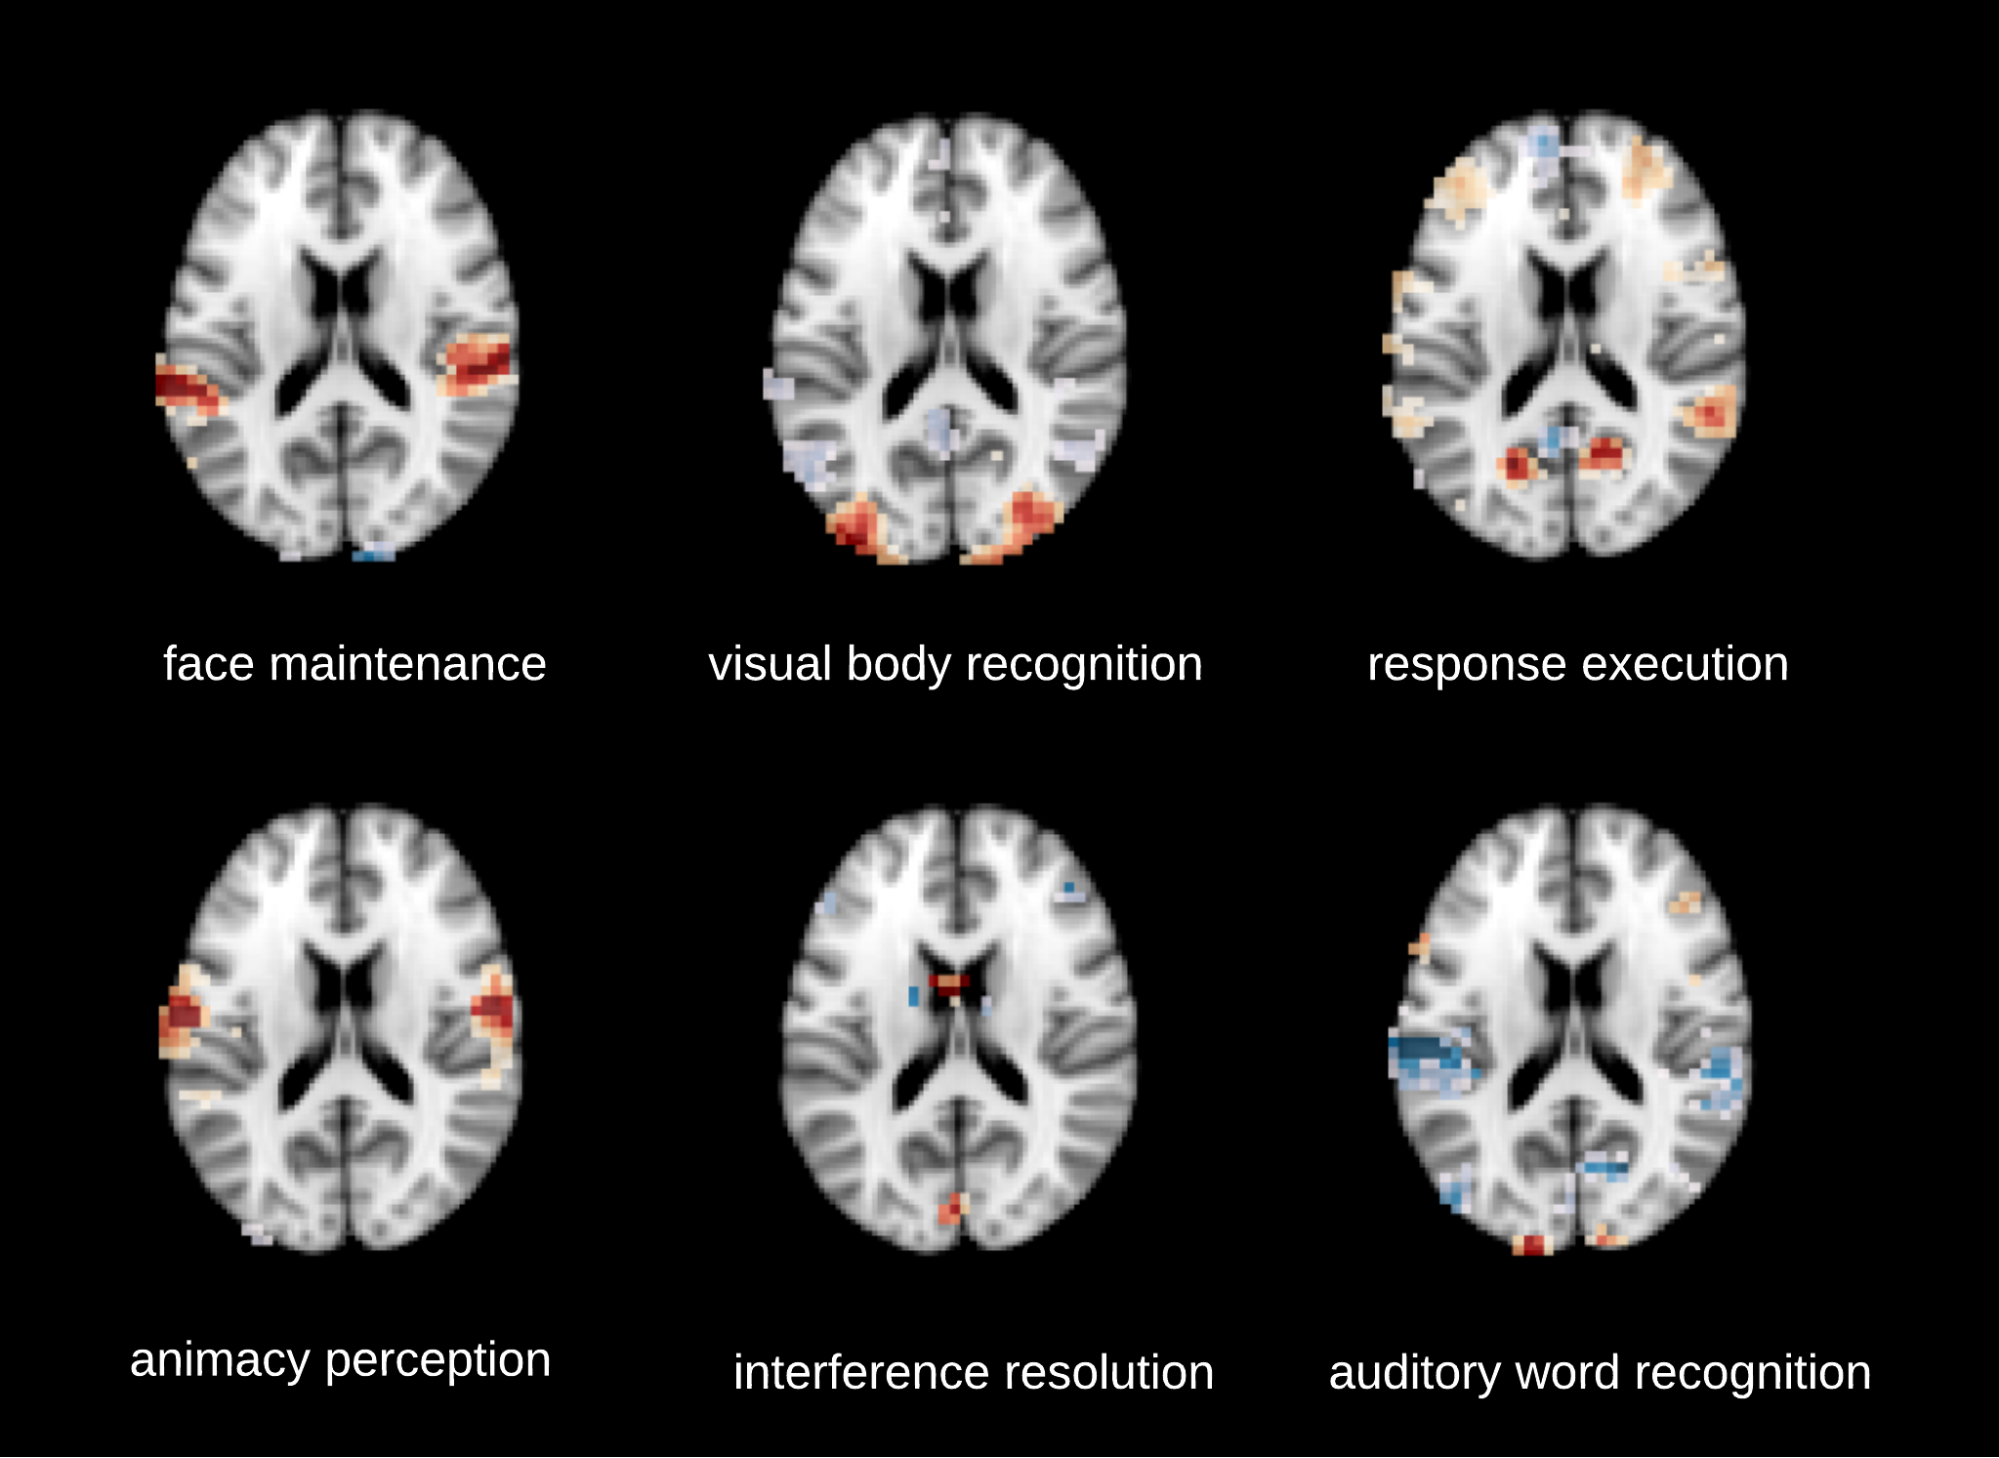
\includegraphics[width=15cm]{images/figure32.png}
\end{center}
 \caption{\label{fig:32} Concepts associated with correct and incorrect predictions.
Regression parameters from the encoding model reconstructed into brain
maps to provide a visual understanding of what the model learned, for
concepts consistently associated with correct predictions (top row), and
associated with incorrect predictions (bottom row). Maps used in the
classification task included voxelwise data, and are thresholded above
to show the highest positive (red) and negative (blue) values.}
\end{figure}

\subsubsection{Prediction of coordinate-based statistical maps using cognitive concepts}
The voxelwise encoding models used to assess the predictive ability of
semantic annotations using coordinate-based image data from the NeuroSynth database in a classification framework were generated for each of 101 iterations, each encompassing approimately 1\% of NeuroSynth abstracts. Across the 101 iterations, there were 644,106 comparisons and 438,600 were correct for an accuracy of 0.68.


\subsection{Comparison of semantic to spatial similarity}

Comparing a spatial similarity matrix to matrices of semantic image comparison scores (derived from the ascos, jacaard, katz, lhn, inverse log weighted, dice, and cosine similarity metrics) using representational similarity analysis (RSA) was used to assess if semantic image comparison is similar to spatial, and further, what level of relationships ("is a kind of", "is a part of" or both combined) produces stronger correlation with spatial similarity. A matrix of semantic image comparisons, done by way of the Wang metric implemented in cogat-similaR \cite{CognitiveAtlas_undated-hk} was also compared. Across all comparisons, the highest RSA scores resulted from katz similarity using "part of" relationships (RSA correlation = 0.536), ascos similarity using both relationships (RSA correlation = 0.526), and then the Wang metric (RSA correlation = 0.514). The direct comparison between spatial and semantic values is shown in Figure~\ref{fig:33}, and complete results for all metrics is included in Table~\ref{table:table31}.

\begin{figure}[ht!]
\begin{center}
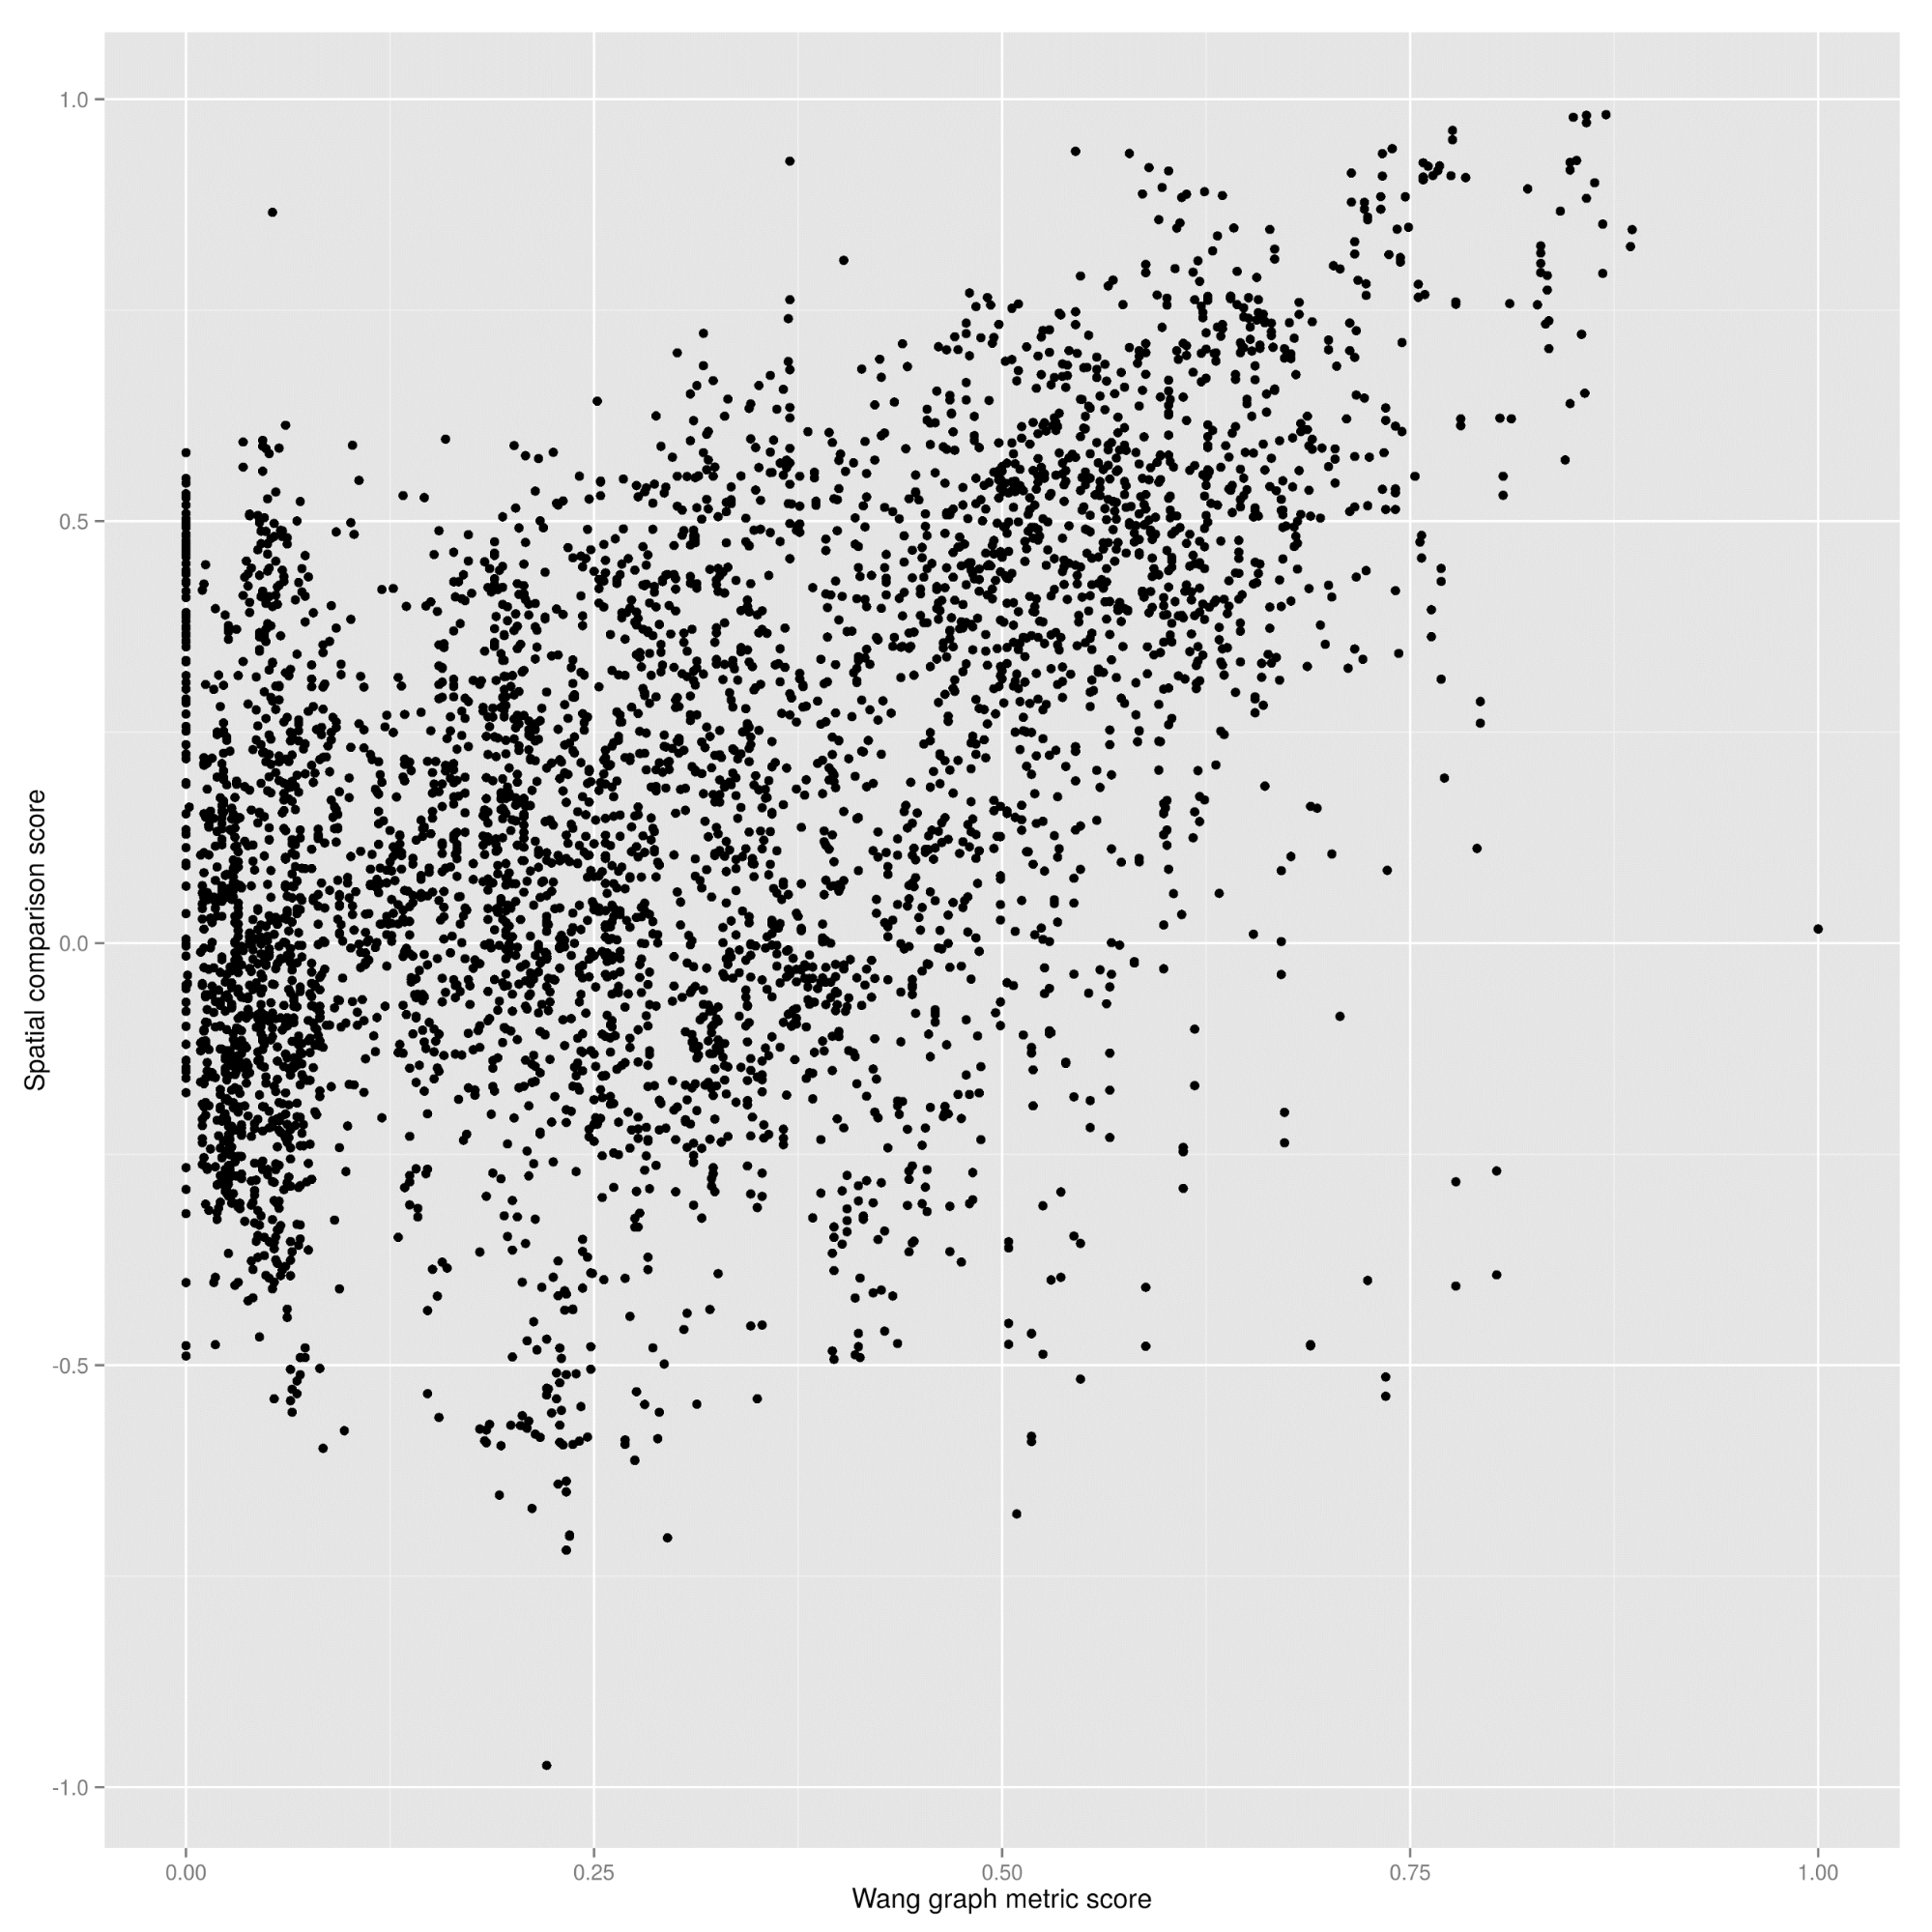
\includegraphics[width=15cm]{images/figure33.png}
\end{center}
 \caption{\label{fig:33} Comparison of semantic to spatial similarity. Semantic image
comparison is correlated with spatial image comparison (pearson score of
0.514 (95\% confidence interval = (0.499,0.53), p-value \textless{}
2.2e-16)) across all pairwise image comparisons. Task and contrast
specific RSA scores are included in \href{https://github.com/vsoch/thesis/blob/master/supplementary/chapter3/supp1_spatial_semantic_rsa_df.csv}{Supplementary data 3.2}.}
\end{figure}

\begin{table}[ht!]
\centering
\begin{tabular}{ | l | l | l |}
    \hline
    \textbf{Metric} & \textbf{Relation} & \textbf{RSA Score} \\ \hline
    katz  & part of & 0.537 \\ \hline
    ascos &  both & 0.527 \\ \hline
    wang &  kind of &  0.526 \\ \hline
    katz &  both &  0.526 \\ \hline
    ascos & part of	& 0.519 \\ \hline
    ascos & kind of	& 0.463 \\ \hline
    lhn & part of & 0.460 \\ \hline
    rss2 & part of & 0.460 \\ \hline
    katz & kind of &  0.458 \\ \hline
    inverse log weighted & part of	&  0.453 \\ \hline
    dice & part of & 0.401 \\ \hline
    cosine & part of & 0.382 \\ \hline
    dice & kind of & 0.371 \\ \hline
    jaccard & part of & 0.351 \\ \hline
    cosine & kind of & 0.320 \\ \hline
    inverse log weighted & kind of & 0.299 \\ \hline
    jaccard	& kind of & 0.286 \\ \hline
    rss2 & kind of & 0.263 \\ \hline
    lhn & kind of & 0.239 \\ \hline
    cosine & both & 0.100 \\ \hline
    jaccard	& both & 0.100 \\ \hline
    dice & both & 0.092 \\ \hline
    rss2 & both & 0.087 \\ \hline
    inverse log weighted & both & 0.086 \\ \hline
\end {tabular}\par
\bigskip
\caption{\label{table:table31} Relational Similarity Analysis (RSA) using graph similarity metrics for each of the kind of, part of, and combined ("both") relationships to compare pairwise semantic similarity of brain images to spatial similarity (ascos = "Asymmetric network Structure COntext Similarity", lhn = "Leicht-Holme-Newman"}.
\end{table}

\section{Discussion}

I have demonstrated that semantic comparison of images, both separately
from the voxelwise spatial data and in an encoding framework, is useful
for the classification of cognitive concepts, and contrasts from task
paradigms. The basic use case for this work is in a classification
framework, specifically providing a means to predict a cognitive concept
or contrast given a brain map, or a brain map from a cognitive concept
or contrast. Another use cases for this kind of framework would be to
assess the contribution of a new brain imaging result, possibly with
task or contrast unknown, to the entire set of concepts defined in the
ontology.

\subsection{Semantic image comparison in a classification framework}

Semantic labels to tag brain statistical maps with cognitive concepts to
drive a classification task performed well above chance (0.814 accuracy
compared to 0.47), giving strong support for the value of semantic
labels for image classification. This model is ideal in that it is a
multilabel procedure, as a single brain map can represent many cognitive
processes. While a robust exploration of different graph metrics to
optimize this classification is outside of the scope of this work, given
the demonstrated value of semantic labels, I see this question as a
primary interest for future work. Finally, the ability to predict brain maps based on semantic labels carries huge implications for reproducible evaluation of experimental results. If researchers can associate many experimental results (e.g., statistical brain maps) with a specific set of labels, it would be possible to pre-register a study about a cognitive paradigm, select terms that are expected to be represented in the map, and then generate a predicted map for the study outcome. Any experimental result produced can then be compared to this prediction. We could also flip the algorithm on its head and start with a whole-brain statistical map, and then predict labels to describe the map. While there are many good candidates for assessing the reproducibility of a result, an experiment could be called a replication given that it produces the same set of terms that are associated with one or more other experiments.

\subsection{Comparison of semantic to spatial similarity}

Representational similarity analysis shows that semantically-derived
comparison scores are well-comparable to spatially-derived pearson
correlation coefficients, the strongest indicator in this paper that
there is huge value in a semantically-based representation of brain
maps. The leading metrics, katz, ascos,and Wang, share the common feature that derives a score based on the structure of the graph, suggesting that assertions about relationships between cognitive concepts are an essential component to calculate semantic similarity of images. While the other metrics consider local neighborhoods, these methods take into account neighbors deeper into the graph, implying that there is value in a graph structure that has breadth as well as depth. Looking specifically at RSA scores for Wang derived by subsetting the comparison matrix to images tagged for unique cognitive concepts, we see that over half (0.58, 25/43) of the cognitive atlas terms had RSA scores exceeding 0.50, indicative of strong correlation of semantic and
spatial similarity. This result suggests that a subset of tasks and
concepts that are described in functional neuroimaging have distinct
spatial patterns of activation that can be identified in the algorithm
by comparing the set of images tagged with the term, versus those not.
This idea is supported by the observation that the weaker correlations
seem to be for tasks and concepts that are intuitively harder to
localize to distinct brain region(s), for example, ``theory of mind,''
and ``feature comparison,'' or ``negative feedback processing'' (RSA
scores = 0.32, 0.34, -0.06 respectively).

Interestingly, our result supports the idea that distinct, specific
labels (lower in the ontology tree) are more suitable for this task. For
example, the ``balloon analogue risk task (BART),'' is a complicated
task with many contrasts and concepts asserted to be measured by it (see
it's
\href{http://www.cognitiveatlas.org/term/id/trm_4d559bcd67c18}{entry in the Cognitive Atlas}), and combination of all images asserted to
belong to it produced semantic image comparisons that were not
comparable to spatial image comparisons, assessed by RSA (RSA
score=0.10). However, one of concepts that a contrast is asserted to
measure (visual object detection) was much more comparable (RSA
score=0.79). This suggests that semantic image comparisons may have
their highest value not on the higher level of an entire task, but on a
lower level, such as a contrast or concept, and this is logical because
more specific tags likely indicate image sets with less spatial
variance.

\subsection{Limitations}

Ontology development is a careful and slow process, and so analysis is
limited to describe the set of brain maps that were available in
NeuroVault database. I recognize that the size of this image set is
small, and that results will change as these image sets do. However,
growth in these databases is badly needed. The open idea of the
Cognitive Atlas is that participation is available to any researcher,
and the integration into NeuroVault and publicly available libraries
means ease of use to re-deploy methods to describe other datasets. The
terms and relationships can be fine-tuned over time, and are open for
discussion to the entire community. This original work provides a
reasonable first-go at this process to demonstrate that such a framework
is useful, and the result can be re-generated as the Cognitive Atlas and
NeuroVault databases are updated. Toward this aim, I want to encourage
researchers to upload statistical brain map results to the NeuroVault
database, tag these maps with contrast images from the Cognitive Atlas,
and continue to assist with development of the ontology at
\href{http://www.cognitiveatlas.org}{http://www.cognitiveatlas.org}.
I have developed a Github repo that uses continuous integration to
dynamically generate an updated visualization of concepts defined in the
Cognitive Atlas with tagged NeuroVault images to show these associations
(\href{https://github.com/vsoch/semantic-image-comparison-ci}{https://github.com/vsoch/semantic-image-comparison-ci}).

\section{Conclusion}

I have performed simple, intuitive image comparison analyses using
openly available data and methods that can be reproduced as the
Cognitive Atlas and NeuroVault databases grow, and demonstrated that
such a comparison is comparable to the more commonly done calculation of
spatial similarity. I am hopeful that these methods and promising
results will provide incentive to continue the study of semantic
information to assess similarity of brain statistical maps.



\chapter{Summary and conclusions}

In this dissertation, I have reviewed convergent methods for spatial and semantic image comparison of brain imaging data, and provided a direct means to map cognitive processes onto statistical brain maps. I start with a body of work to better define standard comparison
methods in the domain of cognitive imaging, presenting work to identify
optimal methods for spatial comparison of whole-brain statistical maps
(Chapter 2). This is the ``spatial'' component of this dissertation
work, and is a powerful example of comparison methods that are in line
with the goals of the researcher performing a meta-analysis. Chapter 3
addresses the ``semantic'' feature space, demonstrating clear value in integrating
standard terminology about cognitive processes to drive image comparison
for meta-analysis.

Integrated into these tools I have deployed my research findings by way
of methods and prototypes that have real extendable, usable, value.
Through methods and tools, this work sets up a basic framework for
researchers to conduct meta-analysis to assess the replication of a brain statistical
map. This is essential to better synthesize and grow our understanding of the function of the human brain to aid the mental health crisis. It was not known before this work if semantic annotations had value for the assessment of similarity of whole brain statistical maps. This work sets up rationale
and infrastructure for the growth of an entire new domain: applying
methods from graph theory not on the imaging data itself, but on the
semantic annotations associated with it. These semantic annotations are
reliably linked to the experiments by way of the Cognitive Atlas,
bringing badly needed standardization for development and deployment of
these paradigms.

Underlying this work is my deepest desire to push forward the need for
academic software developers and optimal methods and infrastructure for reproducible
science. Building tools that are integrated with sound methods, and that are easy to use, is essential for data science to help the human condition. It is with great anticipation that I look forward to pursuing this path to build tools that have impact in the next stage of my career. 

\appendix

\chapter{Standardizing behavioral experimentation}

In this chapter, I describe development of a novel infrastructure to
develop and deploy experimental paradigms (\cite{Sochat2016-pu}). I begin with a description of the goals of this research, followed
by a detailed technical report of all components of the software.

The Experiment Factory is an open source
framework for the development and deployment of web-based experiments (\cite{Sochat2016-pu}).
The modular infrastructure includes experiments, virtual machines for
local or cloud deployment, and an application to drive these components
and provide developers with functions and tools for further extension. I
have released this infrastructure with a deployment
(\href{http://www.expfactory.org}{http://www.expfactory.org})
that my lab, the Poldrack Lab, is currently using to deploy a set of
over 80~standardized~web-based experiments to Amazon Mechanical Turk. By providing open source tools for both deployment and development, this
novel infrastructure holds promise to bring reproducibility to the
administration of web-based experiments, and accelerate scientific
progress by providing a shared community resource of psychological
paradigms.

\section{Experimental definition and capturing of behavior}

Psychological science is concerned with the study of behavior, and
logically a behavior cannot be studied without some kind of measurement.
Psychometric theory \cite{noauthor_undated-oa} provides
a conceptual definition for best practices in measuring observed
behavior, and extending to a numerical framework to allow for
statistical analysis of behavior. Typical avenues for collecting
behavioral metrics might include asking an individual about a cognition
or experience (self-report), directly observing a phenomenon
(observational or field research), or by direct measurement or control
(experimental). While historical assessments of behavior might involve
verbal or written responses (self-report) or manual counting of
frequency or measurement of a desired behavior, modern assessments tend
to be digital, typically delivered on the web or via a digital screen.
These experimental paradigms form the basis of modern study of behavior.

\subsection{Modern behavioral experimentation}

Experimental paradigms are central to psychological science, because
they provide the primary means by which we quantify human behavior.
Ideally there would be a coordinated effort to develop and deploy these
paradigms, but unfortunately there is no openly available, extensible
coordinated effort, and thus behavioral datasets tend to be small, and
not directly comparable across studies. The technology available is also
limited; while several frameworks have been developed~for specific steps
in the experimentation process (e.g. jsPsych \cite{De_Leeuw2015-zw}
for experiment creation, Psiturk \cite{McDonnell2012-ns} for
deployment), these tools require expertise with programming or the
command line, and lack an integrated framework. Additionally, there is
currently no large, open repository of paradigms that can serve as a
resource and standard for the field. Without such a resource, individual
labs must either spend unnecessary time time coding tasks, or pay for
commercial products that provide a battery of psychological assessments.
The former complicates replication and~interpretation when reportedly
identical paradigms differ in their implementation.The latter
hamstrings~research by providing a particular set of tasks that cannot
be extended or modified and that are limited to laboratories with
sufficient resources to pay for them. The success of psychology requires
adoption of modern technology, including instant online access to
deploying surveys (e.g., http://www.surveymonkey.com, http://www.qualtrics.com).
integration with social media (e.g., Facebook, Twitter), and a general
movement towards a fast, broad collection of data \cite{Mason2011-fz}.

A promising trend in this disorganized landscape is the growth of
browser-based experimentation, such that behavioral paradigms are
delivered online or offline through a web browser. ~While some toolboxes
are limited to running with specific software \cite{Schneider_W_Eschman_A_and_Zuccolotto_A2012-fe,Brainard1997-rq},
there is clear move towards delivery of experiments over the web using
platforms like Amazon Mechanical Turk. The use of the web necessitates a
move to~standard web technologies including JavaScript \cite{Foundation-jqueryorg_undated-ra},
HTML, and CSS \cite{noauthor_undated-ov,noauthor_undated-qj}.
The primary benefit of web-based experimentation is that experiments can
be delivered across platforms (e.g., computers, mobile phones, tablets,
fMRI projected screens), and environments (controlled and uncontrolled
settings). Companies have noticed this trend, and there are a number of
pay-for-service products available \cite{noauthor_undated-fh,noauthor_undated-rv,noauthor_undated-el}.
These products are not ideal for researchers who generally desire
transparency and control over their experiments, and commercial products
are ill-suited for the development of a field-wide repository of shared
experimental implementations. The development of an open-source
equivalent, on the other hand, would meet these requirements.

A wide range of standard infrastructures are in development to help with
this task. ``Just Another Tool for Online Studies'' (JATOS) provides
infrastructure to set up a local or server-based set of JavaScript
experiments with a corresponding database, but does not address the
issue of standardizing or re-using paradigms \cite{Lange2015-dd}.
The Project Implicit Framework (PIP) \cite{noauthor_undated-fd} is
a modular framework that also deploys JavaScript experiments, but
requires significant expertise to develop and set up components of the
application. Psiturk \cite{McDonnell2012-ns} is
a Python-based web framework (based on the Flask micro-framework) that
researchers can use to develop experiments and deploy on Amazon
Mechanical Turk, but is limited to that implementation, and requires
researchers to develop their own paradigms. Finally, Tatool is a
web-based tool for researchers to create and run experiments, offering
modern and accessible experiment generation and analysis. While Tatool
is easy to use and a great contribution to open-source experiment
technology, it does not provide standardization to the development of
experiments, sharing and development of a common resource, or
integration with existing deployment options (e.g., Psiturk) \cite{Makin2016-xi}.

\subsection{Open source infrastructure to measure behavior}

Open source software for creating experiments has relied upon a small
number of libraries and software: Psych Toolbox \cite{Brainard1997-rq} (Matlab),
psychopy \cite{Peirce2007-qr}, jsPsych \cite{De_Leeuw2015-zw} (JavaScript).
Within this current system, sharing of code is infrequent, documentation
tends to be sparse, formal testing is almost nonexistent, and paradigms
are passed between labs and PIs like protected family heirlooms. The
detriments to the research process are extensive. First, independent
development of standard paradigms by multiple individuals leads to
redundancy of effort and increases the probability of coding and
conceptual errors in task design. Without open sharing of the
experiments, it is not clear if different results in an analysis are due
to a true effect, or an artifact of the different implementations.~In
addition, such practices slow the adoption and vetting of new paradigms
once they are published, since implementation of a new paradigm either
requires coding it anew or acquiring it from the original lab, both of
which delay reproduction and extension of the original work. There is
also the potential that untested code can propagate errors across
multiple laboratories. Finally, this potpourri of solutions fails to
include any kind of description about how the data being collected links
to cognitive processes of interest, a goal that might be aided by
ontology.

\section{The Experiment Factory}

An essential and often overlooked feature of research workflow is the
distinction between developer and user. A developer is a researcher
interested in creating experimental paradigms and infrastructure, while
a user simply wants to use the paradigms. While some researchers aim to
dig deep into the code for an application, others simply want to use it, and a successful infrastructure must serve both. Toward this aim, the
Experiment Factory employs a modular strategy, providing separate
components (Github repositories) for experiments, battery, and
deployments (see The Experiment Factory Infrastructure),
and allows researchers to deploy experiments into current tools that
researchers already find useful (e.g., Psiturk, see Table~\ref{table:table43} for Glossary
of terms), and under different likely scenarios like not having access
to an internet connection, or needing to save data to a private
database. First I will outline some use case scenarios to describe the
motivation behind this work, followed by an outline of the
infrastructure in more detail.

\subsection{The Experiment Factory Use Cases}

\subsubsection{Deployment of Experiments}
The Experiment Factory aims to offer both flexibility and structure. A
researcher has complete control over the deployment environment (local
or cloud), along with the infrastructure used for the deployment (see
The Experiment Factory Infrastructure). Under any
circumstance, the researcher has complete control over the set of
experiments that are selected, and the resulting data are provided in
several output formats. For this thesis, I will walk through several use
cases. When I refer to a module such as ''experiments,'' I am referring
to a Github repo, and more information is available about these
components in the second part of this chapter.

\paragraph{Local Deployment of Experiments}

The most basic use case is when a researcher wants to run participants
locally through the paradigms already included in the experiments
module. This approach is easily accomplished using the expfactory
command line tool (Section 4.2.1 The Experiment Factory Software). Using
the tool, a researcher can, in one line of code, select experiments,
define a participant unique ID, and bring up a web interface to deploy a
set of connected experiments called a ``battery'':

expfactory --run --experiments stroop,nback --subid UID001

In the case that the user wants to save a static folder to run later,
the argument ``--generate'' can be used in a similar fashion. While the
default behavior is to use the latest experiments and battery templates
from the repositories, a researcher can ensure that experiments and
battery code remains constant by saving (cloning) the repositories to a
local machine, and providing the paths to the folders as arguments to
the tool (see the docs at expfactory.readthedocs.org for details). The
data are downloaded to the local machine directly in the browser after
the experiment completes, and named according to the participant unique
ID.

\paragraph{Deployment of Experiments using Psiturk}

The Psiturk infrastructure is a well-developed platform for deploying
experiments on Mechanical Turk. Due to its substantial user base and
documentation, it was imperative that the experiments be easily
deployable to Psiturk. Using the expfactory command line tool without
any arguments:

expfactory

a user can open up a web interface to choose experiments, a database
specification, and a deployment. After selection of these variables,
either a folder or file to run a virtual machine is provided to the
user. This functionality is also possible using the command line tool
with the command:

expfactory --generate --experiments stroop,nback --folder /home/output

\paragraph{Local Modification of Experiment or Battery}

Researchers may want to use the experiments included in the experiments
module as a ``base paradigm'', but make modifications for their own
purposes (e.g. change the stimuli images, increase the trial length).
Similarly, researchers may want to supplement the paradigms available
with their own experiments. If a set of experiments have already been
downloaded as a set of folders, modifying a paradigm simply requires
changing the files in a specific experiment folder. While this currently
requires some JavaScript coding knowledge, modification of a restricted
set of experiment variables through variables in the configuration file
of an experiment (Table~\ref{table:table41}) will be implemented in the future. \newline

\begin{table}[ht!]
\centering
\begin{tabular}{ | l | l | l | p{3cm} |}
    \hline
    \textbf{Field Name} & \textbf{Requirement Level} & \textbf{Rationale} & \textbf{Example} \\ \hline
    name & not required, warning & \shortstack[l]{descriptive label\\ of experiment} & Antisaccade \\ \hline
    run & \shortstack[l]{required,\\ not valid without} & \shortstack[l]{scripts required \\ for the experiment \\ to run } & \shortstack[l]{experiment.js \\ style.css } \\ \hline     
    exp\_id & \shortstack[l]{required,\\ not valid without} & unique identifier & antisaccade \\ \hline
    cognitive\_atlas\_concept\_id & not required, warning & \shortstack[l]{mapping of experiment \\ to cognitive concepts \\ it measures} & trm\_4b1968619b00b \\ \hline
    contributors & not required & \shortstack[l]{credit and source \\ of help} & \shortstack[l]{Ian Eisenberg \\ Vanessa Sochat \\ Zeynep Enkavi} \\ \hline
    time & \shortstack[l]{required,\\ not valid without} & \shortstack[l]{run time in \\ minutes} & 8 \\ \hline
    experiment\_variables & not required & \shortstack[l]{variables for \\ allocation of \\ credit or reward } & reaction\_time \\ \hline
    reference & not required, warning & \shortstack[l]{full documentation of \\ paradigm } & doi:10.1006/... \\ \hline
    notes & not required & \shortstack[l]{additional \\ information to \\ capture} & should not wear glasses \\ \hline
    publish & \shortstack[l]{required,\\ not valid without} & \shortstack[l]{ready for  \\ deployment} & True \\ \hline
    template & \shortstack[l]{required,\\ not valid without} & \shortstack[l]{experiment \\ library base } & jspsych \\ \hline
\end {tabular}\par
\bigskip
\caption{\label{table:table41} The fields required in the standard ``config.json'' for an Experiment Factory Experiment. The definition of files and and a template are essential to validate the function of the experiments. The examples for each field above are limited and not in JSON, full config.json are available for inspection in the experiment folders (\href{https://github.com/expfactory/expfactory-experiments}{https://github.com/expfactory/expfactory-experiments})}.
\end{table}

\subsection{Development of Experiments and Infrastructure}

The Experiment Factory uses an open source development strategy, meaning
that all code is publicly available on Github (\href{http://www.github.com/expfactory}{http://www.github.com/expfactory}), and contributions are made to any of
the code bases via forking of repositories and pull requests. Full
documentation about this process is available (\href{http://expfactory.readthedocs.org/en/latest/development.html\#contributing-to-code}{http://expfactory.readthedocs.org/en/latest/development.html\#contributing-to-code}).
The code base has been developed and tested on Linux (Ubuntu) and Mac
OS.

\subsubsection{Experiment Development}
Contributing a new experiment constitutes adding a new folder to the
experiments repository that meets the minimal requirements for
expfactory (i.e. including a JavaScript file to run the experiment, and
a configuration file to specify meta-data). Additional script and style
files, along with images, sound, or other files necessary for
deployment, are optional. An experiment template is provided for
researchers to start with, and a recommended strategy is to copy and
make modifications to a similar experiment that already exists.
Development of an experiment means some familiarity with JavaScript and
HTML/CSS, and ability to collaboratively work on Github. Descriptions
about the required variables for the configuration file are provided
(Table~\ref{table:table41}). To test experiments, the user has several options. The
Experiment Factory software command line tool can be run from within any
experiment folder to open up a web browser to test a single experiment
manually with ``expfactory --preview,'' to test a single experiment with an experiment robot using ``expfactory --test,'' or to validate the configuration file with ``expfactory --validate.''

See full documentation at \href{http://expfactory.readthedocs.org}{http://expfactory.readthedocs.org}.

\subsubsection{Documentation and Infrastructure
Development}

Infrastructure and methods are useless without proper documentation. The
Experiment Factory uses the sphinx documentation tool, served with the
Experiment Factory Github repository, meaning that it is built
automatically when the code base is updated. This documentation standard
uses restructured text syntax (rst)
(\href{http://docutils.sourceforge.net/rst.html}{http://docutils.sourceforge.net/rst.html}). A set of pages have been
written to supplement the functions that the module provides, and also
provided is documentation for how to contribute to documentation (\href{http://expfactory.readthedocs.org/en/latest/development.html\#contributing-to-this-documentation}{http://expfactory.readthedocs.org/en/latest/development.html\#contributing-to-this-documentation}).
Contributions for any of the Experiment Factory components from the
larger community are welcomed and encouraged.

Complete tutorials and further details are provided in our development
documentation \newline
(\href{http://expfactory.readthedocs.org/en/latest/development.html}{http://expfactory.readthedocs.org/en/latest/development.html})

\section{The Experiment Factory Infrastructure}

This section is intended for more technical readers and those interested
in development of the Experiment Factory modules, and a Glossary of
terms (Table~\ref{table:table43}) is provided to explain more technical jargon. The
modular strategy of the Experiment Factory infrastructure means
providing separate Github repositories for experiments, skeletons for a
sequence of experiments (a ``battery'' of experiments), and deployments.
The Experiment Factory aims to be agnostic when it comes to deployment,
and to provide support for the current infrastructures that researchers
find useful to deploy their experiments. For example, experiments can be
easily deployed into a folder structure to plug in to Psiturk, either
locally on a virtual machine, or served locally to study participants
without an internet connection. These static components are separate
from the software that drives integration of the components, and all
components and software are completely open source (Github, RRID:SCR
002630), allowing for collaborative specialization. A researcher
interested in developing an experiment need only add a new paradigm to
the experiments repository, and it will be available to all applications
that use the Experiment Factory. A researcher primarily interested in
further developing the software can do so without needing to touch
static components. Currently the entire system is available for
deployment by any researcher, either locally or using a cloud server;
ultimately, the Poldrack Lab also hopes to provide a hosted version as a
service open to all researchers. An overview of the infrastructure is
included in Figure~\ref{fig:41}.

\begin{figure}[ht!]
\begin{center}
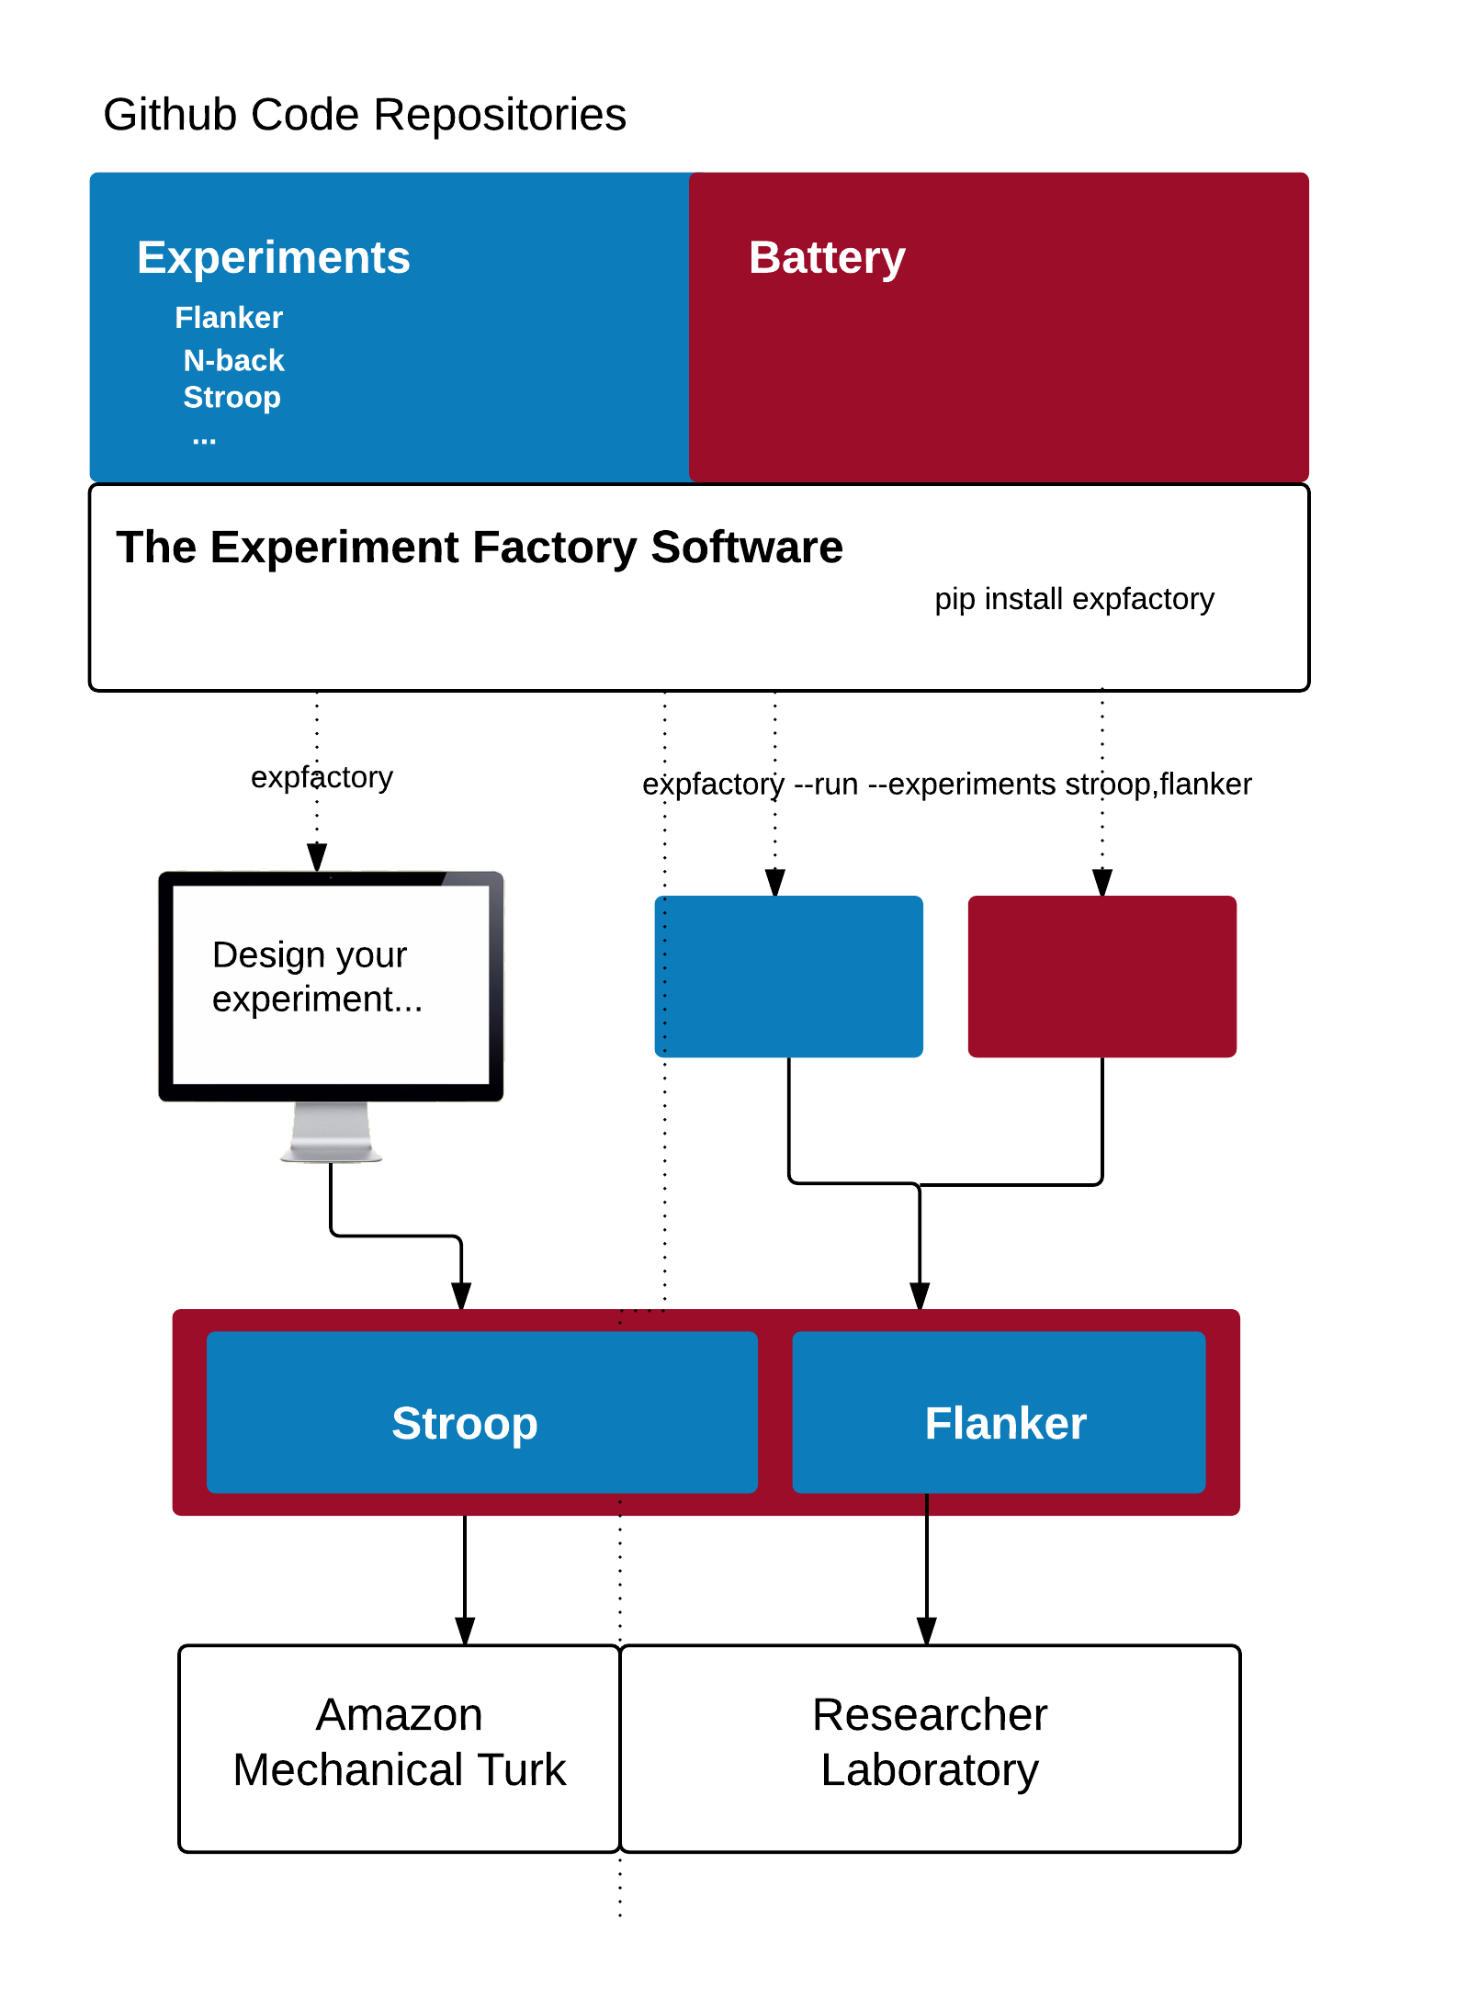
\includegraphics[width=10cm]{images/figure41.png}% This is a *.jpg file
\end{center}
\caption{\label{fig:41} The Experiment Factory Core includes Experiments, a battery skeleton, and the software, all of which are openly available on Github. Installation of the Experiment Factory tool allows a researcher to run a sequence of experiments on the fly (right panel) or to generate a local folder or virtual machine to deploy experiments to Amazon Mechanical Turk using Psiturk (left panel).}
\end{figure}

\subsection{The Experiment Factory Software}

The controller of the Experiment Factory is the Experiment Factory
Python software \newline (\href{https://github.com/expfactory/expfactory-python}{https://github.com/expfactory/expfactory-python}) that
provides functions for working with components, testing and validating
experiments, and generating the final battery output based on the users
specifications. For example, after installing this tool, a researcher
can, in one line, specify experiments and an optional subject unique id,
and a browser opens with the rendered battery. Behind this simple
functionality, the software is obtaining experiment and battery files
from Github, validating the experiments, and parsing configuration files
to render the users selected experiments into the correct HTML syntax.
The finished HTML syntax, along with experiment code and static files,
is saved in a temporary directory, and a web server is opened to run the
experiments as a sequence.

The tool is also useful to developers in that any function in the
software can be used in an external application. By way of being a
Python Flask application (see Table 3 for Term Glossary), running the
executable also provides a RESTful API to serve experiment meta-data,
which can be deployed in a local or cloud server environment. The
application is easily installed with a package manager (\href{https://pypi.python.org/pypi/expfactory}{https://pypi.python.org/pypi/expfactory}), and developers can
collaborate on this software to develop additional functions for use
with the entire family of Experiment Factory components.

\subsection{The Experiment Factory Experiments}

The Experiment Factory Experiments
(\href{https://github.com/expfactory/expfactory-experiments}{https://github.com/expfactory/expfactory-experiments}) are the core of
the infrastructure: at the time of this publication there are more than
80 coded experiments available for deployment. Each experiment is a
single folder in the Github repository that contains a data structure
(config.json) file with a standard set of key-value relationships that
provide meta-data on the experiment, and allow for its deployment. Table
1 provides an overview of fields, requirements, and examples, each of
which is checked before an experiment is considered valid. For example,
the definition of files necessary to run the experiment is essential for
the expfactory-python tool to validate and deploy the experiments, and
the definition of variables makes them available to the higher level
applications. Each experiment is given a unique identifier, the
``exp\_id'' variable, that coincides with the folder name in the Github
repository. The boolean field ``publish'' makes it possible to quickly
disable deployment of a particular experiment, and the fields
``reference,'' and ``contributors'' are important to allocate credit to
developers. Finally, fields related to the Cognitive Atlas \cite{Poldrack2011-jp} allow
for a common place to document details and references for the
experiment, and define an experimental paradigm in an ontology that
makes assertions about the cognitive concepts measured by the task. This
means that a comparison can be made between tasks with regard to the
processes or phenomena that are measured (e.g., finding all tasks that
are thought to measure the construct of ``response inhibition''). The
``template'' field specifies the library (e.g., JavaScript functions)
that the experiment is coded in, such that the deployment template will
be customized for the library. Although the initial release includes
experiments coded using jsPsych, a Javascript library that simplifies
experiment creation, the modular framework and specification of this
template means that the infrastructure is ready to be extended to any
web-based technology. This is extremely important to allow for
development of experiments using the most up-to-date web-based
technologies.

\subsection{Experiment Factory Battery}

The experiment-factory Battery
(\href{https://github.com/expfactory/expfactory-battery}{https://github.com/expfactory/expfactory-battery}) is a simple skeleton
into which Experiment Factory experiments can be deployed as a cohesive
set of experiments, called a ``battery.'' The battery comes with a set
of standard JavaScript and stylesheets common across the templates
(e.g., jsPsych), meaning that code that is consistently re-used across
paradigms can be added to this repository. The design of the battery
allows immediate deployment to multiple infrastructures, including
Psiturk (locally or via a virtual machine), to a local machine to run on
the fly, or a Django (RRID:SCR 012855) application that can be served
locally or on a server (expfactory-docker). This Django application
drives the (www.expfactory.org) interface.

\subsection{Experiment Factory Docker}

One of the main goals of the Experiment Factory is to provide an ability
to deploy experiments and collect data without any knowledge of
programming, databases, or a command line. Under this requirement,
download of a command line application is one step too many, and for
this reason we developed a container-based application running at
expfactory.org. The Experiment Factory Docker is a set of containers
that serve a Django application that can be run locally or on a server
to provide a login interface for labs to run experiments locally, or
from the cloud. The application supports both http and https (secure
connections). Although the functionality is not exposed to the general
user, the application is also configured to deploy experiments to Amazon
Mechanical Turk. The ease of deployment is thanks to Docker, an emerging
container-based architecture that allows for development and deployment
of applications in Linux containers (http://www.docker.com). Docker
Compose (\href{http://docs.docker.com/compose}{http://docs.docker.com/compose}) is a controller for running
multi-container applications such as the Experiment Factory, which uses
separate containers for a nginx web server (nginx-proxy), a postgresql
database (postgres), a Celery job manager worker to run time- intensive
jobs (worker), a database for the jobs (redis), and the core application
(expfactory), and protocol (uwsgi) for serving the application. An
overview of these containers, along with the images on the Docker Hub,
are provided in Table~\ref{table:table42} and Figure~\ref{fig:42}, and a summary of terms are
provided in a glossary (Table~\ref{table:table43}). For a more secure deployment (e.g.,
expfactory.org), it is recommended to link the application to a separate
database with an encrypted connection over running the postgres
container on the same server. Django (\href{https://www.djangoproject.com/}{https://www.djangoproject.com/}) is
a Python-based framework that comes with a strong user base,
well-developed plugins for authentication, security, and a backend
database, and if desired, the Django application could be run
independently from Docker.

\begin{figure}[ht!]
\begin{center}
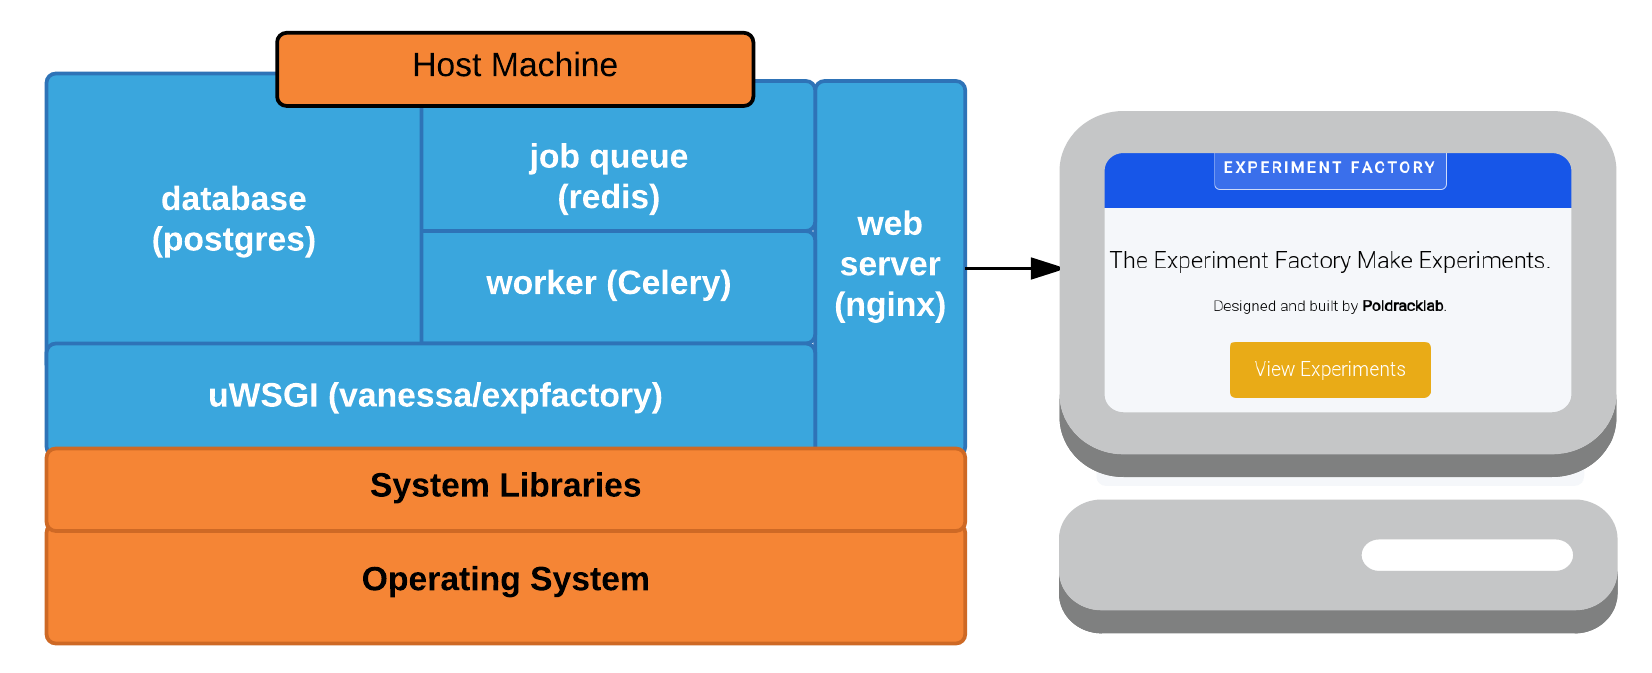
\includegraphics[width=10cm]{images/figure42.png}
\end{center}
\caption{ \label{fig:42} Expfactory-docker includes the main application container (expfactory), a database for storing application data (postgres), a job queue (redis) and worker (Celery) for running computationally intensive tasks, and a web server (nginx) to serve the application to the web. \newline \newline}
\end{figure} 


\begin{table}[ht!]
\centering
\begin{tabular}{ | l | l | l |}
    \hline
    \textbf{Container Name} & \textbf{Purpose} & \textbf{Image} \\ \hline
    expfactorydocker\_uwsgi\_1 & \shortstack[l]{Django application, and \\ uwsgi protocol for serving it} & expfactory \\ \hline
    expfactorydocker\_db\_1 & \shortstack[l]{postgresql database for Django application \\ and storing results} & postgres \\ \hline     
    expfactorydocker\_nginx\_1 & ``Engine X'' web server & nginx \\ \hline
    expfactorydocker\_worker\_1 & celery worker for running tasks & expfactory \\ \hline
    expfactory\_redis\_1 & \shortstack[l]{redis database for tasks, serialized \\ as JSON} & redis \\ \hline
\end {tabular}\par
\bigskip
\caption{\label{table:table42} Docker Containers utilized in expfactory-docker to run the \href{www.expfactory.org}{www.expfactory.org}. The container images are downloaded from the Docker hub. The container image ``expfactory'' corresponds to the expfactory-docker repository, and is built automatically from this source. For a more substantial deployment, the database can be external to the instance (eg, Amazon RDS) with an encrypted connection.}
\end{table}

\begin{table}[ht!]
\centering
\begin{tabular}{ | l | l |p{5cm} |}
    \hline
    \textbf{Term} & \textbf{Definition} \\ \hline
    Amazon Mechanical Turk (MTurk) & \shortstack[l]{a platform provided by Amazon Web \\ Services to allow individuals (Requesters) to \\ deploy ``human intelligence tasks,'' \\ or computer-based tasks that are \\ difficult for computers, for \\other people to complete.} \\ \hline
    battery & \shortstack[l]{a set of experimental paradigms presented in \\ sequence to a study participant } \\ \hline
    Celery & \shortstack[l]{a distributed task queue to allow for \\ scheduling of function executions on a server} \\ \hline
    Continuous Integration & \shortstack[l]{the continuous testing of functions in code \\ whenever a change is made to ensure \\functionality does not break with changes} \\ \hline
    Docker & \shortstack[l]{a container-based infrastructure to package \\an entire software environment (code, system \\libraries, files) for consistent deployment on \\different computers} \\ \hline
    Docker Compose & \shortstack[l]{A tool for specification of how different\\ Docker containers work together to build an \\application with multiple containers} \\ \hline
    Django & \shortstack[l]{a Python-based web framework that makes it\\ easy to extend python-based functions into\\ the web browser } \\ \hline
    Flask & \shortstack[l]{a Python-based micro-framework with less \\stringent requirements than Django to extend \\python-based functions into a web browser} \\ \hline
    jshint & \shortstack[l]{a code analysis tool to check static (not\\ running) JavaScript code for common errors} \\ \hline
    jsPsych & \shortstack[l]{a JavaScript library for creating and running\\ behavioral experiments} \\ \hline
    Psiturk & \shortstack[l]{a Flask application to deploy \\web-based experiments to \\Amazon Mechanical Turk} \\ \hline
    Selenium & \shortstack[l]{A tool to allow for programmatic control of \\web browsers} \\ \hline
    Sphinx & \shortstack[l]{a documentation generation language for \\Python} \\ \hline
    Redis & \shortstack[l]{An open source data structure store that can\\ easily handle storage of different data\\ structures for use with other applications} \\ \hline
    uWSGI & \shortstack[l]{a tool to easily deploy web applications,\\ including load balancing, process and task\\ management, and monitoring} \\ \hline
\end {tabular}\par
\bigskip
\caption{\label{table:table43} Glossary of terms for technical jargon, software, and tool references.}
\end{table}

\subsection{Experiment Factory VM}

Deployment of a battery to a virtual machine, whether locally or to the
cloud, is made possible by the expfactory-vm repository. This repository
contains Vagrantfiles that can be used with the Vagrant software
(http://www.vagrantup.com) to run a local Virtual Machine, or one
deployed via Amazon Web Services. The files can be used ``as is'' to
deploy a battery with all experiments, or generated through the
expfactory-python executable to allow a user to define a custom set of
experiments.

\section{Design and Implementation Choices}

\subsection{Modular Framework for Open Science}

The choice to use Github, and to separate the Experiment Factory into
its underlying components (experiments, battery, docker, documentation,
and vm) was a specific choice to allow specialization and collaboration
in development. Github offers version control, management of code, and
collaboration between teams, along with features such as reporting
issues, discussing changes, and managing documentation. All versions of
code are archived, and multiple features can be worked on simultaneously
by any researcher with an internet connection. Github also provides
Continuous Integration, or automatic testing of code, both for the
experiments and expfactory-python, discussed next.

\subsection{Software testing for the Experiment Factory}

An essential component of software development is continuous testing of
all functions whenever changes are made to the software in the case that
a change breaks an essential functionality. This task, called Continuous
Integration, can be done automatically when new changes are proposed to
code on Github with services like CircleCI ((\href{https://circleci.com/}{https://circleci.com/}) and
Travis (\href{https://travis-ci.com/}{https://travis-ci.com/}). 
The base software to run the Experiment Factory (expfactory-python) is consistently tested in this fashion, however a significant challenge in the development of this
infrastructure was ensuring functionality of the experiments themselves.
An error in an experiment at run-time would end a battery, and must be
avoided at all costs. Toward this goal, the Experiment Factory has
several strategies for testing experiment code in a Continuous
Integration environment. First, testing of experiments includes using
jshint, a JavaScript quality tool, to parse experiment code files for
static errors. The validation of experiments config.json data structures
also occurs in the Continuous Integration environment, as does testing
the experiments at run-time. This is made possible by using an automated
web browser, selenium (\href{http://www.seleniumhq.org}{http://www.seleniumhq.org}), controlled by python functions from expfactory-python that respond to the stimuli, akin to
running an experiment robot. When experiments are modified, the
experiment robot is run over these changed experiments to ensure no
run-time errors, triggering an error to fail the Continuous Integration
tests if any errors are found. During this process, developers can
discuss changes and issues using the standard forums for reporting
issues and discussing development that are provided by Github. This
collaborative coding environment has been an essential component for our
group to develop, pilot, and discuss the application. Using version
control was an essential factor for the Experiment Factory to follow the
vision of reproducible science.

\subsection{The Cognitive Atlas}

The Cognitive Atlas \cite{Poldrack2011-jp} is
an ontology that represents current knowledge about cognitive science.
Integration of standard terms to describe the tasks, and consequently,
the cognitive concepts that are measured by them, allows for researchers
to map all experiments into a common space, and use a common language to
describe the behavior and phenomena that are being measured. This means
that, for example, a researcher can quickly find experiments that are
asserted to measure ``risk seeking,'' and such a feature is not only
important for definition of these experiments, but also for
meta-analysis and reproducible science. The expfactory.github.io
experiment portal, along with documentation and testing of experiments,
offers a view to browse experiments based on the cognitive concepts that
are measured, as defined in the Cognitive Atlas. Mapping experiments to
the Cognitive Atlas and making assertions about the cognitive concepts
measured by the experiments is powerful in that it allows researchers to
select paradigms based on the specific cognitive functions that they are
thought to measure.

\section{Discussion}

I have developed the Experiment Factory with a vision of open,
collaborative science. The modular application is flexible to be used by
both developers and researchers without development experience, and
structured so that experiments must follow guidelines that will make
them extendable to multiple frameworks. I have integrated the Cognitive
Atlas as a way to provide structure in making assertions about what the
experiments measure - any experiment tagged with a unique identifier in
the Cognitive Atlas can immediately be compared to other experiments on
the level of the cognitive concepts. While I am optimistic about this
approach, there are several limitations.

\subsection{Software Versioning}

A key challenge with any kind of deployment of this nature is software
versioning. For example, the current experiments and battery are up to
date with the most recent version of the JsPsych library, and upgrading
this software would require developers to update current experiments.
Thus, a standard in software development is to instill that care is
taken to make available different versions of the software to support
legacy implementations. Significant new releases of dependencies can be
integrated when the developer community decides they are needed, and
these same developers take responsibility for ensuring proper function
of components. This is the rationale for Continuous Integration to run
tests of the function of software, which has been implemented and
provided by way of CircleCI (www.circleci.com) integration with Github.

\subsection{Ontology Development}

The Cognitive Atlas may not contain every experimental paradigm that
would be desired, and so it might be required for a researcher to add a
new experiment, extend documentation on an already defined experiment,
or better develop the assertions about the cognitive concepts that the
task measures. Ontology development is an ongoing process.

\subsection{Operating Systems and Browsers Supported}
The Experiment Factory experiments have been tested fully on Chrome and
Firefox browsers running on Linux and Mac OS systems. While there is a
plan to develop a desktop application that will have cross platform
support (i.e., including Windows), this desktop application is not yet
available. In the meantime users are encouraged to use the tools on
Linux and Mac OS, in Chrome or Firefox, and to use a virtual machine for
support on Windows systems.

\subsection{Future Development}

The Experiment Factory aims to keep the various components and
experiments modern. I believe that the same technology available and
used in industry should be extended to researchers, and for this reason
have chosen the current approach that uses modern technologies such as
Docker, Amazon Mechanical Turk, and Amazon Web Services. Coinciding with
this goal, I see a potential opportunity to deploy experiments via
social networks such as Facebook, and have plans to develop this
ability. I have also developed an easy deployment of a text file with
survey questions to allow easy deployment of browser-based surveys
(expfactory-surveys). This is an important contribution as I believe the
JsPsych framework is an overly complex solution for the administration
of simple form data. I see great potential in the development of
experiments beyond the jsPsych framework, and have extended a
collaboration to the lab of Vinod Menon at Stanford to use the framework
to deploy the first browser-based game. Given the open nature of this
work, I encourage and invite all researchers to join in the development
of experiments, battery template, and deployment infrastructures.

\section{Conclusion}

The Experiment Factory is a modular infrastructure that applies a
collaborative, open source framework to the development and deployment
of psychology experiments. I am pleased to offer this as a resource for
the larger community, and excited to further the development toward the
needs of users toward a vision of reproducible science.

\chapter{Visualization Best Practices for Complex Brain Connectivity Data}

In this chapter, I discuss challenges and best practices for visualization of brain connectivity. Data visualization in statistics for highly dimensional and complex data is essential for discovering patterns, generating hypothesis, and developing subsequent models of natural phenomena.  For the field of brain imaging, this task presents numerous substantial challenges.  For instance, highly complex data must be processed and presented in a manner that is intuitive and transparent to the viewer, and the visualization itself must strike a fine balance between revealing the data’s inherent complexity and providing an easily digestible abstraction.  Further, the visualization strategy must be integrated with tools that enforce standards for data format. Finally, for ease of use, the visualization must be quick and easy to navigate.  This goal has not been achieved for functional connectivity data, which is a burgeoning field of neuroimaging that attempts to map the dynamic interactions between neural regions. Unfortunately, the standards for visualization of such functional networks are trapped in a dated practice of producing static, and often biased, figures, thus hampering effective scientific communication.  Here I embrace this substantial opportunity to bring cutting-edge web technology to brain imaging researchers.  I first review functional brain imaging and various approaches to visualize such data, and then introduce MyBrain, an interactive, web-based prototype that allows for the exploration of these functional connectivity matrices.  A tool of this nature, suitably integrated into a web framework, would immediately empower researchers to better explore functional connectivity data. This will aid in generating novel hypotheses, sharing with others, and catalyzing discovery in the field.

\section{Introduction}
A dataset or result is only as meaningful as the producer’s ability to effectively communicate its content, making proper data visualization essential for the communication and synthesis of ideas.  For highly complex, multi-dimensional data produced in the field of brain imaging, this task presents substantial challenges.  One pertinent example occurs in a developing field of brain imaging, functional magnetic resonance imaging (fMRI), which aims to understand the dynamic interactions between regions of the brain that work together to produce cognition, thought and behavior – the so-called ``functional connectome'' (\cite{Sporns2012-fc,Kelly2012-hi,Biswal2010-dm,Zuo2012-ba,Bullmore2009-xh,Rubinov2010-js}).  The statistical analysis of this data is highly complex, and typically involves preprocessing to remove unwanted artifactual noise, the performance of a statistical test, correction for multiple comparisons to assess significance, and finally, the dissemination of results to the broader neuroimaging community (\cite{Smith2004-lw,Smith2009-rr,Strother2006-ts}).  While much innovation has occurred in desktop applications to visualize these data, significant results are typically reported in a textual format, with perhaps one or two static images of a selected region of the brain.  This dated strategy presents with significant problems.  For instance, the selection of a particular set of brain slices, different statistical thresholds, choices of field of view, and coloring biases the image to communicate a strategic point, potentially clouding the interpretation of results.  Neuroimaging researchers cannot spend substantial time developing novel visualization strategies, and so static images produced by standard software (\cite{Smith2004-lw,Ashburner1994-vc,Cox1996-rd}) become the basis for the visualization of the result.  This standard is simply unacceptable during a time when web visualization technology \cite{Bostock2011-ei} is blossoming, calling for tools to not only properly visualize a functional connectome, but to make it available in a web browser, interactive and intuitive, allowing for exploration of the data to generate novel hypotheses.

This chapter presents a prototype of such a tool for exploration of brain functional connectivity data, and a review of challenges faced for the visualization of this data.  I will first review background of fMRI connectivity analyses, with the goal of making transparent the data that defines the creation of these functional connectomes.  I will then introduce visualization as a powerful tool to explore distributions and patterns in these data, and review current tools and strategies for functional connectivity visualization.  I will then briefly discuss current publication practices, and introduce a novel prototype interface that could integrate into such practices that better empowers the researcher to visualize a functional connectome.  Finally, I will discuss current limitations of the prototype, and long term vision for this work.

\subsection{Derivation of the functional connectome}
Functional magnetic resonance imaging (fMRI) is an established imaging protocol for assessing activity in the human brain. fMRI measures the blood oxygen level dependent (BOLD) response, an indirect measure of local neuronal signaling, that can subsequently be used to investigate functional differences between individuals and behavioral states (\cite{Kim1997-ny,Forster1998-ln}).  A typical experiment involves the collection of BOLD data from a series of ``voxels'' (akin to three dimensional pixels) that cover the entire brain over the course of an experiment (either task-based or ``resting'' quietly). This data is then analyzed in the context of a hypothesis, and the basis of the hypothesis informs the resulting processing and statistical analysis. For example, an investigator interested in temporal relations between different parts of the brain, called the ``functional connectome'' will begin with a four dimensional dataset having three spatial dimensions, and one temporal dimension.  Each 3D voxel contains a value that reflects the BOLD response, and so a plot of this value over time reflects a proxy of a neuronal activity at that spatial location. Assessing the similarity of these timecourses for all voxels in the brain is the basis of functional connectivity analyses, as voxels with correlated temporal activity are hypothesized to be synchronously active. Thus, the result of a functional connectivity analysis is typically a square connectivity matrix, where each coordinate (a voxel (\cite{Van_den_Heuvel2008-ob}), region (\cite{Desikan2006-ut,Evans1994-gq}), or data-driven parcellation (\cite{Beckmann2012-ja,McKeown2003-rt,Damoiseaux2006-wk})) represents some probability of connection (correlation) between two coordinates.  This presents with the first challenge of data visualization – the responsibility of properly representing uncertainty in the data. The second challenge is thresholding to reduce the dimensionality of the data.  A typical imaging sequence with images of size 91 x 109 x 91 can result in approximately 25,000,000K values in the matrix, however since spatially similar regions are highly correlated (\cite{Lindquist2009-ba}), it is ideal to reduce the size by defining meaningful parcels of related voxels.  

\subsection{Methods for visualization of a functional connectome}
The core goal of a functional connectome visualization is thus to reveal which parts of the brain are most likely to be working synchronously.  An ideal visualization will show where significant connections occur, and how confident one can be about their presence.  The visualization must use color, depth, dimensions, thickness, and controls responsibly so this simple goal is not lost.  Historically, the derivation of a static brain image has been to inform about a specific result, however with the explosion of novel imaging technology (\cite{Gonzalez-Castillo2014-aq,Chung2013-xk}), and databases (\cite{Gorgolewski2015-gu,Yarkoni2011-rg,Laird2005-gm,Van_Essen2013-fi,Hall2012-qo}), this task has shifted from a reporting to an investigatory one. I will first discuss the progression, advantages, and disadvantages of tools for visualizing connectivity graphs, and transition into the methods for the development of a prototype to address current challenges.

\subsubsection{Traditional orthogonal views}
The earliest derivations of functional connectivity reflect the limitations of early software, meaning visualization of any brain-based data was limited to the orthogonal views of a three-dimensional brain (Figure~\ref{fig:62}a).  Traditional software packages (\cite{Smith2004-lw,Cox1996-rd}) offer some version of a viewer to overlay a functional result on an anatomical image, and the choice of slice to show reflects the bias of the creator.  A common analysis suite, Statistical Parametric Mapping (SPM) (\cite{Ashburner1994-vc}) developed the ``glass brain,'' a maximum intensity projection, as a means to literally make results transparent.  

\subsubsection{A jump to graph-based approaches}
The traditional glass brain presents with the problem that these connectivity graphs are not focused on the spatial locations themselves, but rather, the relationships between them.  This is an example of a visualization strategy not well fit to the data being visualized.  A natural progression was to represent connectivity matrices with traditional graph-based approaches, meaning networks of nodes and links between them (Figure~\ref{fig:62}b) (\cite{Achard2006-kg}).  Strength between connections, or uncertainty, could be illustrated with subtle differences in color or line thickness, and regional information could be added based on positioning or coloring.  However, the weakness in these visualizations is that intuitive spatial representation is lost (\cite{Salvador2005-pm,Salvador2005-pc}).

\subsubsection{Connectivity visualized on three-dimensional brains}
The next logical step was to overlay these connectivity maps back onto anatomical brains (Figure~\ref{fig:62}c) (\cite{Worsley_undated-et,Foucher2005-vz}). While this restores the spatial meaning, there are several issues with this approach.  While three-dimensional renders are more visually appealing, the added dimension risks over-complicating the visualization (\cite{Sebrechts1999-xk}), or taxing the web browser (\cite{Schinko2014-re}). Further, a static visualization of a three-dimensional image can hide data.
 
\subsubsection{Bundled connections}
These early visualizations shed light on another important observation – it is more important to synthesize what the links represent than visualize the links themselves.  Therefore, the field returned to more traditional ``graph based'' approaches.  With previous methods, distance represented spatial distance in anatomical space.  With new methods, distance represents connection strength (\cite{Achard2006-kg}).  The ``force directed graph'' (Figure~\ref{fig:62}d) available in a software package like Gephi (\cite{Jacomy2014-bl}) was a powerful strategy to very quickly show functional relationships between regions.  The idea of ``bundling'' grew out of this work, or grouping connections that might be grouped based on an unsupervised hierarchical clustering of the data (Figure~\ref{fig:62}e) (\cite{Irimia2012-bl,Zuo2012-ba}). It followed to neatly organize this data in a circle, a graph called a ``connectogram'' (\cite{Van_Horn2012-we}), and arrange the nodes around the circle to reflect positioning in the brain from front to back.  This is the current state of functional connectivity visualization, which must be better integrated into web browsers and journals for publication.

\begin{figure}[ht!]
\begin{center}
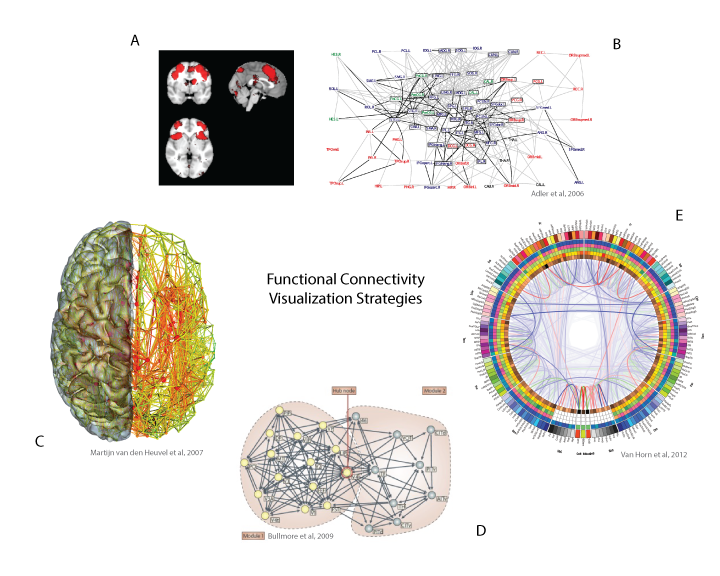
\includegraphics[width=10cm]{images/figure62.png}
\end{center}
\caption{ \label{fig:62} Functional connectivity visualizations:  Trends in functional connectivity visualizations have changed over time, including A) the orthogonal view, showing an axial, coronal, and sagittal slice of a functional map overlayed on an anatomical brain, B: graph based network approaches that model regions as nodes and links as hubs, C) equivalent networks in the context of brain space, D) force directed graphs that represent connectivity with distance, and E) bundling techniques to group clusters of connections.
 \newline \newline}
\end{figure} 


\subsection{Integration of visualizations with technology and publication standards}
The sheer complexity of these datasets contrasts with the limitations of the amount of data that can be shown in a web browser, which is largely dependent on the memory of the machine accessing it.  Methods such as caching, edge computing, data replication, and proper utilization of database querying make the goal of showing some aspect of functional connectivity data a reasonable one.  In print media, the standard of publication is tied back to our preference to read books, and scientific journals themselves, which dates back to 1665 when Philosophical Transactions of the Royal Society was released as the first exclusively scientific journal.  The modern version of this trend is distribution of electronic articles, many of which are packaged nicely into PDF files.  Researchers typically export an image from a software tool, and then add additional labels or coloring in a vector graphics program.  This procedure is highly time intensive, and unfortunately, it is not a requirement to share the production procedure.  It would be highly valuable to have a web framework that not only standardizes the data processing, but also provides standards for visualization of the result.   

\section{Methods}
\subsection{Parcellation and connectivity matrix generation}
Functional imaging data was provided by the MyConnectome project (\href{http://www.myconnectome.org}{http://www.myconnectome.org}), for which all data, processing protocol, and code is publicly available through a standard data sharing agreement. For this prototype, a mean connectivity matrix from an individual was derived from all resting BOLD scans.  A parcellation procedure (\cite{Gordon2016-gn}) was used to define 565 distinct regions, each of which was used to mask the data to define timecourses.  Pearson correlation was used to generate the connectivity matrix, M, [565 x 565]. 

\subsection{Interface development}
\subsubsection{Web technology}
Data Driven Documents, ``D3'' is a JavaScript library based on web standards (HTML, SVG, and CSS) (\cite{Bostock2011-ei}) that allows for generation of interactive, web visualizations.  This technology was selected for development of this interface due to integration with multiple platforms and browser types, as well as the utilization of scalable vector graphics (SVG) to drive the visualization.  A SVG is a vector based graphic, meaning that it is well-suited for publication, and the graphic could be exported from the interface for this purpose. 

\subsubsection{Visualization Strategy}
The goals of the brain visualization were to provide a two-dimensional rendition of a brain that maintained anatomical spatial accuracy in its representation.  First, I created a matrix of parcel x,y,z coordinates, C (565 x 3) and calculated the Euclidean distances between coordinates, resulting in a distance matrix, Cd, of size (565 x 565).  I then used the cmdscale function in R (\cite{Cox1996-rd}) to transform the three dimensional matrix into two-dimensions.  MDS is a method for dimensionality reduction that can visualize any N dimensional dataset in fewer dimensions, allowing for projection of the three dimensional coordinates onto a two-dimensional plane.  The algorithm works by placing each of the three-dimensional points in such a way so that similarity between points is preserved in distances (\cite{Cox1996-rd}).  This resulted in a flat axial image of brain coordinates onto which connections can be mapped. 

\subsubsection{Data Filtering}
Portrayal of all 565 x 565 = 319,225 connectivity values in the matrix would generate a slow visualization, and so it was decided to threshold values to include the top 1\% of both positive and negative values using the ``quantile'' function in R (\cite{Hyndman1996-ho}) for a total of N=3,914.
  
\subsection{Design choices}
\subsubsection{Coloring, thickness, and size}
The parcels that form the two-dimensional brain mapping are each colored by the functional network to which they belong, and this coloring is consistent with a set of large buttons above the brain that the user can click to turn ``on'' or ``off'' a particular network.  The links are colored with a gradient, so in the case of a connection between parcels from different networks, the color transitions seamlessly.  The node size changes dynamically to reflect the number of connections to it, and the viewer can click on nodes to highlight connections.

\subsubsection{Dimensionality}
The next challenge was orienting the viewer in a three-dimensional space with a two-dimensional image.  A simple strategy was utilized that, upon moving the cursor over any particular parcel on the brain map, shows the viewer an axial orthogonal slice with a bright red spot to indicate the parcel location.

\subsubsection{Data Values}
An interface cluttered with data values can distract the viewer, and so ``tooltips,'' or boxes of information that appear upon moving the cursor over an object in the visualization, were utilized to give feedback on links strengths, and node x,y,z coordinates. 

\subsubsection{Interface Controls}
The main control panel, including buttons to turn links associated with networks ``on'' or ``off'' and a slider to threshold the connectivity value, is placed above the brain map for easy accessibility.  Dynamically changing summary statistics (mean, min, max, counts) are on the left panel.  The right panel includes image export options.  The finished prototype is available at \href{http://vsoch.github.io/mybrain}{http://vsoch.github.io/mybrain}.

\section{Discussion}
The MyBrain prototype is a novel, two-dimensional interface that would allow for easy exploration and rendering of a functional connectivity matrix in context of the regions and functional networks that are of particular interest to the researcher.  While the short term goal of this prototype was to allow for critical thinking about the challenges and goals of visualization of this data, the larger goal is to develop a tool for a researcher to use for his or her data.  Ideally, the neuroimaging community will have a package or application program interface (API) with functions to easily generate custom, interactive web visualizations.  The ideal would be to integrate these visualizations into a web-based tool with a server backend that can allow a researcher to securely log in, upload raw datasets, and have the datasets processed in a standard way. The researcher could share links or directly embed elements of the visualization in a blog post, publication, or simply take static screen shots of a particular finding he or she has discovered when exploring the data.  

\section{Conclusions}
I have developed a web interface prototype that allows for visualization and exploration of functional brain connectivity data.  The interface is simple, intuitive, and allows for exporting of data to a format that would be extendable to a publication figure.  Tools of this nature are essential during a time when visualization is so important for comprehending meaning from inherently complex data.  This author is excited for what is to come in the next decade to better empower researchers to share and communicate their hard work.

\chapter{Best Practices for Reproducible Research}

An often overlooked component in the development of methods and data
standards, essential to their ultimate impact, is implementation to
ensure broader use and reproducibility. Toward this goal, I discuss best
practices for conducting reproducible research, with an emphasis on
infrastructure (Specific Aim \#4, Section 1.6). To supplement these
examples, I describe novel web-based tools and visualization strategies
I have developed over my graduate career. In this chapter, I stress the
emerging need for improved software development practices in academia. I
review the technology and frameworks that are necessary to produce
web-based tools that can be used for better standardization,
visualization, and ultimately reproducible science. I highlight the
challenges, strengths, and what I have learned from software developed
during my academic career that strives to meet these goals.

\section{The Reproducibility Crisis}

Making inferences from image comparisons requires much more than the
existence of ontologies and methods, it calls for the consistent
practice of reproducible research. As current media has suggested \cite{Baker_undated-bx,Open_Science_Collaboration2015-hb,Open_Science_Collaboration2012-zr},
the reproducibility of neuroimaging and cognitive science is messy at
best. Reproducibility goes far beyond the creation of a single database
to deposit results, and factors such as careful documentation of
variables and methods \cite{Crook2013-fe,Chirigati2013-qw},
how the data were derived \cite{noauthor_2014-zc,Stodden2014-ca,Wandell2015-yt},
and dissemination of results \cite{Nichols2015-um,Stodden2014-ca} unify
to embody a pattern of sound research practices that have previously not
been emphasized. Any single step in an analysis pipeline that is not
properly documented, or does not allow for a continued life cycle of a
method or data, breaks reproducibility. In this reality, it is clear
that long term success in practicing reproducible science is asking much
more than domain expertise and publication from our researchers.

The neuroscience community was shamed in 2013 when it was suggested
 \cite{Button2013-ja} that studies in neuroscience were lacking statistical power, and failing the
most fundamental goal of science: to contribute evidence for a discovery
and replicate the result. While large-scale efforts are contributing
datasets of substantial size (\cite{Gorgolewski2015-gu,Van_Essen2013-fi}) to
allow for the critical assessment of findings in neuroscience, a much
more substantial problem is the habits and standards that are acceptable
for researchers to partake in from the initial generation of an idea
through the publishing of a completed manuscript. While a great burden
must be placed on the researchers to design sound experiments, conduct
proper statistical tests, and derive reasonable inferences from those
tests, many of the challenges of practicing reproducible science could
be resolved with the advent of better tools, meaning resources for
performing analysis, visualizing and capturing workflows, and assessing
the reproducibility of a result.

\subsection{The components of a reproducible analysis}

A reproducible analysis, in its truest definition, must be possible to
do again. This means several key components for the creation and life
cycle of the data and methods:

\begin{enumerate}
\item
  complete documentation of data derivation, analysis, and structure
\item
  machine accessible methods and data resources
\item
  automatic integration of data, methods, and standards 
\end{enumerate}

A basic first question is whether it is reasonable to asking for these
components from a neuroimaging research. The last few decades of
neuroimaging research have been primarily dominated by collection of
small datasets, and derivation of custom pipelines or manual processing
in graphical interfaces using a standard suite of software \cite{Liou2003-ue,Jenkinson2012-pr}.
Under these circumstances, it has been shown that results can vary based
on operating system \cite{Glatard2015-fn},
choice of analysis parameters and processing strategy, and the data
itself. The Stanford Center for Reproducible Neuroscience at Stanford
University \cite{noauthor_undated-it} founded
by Russ Poldrack in 2015 was a first step in addressing the disorganized
nature of neuroimaging analysis working on methods~and tools to instill
standards and best practices \cite{Gorgolewski2015-gu} into
the production of new results. The center aims to capture the
difficulties associated with the proper analysis of datasets by offering
reproducibility as a service. A truly reproducible analysis requires the
collection, processing, documentation, standardization, and sound
evaluation of a well-scoped hypothesis using large data and openly
available methods. From an infrastructural standpoint this extends far
beyond requiring expertise in a domain science and writing skills,
calling for prowess in high performance computing, programming, database
and data structure generation and management, and web development. ~It
may not be feasible to expect an already heavily burdened academic
researcher to provide consistently standardized, well-documented, and
machine accessible products with varying and potentially limited
resources of a university. Further, the limited time of four to five
years of graduate training is not substantial to train both biological
domain and informatics experts. Thus, the center offers a novel
framework to take on this burden and offer reproducible analyses as a
service. Such a service would allows for the scientist to focus on the
sound acquisition of data, and on his or her expertise in asking the
original biological question. Under such a framework, the list of best
practices for reproducibility can not only be a suggestion, but an
implemented, standardized reality.

\subsection{Documentation}

While an infrastructure that manages data organization and analysis will
immediately provide documentation for workflow, this same standard must
trickle into the routine of the average neuroimaging scientist before
and during the collection of the input data. The research process is not
an algorithm, but rather a set of cultural and personal customs that
starts from the generation of new ideas, and encompasses preferences and
style in reading papers and taking notes, and even personal reflection.
~Young scientists learn through personal experience and immersion in
highly productive labs with more experienced scientists to advise their
learning. A lab at a prestigious University is like a business that
exists only by way of having some success with producing research
products, and so the underlying assumption is that the scientists in
training should follow suit. The unfortunate reality is that the highly
competitive nature of obtaining positions in research means that the
composition of a lab tends to weigh heavily in individuals early in
their research careers, with a prime focus on procuring funding for
grants to publish significant results. Thus, it tends to be the case
that young scientists know that it's important to read papers, take
notes, and immerse themselves in their passion, but their method of
doing this is unguided. In this scenario, a reasonable solution is not
to place higher expectation on the already encumbered scientists, but to
provide them with tools for learning and documentation.

\subsubsection{Documentation of Code}

In computational fields, it is typically the case that the most direct
link to reproducing an analysis is not perusing through research prose,
but by way of obtaining the code. Writing is just idea and hope until
someone has programmed something. Thus, a researcher in a computational
field will find it very hard to be successful if he or she is not
comfortable with version control \cite{Zandstra2013-st}.
Version control keeps a record of all changes through the life cycle of
a project. It allows for the tagging of points in time to different
versions of a piece of software, and going back in time. These elements
are essential for reproducible science practices that are based on
sharing of methods and robust documentation of a research process. It
takes very little effort for a researcher to create an account with a
version control service (for example,
\href{http://www.github.com}{http://www.github.com}),
and typically the biggest barriers to this practice are cultural. A
researcher striving to publish novel ideas and methods is naturally
going to be concerned over sharing ideas and methods until they have
been given credit for them. This calls for a change not only in
infrastructure, but research culture, and there is likely no way to do
that other than by slow change of incentives with example over time. It
should be natural for a researcher, when starting a new project, to
immediately create a repository to organize its life-cycle.~While we
cannot be certain that services like Github, Bitbucket, and Sourceforge
are completely reliable and will exist into infinitum, this basic step
can minimally ensure that work is not lost to a suddenly dead
hard-drive, and methods reported in the text of a manuscript can be
immediately found in the language that produced the result. Researchers
have much to gain in using these services. If a computational graduate
student is not using and established in using Github by the end of his
or her career, this is a failure in his or her training as a
reproducible scientist.

On the level of documentation in the code itself, this is often a
personal, stylistic process that varies by field. An individual in the
field of computer science is more likely to have training in algorithms
and proper use of data structures and advanced programming ideas, and is
more likely to produce computationally efficient applications based on
bringing together a cohesive set of functions and objects. We might say
this kind of research scientist, by way of choosing to study computer
science to begin with, might be more driven to develop tools and
applications, and unfortunately for academia will ultimately be most
rewarded for pursuing a job in industry. This lack of ``academic
software developers'' is another problem that I address later (Section
5.2), as it is arguably the prime reason that better, domain-specific,
tools do not exist for academic researchers. An epiphany that sometimes
takes years to realize is the idea that documentation of applications
lives in the code itself. The design, choice of variable names and data
structures, spacing of the lines and functions, and implementation
decisions can render a script easy to understand, or a mess of
characters that can only be understood by walking through each line in
an interactive console. Scientists in training, whether aiming to build
elegant tools or simple batch scripts, should be aware of these subtle
choices in the structure of their applications. Cryptic syntax and
non-intuitive processes can be made up for with a (sometimes seemingly)
excessive amount of commenting. Donald Knuth introduced the idea of
``literate programming,'' \cite{noauthor_undated-xh} a
methodology that includes both code and documentation in a single
document. Prime examples include iPython notebook, R-markdown, and
syntax highlighting in online material to combine code and text.
~Whether the researcher adds substantial comments, ~uses a literate
programming methodology, or communicates through variable naming and
flow of code, the goal is equivalent: to ensure that a researcher's flow
of thinking and process is sufficiently represented in his programming
outputs.

\subsubsection{Visual Documentation}

Documentation can be enhanced with better tools. For example, automated
documentation tools (e.g., Sphinx for python) \cite{noauthor_undated-sh} can
immediately transform comments hidden away in a Github repository into a
clean, user friendly website for reading about the functions.
~Scientists should be provided with these modern services because
arguably, dissemination of a result is just as important (if not more
important) than generation of the result itself. An overlooked component
toward understanding of a result is providing the learner with more than
a statistical metric reported in a manuscript, but a cohesive story to
put the result into terms that he or she can relate to. Visualization
accompanied with a story to connect the result to ideas that are easy to
synthesize can better distribute the result to both other researchers
and the larger community. For this reason, results cannot only live in
publications, but must be extended to visual documentation such as
websites, blogs, and media sources. What this means is that it might be
common practice to, along with a publication, write a blog post and link
to it. This process should be easier than it currently is, as not all
scientists know how to maintain a web presence. For example, a typical
poster presented at a conference might be easily transformed into
an~interactive, online poster. ~Static documents such as theses and
papers might immediately be parsed for sophisticated natural language
processing applications \cite{Feng_Niu_Ce_Zhang_Christopher_Re_Jude_Shavlik_undated-fp} to
be readily find-able by search engines, and more readily available for
social media discussion. A scientist should be immediately empowered to
publish a domain-specific web report that includes meaningful
visualization and prose for an analysis. Importantly, it must integrate
seamlessly into the methodology that it aims to explain, and associated
resources that were used to derive it. ~This desired functionality may
be beyond the scope of the academic researcher, and development of such
resources more suited for a new level of emerging scientist.

\section{The Academic Software Developer}

The need for reproducible science has brought with it the emerging niche
of the ``academic software developer,'' an individual that is a combined
research scientist and full stack software developer, and is well suited
to develop applications for specific domains of research. In this
section, I will discuss this interesting space that exists between
research and software development, along with the challenges of
developing software for reproducible science. As my expertise is in
neuroinformatics, I will provide example by way of tools that I've
developed for reproducible neuroimaging science. In Section 5.2.2, I
talk about pyneurovault, cogat-python, and the NIDM-api - all tools that
I have developed during my graduate career to deliver
neuroimaging-related databases directly into applications. I then give a
thorough overview of the modern technology required for developing tools
for reproducible research, including data structures, front and back-end
development, and high performance computing. In Section 5.3.5 I focus on
virtual machines, and a particular example of a reproducible workflow,
the MyConnectome Project. I then describe a set of web-based visualization tools that
represent the extension of my research into the applied space. In
Section 5.3.6, I discuss pybraincompare, a python module to immediately
deploy my semantic and spatial metrics for image comparison, and
visualize comparisons between pairwise maps. ~We start with a review of
modern infrastructure and data structures for developing these
applications.

\subsection{Machine Accessibility and Data Structures}

Resources for neuroimaging analysis should~be machine accessible, and
publicly available. While many services for documentation (e.g., Google
Docs), file storage (e.g., Amazon S3, Dropbox), and version control
(e.g., Github) offer seamless integration between a local machine and
the cloud, this does not guarantee that these resources are
programmatically accessible. While it may be possible to move files and
data by way of a command line, content such as free text in documents
and meta-data about files that is not captured in the researcher's
workflow is lost forever. ~The goal of making resources machine
accessible by way of standard data structures is highly challenging in
that there is a tradeoff between complexity and usability. A data
structure to describe a resource that is developed in a way to capture
every detail may be highly challenging to integrate into applications,
and turn developers away from using it. On the other hand, too simple a
data structure may fail to capture meaningful meta-data about the
resource(s) it intends to describe. Ideally, these standard data
structures should be intuitive, easy to use, and modern. In this
section, I will provide examples of machine accessible resources that
vary in the degree to which this goal is met.

\subsection{Application Programming Interfaces for Neuroimaging Research}

The previously discussed NeuroVault database for obtaining whole-brain
statistical maps, or the Cognitive Atlas for providing a description of
cognitive neuroscience, are not useful in applications if they existed
only as websites. Machine accessibility usually comes by way of an API,
or an application programming interface. Further, this API must be
developed to provide a data structure that encourages its use in the
development of applications for research because it is intuitive, easy,
and modern. One of my first goals in my early graduate career was to
develop these APIs for the databases and web resources that I knew were
important for distribution to the larger public.

\subsubsection{pyneurovault}

The first step to developing an API is considering the two domains that
are being connected. Neuroimaging science is moving heavily toward the
use of Python, or ``pythonic'' tools, and so it is a logical decision
that the NeuroVault database uses the Django
(\href{http://www.djangoproject.org}{http://www.djangoproject.org})
framework as a back-end, as it is a python framework and will allow for
seamless integration of these tools into the functions of the database.
This initial step can be seen as a strategy to integrate the tools that
neuroimaging scientists are developing into the larger framework of the
web. The next question is how to properly distribute the NeuroVault
database as a repository of brain maps, and for this I have developed a
two-pronged strategy. First, NeuroVault must be able to provide both
researcher and other web applications with access to metadata about
images, and file locations to download images. Toward this goal, it was
decided to provide a RESTful (representational state transfer) API
\cite{Pautasso2014-lr}, which means using hypertext transfer protocol (HTTP) or urls to send
(POST) and retrieve (GET) data. What this means is that NeuroVault
provides a set of formatted URLs
(\href{http://neurovault.org/api-docs}{http://neurovault.org/api-docs})
that users can use to query the database, and retrieve results in the
JSON (JavaScript Object Notation) format. For a researcher who is
comfortable with using different APIs, it is common knowledge that these
kind of APIs can integrate seamlessly into analysis pipelines in almost
any language simply by retrieving the web page, and parsing the JSON
object into a data structure that is familiar to the language and
researcher. Other web applications, by default of the domination of
JavaScript over the internet, would be able to easily integrate this
resource a well. As an additional step, due to the fact that a large
portion of neuroimaging researchers are comfortable working in python, I
developed pyneurovault (https://github.com/NeuroVault/pyneurovault), a
python wrapper for this RESTful API so that functions are designed to
form the RESTful queries, and convert filtering and specification of
various parameters into easy to use functions in python.

\subsubsection{cogat-python}

The Cognitive Atlas, by way of being an older database, includes a more
standard RESTful API based on a third-party language converting SQL
commands to the relational database to output the equivalent JSON data
structures. I developed an equivalent python wrapped, cogat-python
(cogat-python.readthedocs.org) to immediately empower neuroimaging
scientists most comfortable with python to query the concepts, tasks,
and contrasts in the atlas. This API was released early 2015, and has
been the driver behind the body of work presented in this thesis.
Interestingly, before the development of the RESTful API and python
wrapper, the Cognitive Atlas was equipped with a form of semantic
technology for users and developers. This technology, discussed in the
next section, provides a clear example for how a web resource must be
matched to its users and easily integratable into analysis frameworks,
otherwise it will not be used.

\subsubsection{expfactory-analysis}

Akin to NeuroVault and the Cognitive Atlas, the Experiment Factory
Docker infrastructure is a web interface that holds behind it a mine of
behavioral data. An additional challenge in this case is the fact that
this data might contain identifying information about participants that
participated in a battery on Amazon Mechanical Turk, and should not be
publicly available. To address this concern and still provide a RESTful
API to serve results programatically, the application allows users with
an account to generate tokens that can be embedded in the request from
any application to use it. To make this process easy, I developed a
Python wrapper to the Experiment Factory RESTful API
(expfactory-analysis, available at
\href{https://github.com/expfactory/expfactory-analysis}{https://github.com/expfactory/expfactory-analysis}) that, in one line,
will retrieve paginated results given an acceptable token:

from expanalysis.api import get\_results

access\_token = ``abcdefghijklmnopqrstuvwxyz''

results = get\_results(access\_token=access\_token)

While security and protection of personal health information (PHI) is
outside the scope of this review, it is an essential detail to many
sources of data, and care should be taken to ensure protection of
private data when generating data structures and tools to query them.

\subsection{The Vision of the Semantic Web}
The semantic web is a set of standards released by the World Wide Web
consortium for data structures and standards \cite{noauthor_undated-by} that
can be used to turn the internet into a web of data, instead of a web of
documents. The basic data structure that defines this standard is the
Resource Description Framework (RDF), which can be thought of as a text
file that defines resources, and then describes how they relate to one
another, typically with the format of:

resource1 --> relationship --> resource2

These relationships, called ``RDF triples'' form the basis of a graph.
The vision of the semantic web is a beautiful one \cite{noauthor_undated-by}:

\textit{The overall vision of the Data Activity is that people and organizations
should be able to share data as far as possible using their existing
tools and working practices but in a way that enables others to derive
and add value, and to utilize it in ways that suit them. Achieving that
requires a focus not just on the interoperability of data but of
communities.}

Unfortunately, there is a wide gap between the developers of this
standard, and its application. RDF is an example of a data structure
that has a steep learning curve for use, and requires substantial effort
by semantic web folk to make its contents readily accessible to standard
web developers. The main language to parse these documents, ``sparql'' \cite{noauthor_undated-hy},
does not bring with it an intuitive understanding and easy of use that
is prevalent in a language like python. While it could be that this
vision is sound and simply more work is needed to refine the standard,
this author believes that the standard is not being more integrated into
web applications because it's just too hard. These standards are
struggling not due to a lack of time and care put into developing them,
but because they do not easily extend to easy integration into the
workflows and practices that modern developers are accustomed to. ~As a
web developer, or a researcher that heavily uses Python, the first
thought that comes to mind when being exposed to a new data structure
should not be ``How do I get it out of this format?'' ~This is an
unfortunate reality, and a risky pursuit to push such a data structure
that stands in sheer opposition to the way that people naturally think
about modeling the world.

\subsubsection{The Neuroimaging Data Model (NIDM)}

An example of a set of models that use RDF as data structures in
neuroimaging is the The Neuroimaging Data Model (NIDM) \cite{noauthor_undated-pr}.
NIDM~is an extension of some of the World Wide Web consortium's models
to describe the outputs of neuroimaging analyses, including Results,
Experiments, and Workflows. The vision of the NIDM working group is
strong in that the standard aims to~define a standard data structure to
export the output of an analysis, and extend to other applications.
Recognizing this importance and the difficulty of using RDF, I devoted a
portion of my graduate career to the development of web-based tools for
neuroimaging scientists that integrates these data structures.

\subsubsection{The NIDM-Viewer}

The object model called ``NIDM-Result'' is a data structure produced
from analysis software that describes the parameters used in derivation
of a statistical brain map result. ~For example, an NIDM data structure
that goes along with a statistical brain map would describe peak
coordinates, their values, processing choices to describe the maps, and
links to all other related maps. This information would be useful to
integrate into a web application, but tools to parse the information
from RDF itself and deliver the information in a web interface had not
been developed.

Using the NIDM Results data structure, my first effort was to develop an
NIDM-Viewer than can immediately visualize brain maps and associated
significant coordinates in a web browser. I created the NIDM-Viewer
(\href{http://vsoch.github.io/nidmviewer}{http://vsoch.github.io/nidmviewer}),
which can be run from a local machine or on a server to visualize and
browse the result of a neuroimaging analysis. The back-end technology to
produce this output was a Flask (Python) application, meaning that the
Python modules could also be integrated into pythonic tools (e.g.,
Django). Thus, a logical next step was integration of this viewer into
the NeuroVault database (implemented in Django) so that researchers
sharing NIDM-Results can immediately and interactively browse these
results without needing to know the Sparql query language or interact
with the data structure (Figure~\ref{fig:51}).

\begin{figure}[ht!]
\begin{center}
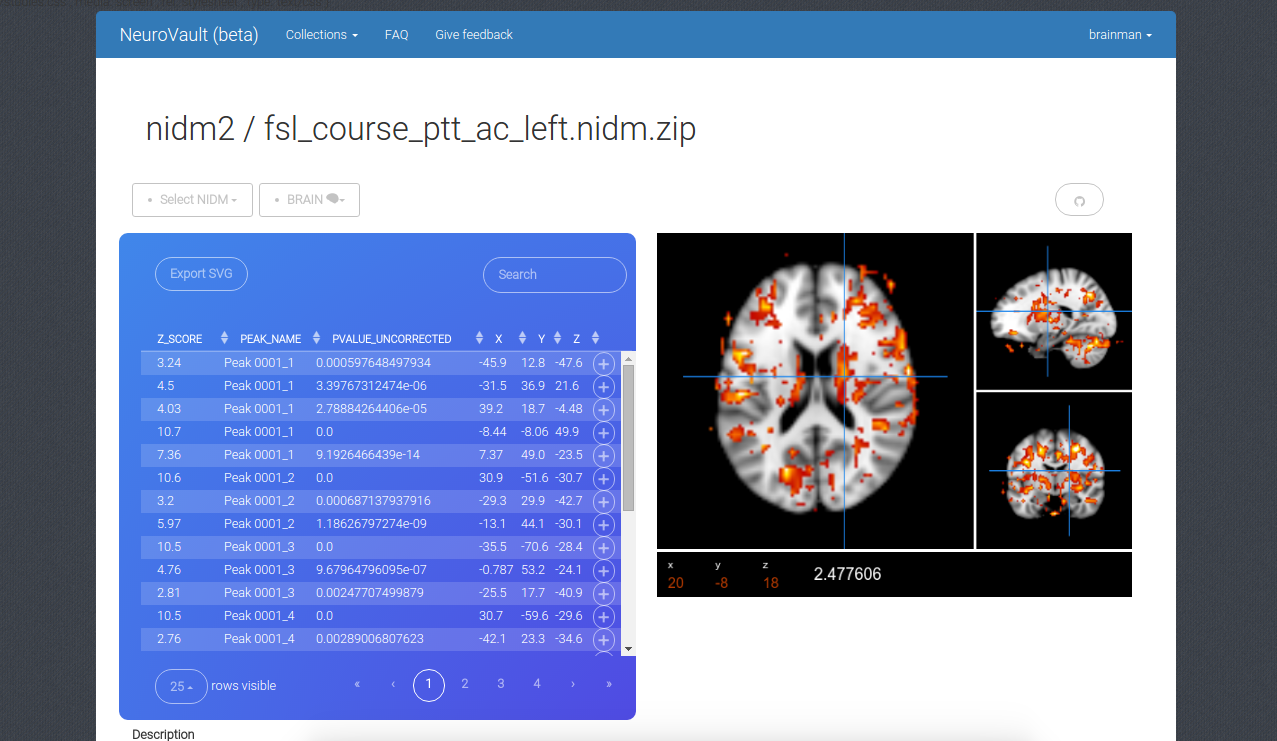
\includegraphics[width=15cm]{images/figure51.png}
\end{center}
 \textbf{\label{fig:51} Figure 5.1 }{ The NIDM Viewer used Python to parse three dimensional brain
coordinates and statistical result values from locations in the brain
map into an interactive table alongside the brain map itself.
}
\end{figure}

This is an example of distributing an easy to use tool that immediately
empowers a neuroimaging researcher to compare his or her result to
others, as the viewer can render any set of NIDM-Results files that are
available to it.

\subsubsection{The NIDM-api}

While the NIDM-Viewer initially worked by way of embedding sparql
queries into the application itself, this workflow was extremely
challenging from a development standpoint. The core issue was that
integration of Sparql queries into a browser, to query RDF and generate
a web-friendly data structure (JSON), was not standardized. The workflow
that was required to generate the viewer, specifically having expertise
to write Sparql queries and run them in Python, would never be tolerated
or even possible for a standard web developer. I had the insight that
the proper way to address this informatics problem would be to serve the
queries in a format that is tolerable and easy. My solution was to
develop an open source framework that would separate serve the results
of Sparql queries by way of a RESTful API
(\href{http://nidm-api.readthedocs.org}{http://nidm-api.readthedocs.org})
using a python web framework
(\cite{noauthor_undated-ia}),
the NIDM-api. The second insight was that the queries themselves should
be served in an intuitive data structure (JSON), and maintained
separately from the software to serve them to allow for specialization
of expertise. The NIDM-api (manuscript under review) can dually provide
a tool to serve Sparql queries against RDF documents, and interactive
web interfaces for generating new query objects and visualizing results.

The logic behind this application is that the software cleanly separates
the the queries themselves from the application serving them by way of
different Github repositories. Upon starting the application, the most
recent set of queries is programatically obtained from Github, and
served to the user both in interactive web interfaces and by way of a
RESTful API. The query repository can be maintained by the experts in
the semantic web, and the framework to serve them by developers that may
not have expertise with sparql or RDF. Individuals with expertise in
Sparql but possibly not programming skills can generate and interact
with queries via an interactive web interface (Figure~\ref{fig:52}) and
developers with no expertise in sparql that want to perform queries
don't have to see or know that it exists. ~

\begin{figure}[ht!]
\begin{center}
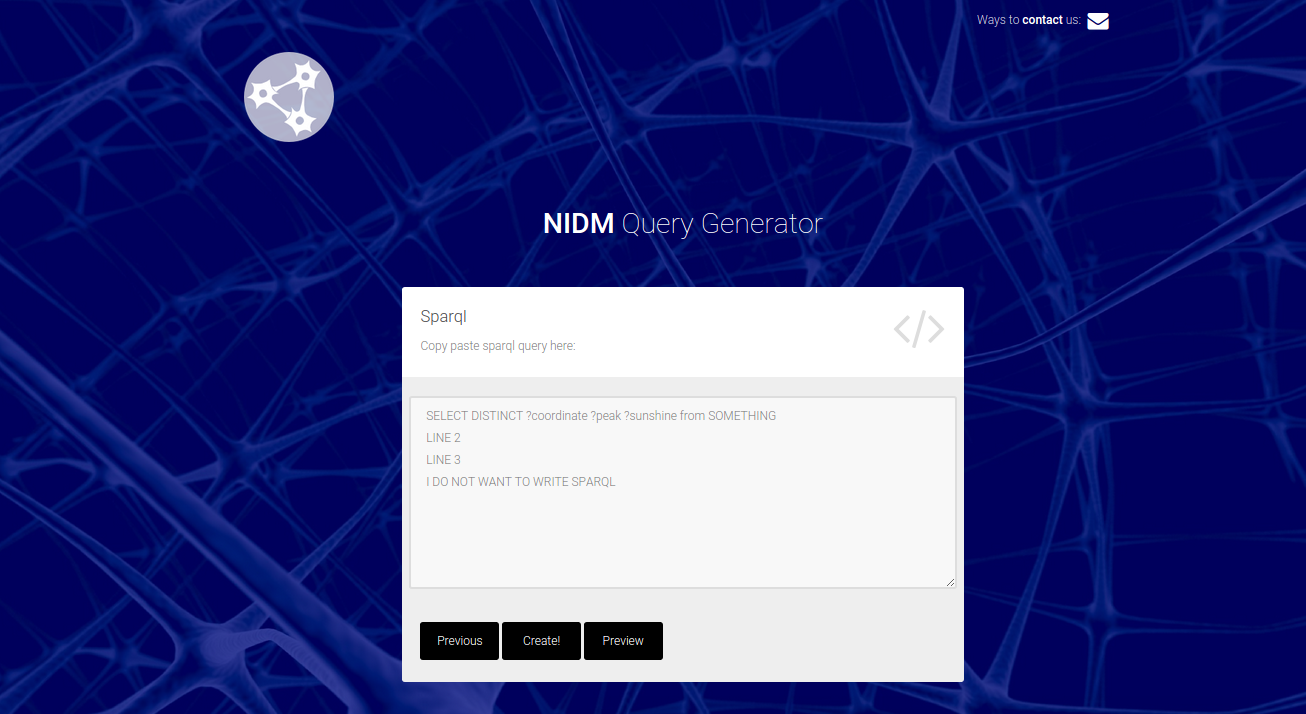
\includegraphics[width=15cm]{images/figure52.png}
\end{center}
 \textbf{\label{fig:52} Figure 5.2 }{ The NIDM-api includes an interactive web interface to
generate query data structures to serve in the Github repo for queries,
nidm-query.}
\end{figure}

This ensures that, if a software developer outside of the NIDM group
wants to develop an application that makes inferences over these data
structures, he or she will not have to know or understand Sparql or RDF
to do so. For academic software developers, the lesson to be learned is
to develop for the now, not for the idealized future.

\subsection{Frontend and Backend Web Frameworks}

The development of tools for researchers, along with visualization of
documentation and results, requires both expertise for writing code on
web or server for analysis (a ``back-end'') or code that is rendered
directly in a web browser for the user (``front-end''). Thus, an
academic software developer must have expertise in both these domains.

\subsubsection{Back End Frameworks}

The back-end framework refers to the organization and choice of
databases, machines, and any operation that must be run on a server to
ensure the proper function of an application. These operations are
typically not ``seen'' by the user, and require design choices that take
into account the anticipated usage of the application, security and
redundancy, and the applications themselves \cite{Murty2008-xr}.
For example, when deploying a reproducible workflow, the MyConnectome
Project (Section 5.2.7), Elastic Load Balancing, a strategy to deploy an
application on several servers and direct incoming traffic to be
balanced over the servers, was needed to ensure consistent application
availability. ~Servers to host web applications must also make choices
about whether to server secure (SSL) connections. For example, the
Experiment Factory integrates with Amazon Mechanical Turk, and a
requirement for such an application is that it provides a sure (HTTPS)
connection. Such an application that will be used concurrently by many
users would also need a database optimized for this concurrency, such as
postgreSQL, ideally with encrypted data transfer between the application
and database. To achieve this, it was necessary to serve the encrypted
connection (typically on port 443) by way of authenticating the server
with SSL certificates. This means that any user browser navigating to
the page has assurance that the connection is encrypted, and any data
transfer is protected.

The core of web-based applications includes several back-end components.
Servers that are accessible on the internet have been assigned to it an
IP (internet protocol) address that can be found by other machines, and
have a web server open (typically at port 80 or port 443 for secure
connections) with permission to allow incoming traffic. A typical
application carries with it data, and so a relational database \cite{Smith2010-il,DuBois2008-vl} is
the bread and butter of modern data storage, and in some cases external
e services \cite{Murty2008-xr,Wheeler2015-nv} are
appropriate for retrieval of static files. There are various choices for
web servers \cite{noauthor_undated-rk},
as there are machines and hosts \cite{noauthor_undated-yg},
and a developer looking to configure a machine typically makes his or
her choice based on price, availability of development tools \cite{noauthor_undated-rq},
and previous experience. The take home point is that the setup of the
back-end technology for any application or service must be done with
care and concern for the data being served, the users, and the longevity
and affordability of the application.

\paragraph{Application Frameworks}
The back end framework can be seen as a bassinet to give security and
stability to that which it is meant to take care of, the application
itself. An application framework refers to the libraries of functions
that perform operations on the data, and generate a result for the
frontend application, the part of the infrastructure that is ``seen'' by
the user. Choice of an application framework is incredibly important as
it can streamline development. For early applications, the standard was
to write custom php \cite{noauthor_undated-kz} functions
to work with a relational database and return queries to the front end.
These scripts developed into standardized content management systems
(CMS) that cleverly packaged base infrastructures and functions to work
with databases, giving developers the ability to write custom script
``plugins'' to extend use of the application. My earliest work in
graduate school
(\href{http://vbmis.com/bmi/noisecloud}{http://vbmis.com/bmi/noisecloud})
provided a database of spatial and temporal brain imaging features
associated with artifact in functional MRI accessible via an API by way
of a CMS called Wordpress \cite{noauthor_undated-gm}.
This framework~is estimated to encompass al most 60\% of all CMS, and
approximately a quarter of all websites on the internet \cite{noauthor_undated-gm}.
However, the lesson I learned from this early experience is that
Wordpress is a blogging platform, and not well suited for research
applications that require more than sharing of text and image content. I
realized quickly that Python-based \cite{noauthor_undated-ia,noauthor_undated-ej},
or server side JavaScript \cite{Foundation-jqueryorg_undated-ra} were
more modern, flexible choices, empowering the user to create more custom
user experiences. Early in my graduate school career, tools for easy
deployment of data analysis content was not properly developed, and
during this short time the statistics community that uses software
called R has made substantial progress to deliver these applications on
the web via a shiny server \cite{noauthor_undated-sj}.
Shiny~has become a popular avenue for data scientists to publish
interactive charts, however several issue remains. Hosting of such
applications is still limited \cite{noauthor_undated-gd} and
expensive, and the server itself not easy to set up. It would be highly
valued for a University or academic institution to provide hosting, or
minimally an avenue to serve these research-oriented applications. Shiny
is an example of just one framework, and an academic software developer
must be aware of and comfortable working with the most modern frameworks
that can easily transform data and scientific result into an interactive
web-based experience. Beyond expertise in setting up a server and coding
an application, this requires front-end expertise as well.

\subsubsection{Front End Resources}

The front-end framework refers to the library of functions and scripts
that define the user experience, which is typically text, images, and
interactive content rendered on a web page. The base of this content is
HTML5 \cite{noauthor_undated-ov},
which is not a language but a syntax that a browser understands how to
render to properly display content. The style of a page comes by way of
cascading style sheets (CSS3) \cite{noauthor_undated-qj},
and dynamic content most typically comes by way of JQuery \cite{Foundation-jqueryorg_undated-ra},
a javascript library that is used by over 60\% of the top 100,000
websites \cite{Foundation-jqueryorg_undated-jc}.
While the front-end design may seem less important than the application
itself, the user experience is an often overlooked essential component
in software design that can make or break the success of an application.
There are several resources for front-end developers that combine
components of front-end design \cite{Gandy_undated-mp,noauthor_undated-yt,Mark_Otto_Jacob_Thornton_and_Bootstrap_contributors_undated-is},
and during my time in graduate school I found myself devoting much time
to learning these frameworks to provide modern visualizations to
accompany my research.~I quickly found it obvious that these resources
were not developed specifically for research scientists, and attributed
the lack of equivalent resources for this purpose due to the inability
of the academic landscape to attract and keep experienced developers.
For example, there is a web font,~``font awesome,'' that provides
standard web icons that are hidden among most websites. There are no
statistical symbols or icons related to specific scientific domains
provided in this library, and as an early graduate student I saw no
reason that resources of this caliber could not exist for researchers.
During my graduate career I developed a web font, ``font-brain'' that
would provide meaningful symbols for neuroimaging scientists to embed
into web applications, manuscripts, or code repositories
(\href{https://vsoch.github.io/font-brain}{https://vsoch.github.io/font-brain}). While Font-brain's usage is limited to a
set of my applications, it is an example of how modern resources are
needed for brain imaging scientists.

\subsection{Development Architecture}

Development of applications requires many individuals working
collaboratively on a common code base. it requires careful, regular
testing of code (continuous integration), along with generation of a
consistent development environment for developers to ensure that server
architecture matches development architecture. In this section I will
cover standard routine for collaborating on a code base (version
control), along with development workflows and container-based
architectures.

\subsubsection{Continuous Integration}
As previously discussed, Github is an essential choice for software
developers to collaborate on coding projects in that it provides version
control. ~An application's code can live in a central repository (repo),
and the repository has different branches, or versions of the
application that are being actively developed. The repo typically has a
``master'' branch where the production quality application is stored,
and making changes to this branch is done by way of a ``pull request,''
(PR) which is a process of comparing a modified branch's code to the
master, and having a discussion about the changes. The PR is typically
set up to automatically perform ``continuous integration,'' or running a
series of tests over all of the proposed changes to make sure that no
functionality has been broken by the changes. Continuous integration
(CI) is provided to developers as a service \cite{noauthor_undated-nz,noauthor_undated-nm},
and can be used to test the application on different system setups, as
well as render application outputs that are static files. Writing good
tests is an art in itself, and another important step in developing
applications that aim to have longevity.

While the base case of CI is to test a code base, it should not go
unnoticed that such a service will allow for running a snippet of code
over any function of interest in a github repository. While not the
original intention, a service like continuous integration would allow
for a researcher to share code, and if another researcher copies (forks)
the repo, the code could be run immediately to produce an output. ~

\subsubsection{Container-based Architectures}

A modern description of web technology would not be complete without a
discussion of container-based architecture. Docker \cite{noauthor_2015-vu} has
emerged as a promising framework to streamline development for
reproducible research \cite{Boettiger2014-cz}.
and development workflows. Docker is based on the idea of creating
different ``containers'' for each component of an application, and a
container can encompass any single entity that can be installed on a
server. Containers can be shared \cite{noauthor_undated-xe} to
allow for reproducible workflows, and utilize a system's resources in a
more resourceful way than installation of the equivalent number of
virtual machines \cite{Vaughan-Nichols2015-sg}.
Developing an application with Docker means that it can easily be
deployed anywhere with root permissions \cite{noauthor_undated-lf},
and while this does not extend well to servers or high performance
computing (HPC) environments where this is not possible, it is a step in
the right direction to reproducible systems, and an improvement over
previous methods \cite{noauthor_undated-im}.

\subsection{High Performance Computing}

A major challenge to developing applications for science is the need for
high performance computing (HPC) \cite{noauthor_undated-tu}.
HPC is the use of massive grids of machines, connected together with a
job management system \cite{noauthor_undated-qg,noauthor_undated-yd} to
run jobs that require high computational resource such a memory or
storage in parallel. Most major universities give researchers access to
a grid of these machines, called a ``cluster,'' whether for free or for
a price. HPC can render an analysis that would take 8 months to run in
serial done within an hour in a parallel environment. The biggest
challenge for researchers is not using HPC, but rather, extending HPC to
work in a cloud environment \cite{Eadline_undated-rs},
integrated into a web application. This is a burgeoning area of
development with much promise \cite{noauthor_undated-sd}.
Further, the HPC environment is not yet friendly to container-based
architectures that can extremely improve reproducibility, discussed
next.

\subsection{Virtual Machines}

The choice of a back and front-end web framework, as well as a strategy
for collaborative development and continuous integration says nothing
about application deployment. While use of a hosted web server seems
like the ideal solution to share an application, it may not be
appropriate for a research product such as an analysis pipeline.
Further, analysis pipelines are complex entities, often requiring the
use of multiple programming languages with different libraries, access
to large data, and memory. In this context, a reasonable solution, and
on par with a container architecture, would be to package a
configuration into a virtual machine (VM). Virtualbox \cite{noauthor_undated-id} is
a leader in virtual machine deployment software, with wrappers such as
Vagrant \cite{noauthor_undated-tk} allowing
for command line control of machines. These virtual machines can not
only deploy applications, they can also be used for development
environments. With Vagrant, a single file called a Vagrantfile is run to
bring up an entire virtual machine, and such a file can be shared easily
on a service like Github. A virtual machine can be generated and
deployed on a user's local machine, or straight to a cloud service like
Amazon Web Services (AWS). This kind of immediate packaging of an
analysis holds great promise for distributing reproducible workflows,
and during my time at Stanford I have worked on deploying several
reproducible workflows in this fashion. A noteable example is the
MyConnectome Virtual Machine
(\href{https://github.com/poldrack/myconnectome-vm}{https://github.com/poldrack/myconnectome-vm}),
which integrates genomic, metabolomic, behavioral, and brain imaging
data from multiple sources into an analysis that can be immediately
deployed to the cloud
(\href{http://results.myconnectome.org}{http://results.myconnectome.org})
or on a user's local machine (Figure~\ref{fig:53}).

\begin{figure}[ht!]
\begin{center}
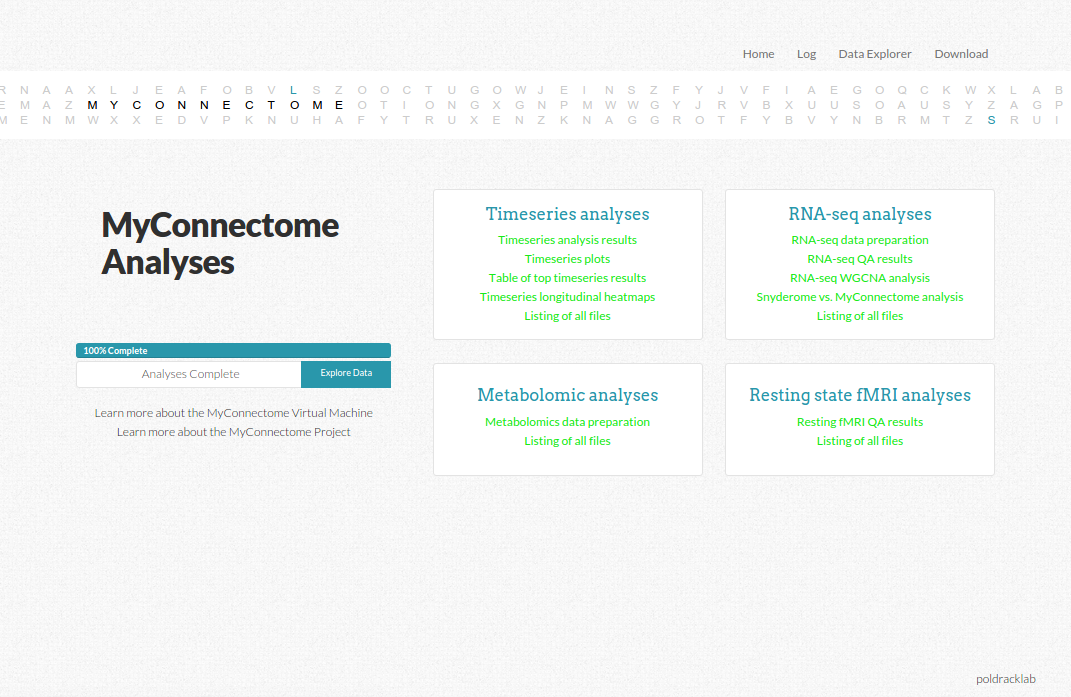
\includegraphics[width=15cm]{images/figure53.png}
\end{center}
 \caption{\label{fig:53} The MyConnectome virtual machine was a successful strategy
to completely reproduce a complicated analysis involving brain imaging,
genomics, behavior, and metabolomic data.}
\end{figure}

The core challenge was bringing together disparate data sources into one
computational environment, running complicated, time-intensive analysis,
and keeping the user updated about progress and errors. A solution was
needed to obtain data, process it, and render a result for the user. My
advisor Russell Poldrack approached me when he started developing this
pipeline, and challenged me to create an interface to integrate into a
virtual machine to interact with it. ~This task proved to be much more
challenging than anticipated. We quickly learned that the failure of a
single download would put a stop in the entire pipeline, which could
take upwards of 12 hours depending on internet connectivity, and it
would be required for the user to have command line expertise to ssh
into the virtual machine to debug or look for logs that might hint about
what went wrong. It was immediately clear that we needed some form of
communication of error and console output, and that the front-end user
interface must dynamically update as the back-end analyses are
completed. First, to make the generation of results on the virtual
machine transparent to the user, I linked all outputs to links on the
main interface, and these links would activate and change from gray to
green when the result was produced. To keep the user alert to the timing
of analyses, I generated logs of expected time based on results that
were generated, and wrote a function to reflect this timing in a
progress bar on the main interface. The lesson here is that there must
be accurate communication between a user and a tool, otherwise the tool
is not serving its purpose to reflect what is happening server side.

Finally, while many results were already web-friendly (e.g., ipython
notebook or R-markdown rendered into HTML), many results were tab
delimited files that were not. My goal was to use modern web technology
to render both results and output and error logs in a meaningful
fashion. Toward this goal, I created an interactive interface to render
error and output logs, and select result files from intuitively
organized drop down menus, and render in a sortable, clean table. The
final addition of a single download for all results completed the
virtual machine. The complexity of this project brought to light that
deploying a reproducible workflow, as a custom application, is
incredibly challenging, and must more care and thought must be put into
designing tools that make this process no more than the click of a
button.

\section{Web Based Tools for Neuroimaging}

We have reviewed the basic components of developing and deploying web
based tools. Technology for reproducible research means integration of
these components, including servers and databases, and high performance
computing, while keeping user experience and proper documentation in
mind to produce a final product that serves as the dissemination of the
result. In the modern age, a final product is typically expected to have
searching capabilities, intuitive design and visualization, and
integration with cloud resources.

\subsection{Visualization}

The sharing a result is almost impossible without showing something
meaningful. The reason for success of the internet as a platform for
reading, learning, and everything, is primarily because of the visual
experience that it affords. This means that, while it is often
undervalued, visualization is an important, if not one of the most
important, components for a web-based application. Data visualization
for highly dimensional and complex data can help to discover patterns,
generating hypothesis, and develop subsequent models of natural
phenomena. The task of rendering a single statistical brain map in a
browser, or a matrix of connectivity data \href{http://vsoch.github.io/mybrain/}{http://vsoch.github.io/mybrain/} is no simple thing. Modern javascript libraries such as D3 \cite{Bostock2011-ei} can
handle a few thousand objects in the browser before seeing huge
detriments to performance, and a queue technique using canvas \cite{noauthor_undated-hy} could
handle many more values, but renders them statically.

\subsubsection{Pybraincompare}

To unite the processing of brain images using python and web
visualization, I developed a python module, pybraincompare \cite{noauthor_undated-hu},
that works as a tool to perform some analysis of interest with a brain
image, and then immediately renders the result in the user's local
browser. The tool can generate web reports for quality analysis (QA),
scatterplots to compare two brain maps, connectograms, as well as tree
data structures to render ontological relationships (Figure~ref{fig:54}).

\begin{figure}[ht!]
\begin{center}
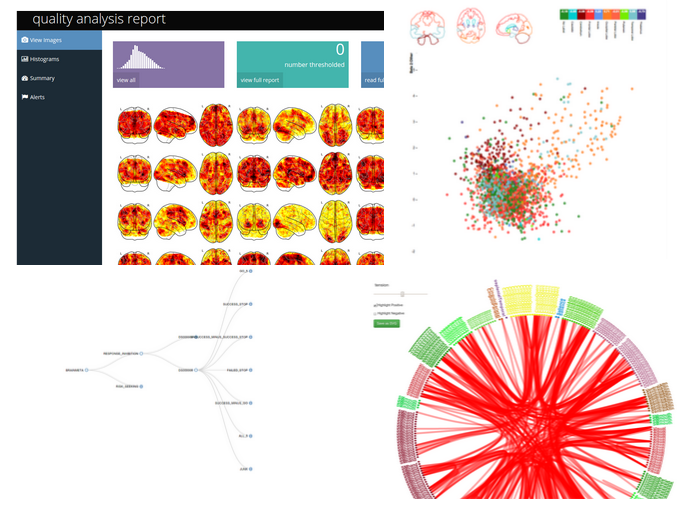
\includegraphics[width=15cm]{images/figure54.png}
\end{center}
 \textbf{\label{fig:54} Figure 5.4 }{ The Pybraincompare Python package produces several interactive visualizations for brain imaging analysis, including an interactive quality analysis report (top left), a scatterplot matrix to compare two images (top right), an ontology tree (bottom left), and a connectogram for functional MRI (bottom right).}
\end{figure}

Importantly, this python package also contains the spatial and semantic
methods that have driven the work of my thesis, allowing for a
neuroimaging researcher to deploy the same methods in his or her
pipelines. As an example, pybraincompare is the driver behind the
``image comparison'' feature in NeuroVault, taking responsibility for
both doing the computations, and rendering a search interface (Figure~\ref{fig:55}) as well as pairwise scatterplots to assess the similarity of two
images (Figure~\ref{fig:54} top right).

\begin{figure}[ht!]
\begin{center}
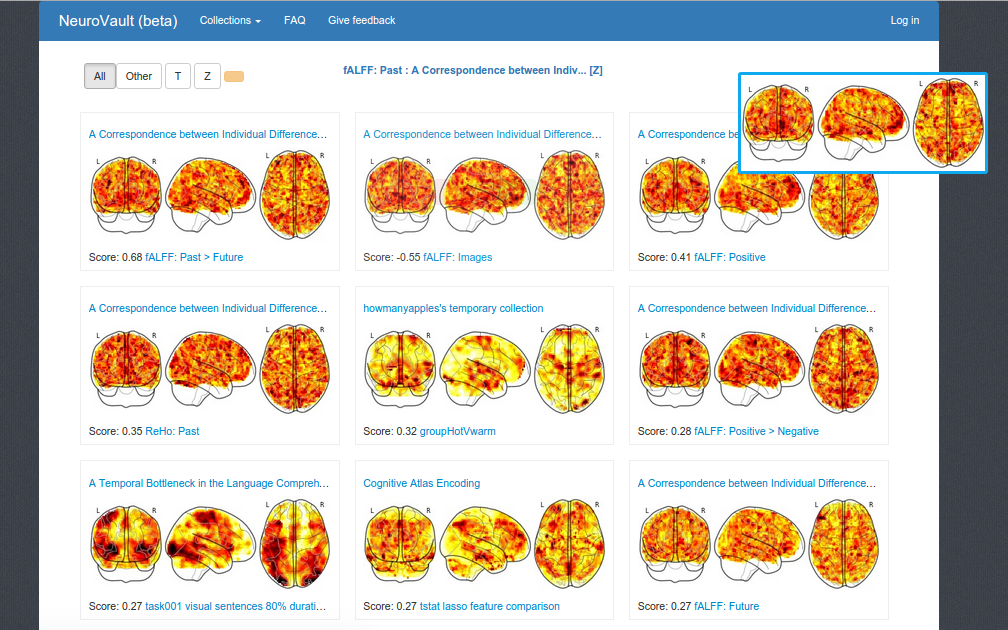
\includegraphics[width=15cm]{images/figure55.png}
\end{center}
 \caption{\label{fig:55} The Pybraincompare Python package renders the interactive search interface to power spatial image comparison in the NeuroVault database.}
\end{figure}

Pybraincompare also brings with it functions to generate output using
canvas, allowing for the rendering of over 150K data points in under 3
seconds. The contrast between a canvas rendering that allows for this number of data points and a D3 rendering that handles a few thousand demonstrates the trade-off between interactivity and usability. Generation of a visualization must be done in a
manner that is intuitive and transparent to the viewer, and the
visualization itself must strike a fine balance between revealing the
data's inherent complexity and providing an easily digestible
abstraction.

\subsubsection{Nifti-drop}

The drawback of a tool like pybraincompare is that it requires a server
or a local machine. As was previously noted, the divide between a user's
computer and the browser is getting fuzzy. Most user's of web
applications do not want to spend the time to download software, or even
go through extensive upload processes. This demand for instantaneous
function led me to ask the question if it would be possible to render a
complex data such as a brain image directly in a browser, and this
resulted in nifti-drop
(\href{http://vsoch.github.io/nifti-drop/}{http://vsoch.github.io/nifti-drop/}).
First, a nifti file is a standard data format in neuroimaging \cite{Mjenkinson2005-hk}.
It can store a 3D brain image, or a 4D brain image, meaning a 3D image
collected over time. The nifti-drop prototype uses modern web
technology, specifically the File Reader web API \cite{noauthor_undated-fz} to
allow for a user to drop one of these files directly on the browser, and
have the image data (the ``brain map'') and the header information (meta
data about the image) render immediately in the browser. The viewer also
supports dropping an NIDM-Results data structure (Section 4.3.1) to
immediately render the Contrast map and associated points. This project
uses JavaScript, HTML5, Bootstrap, along with the web query language
Sparql and FileReader, and putting all of these pieces together was
highly challenging.

\subsubsection{Brain Browser and Niindex}

As an extension to the nifti-drop, it seemed like a reasonable goal to
generate a small application to equivalently render a local brain map in
the browser, but allow for serving of images from the user file system.
Toward this goal, I developed the Brain Browser
(\href{https://www.npmjs.com/package/brain-browser}{https://www.npmjs.com/package/brain-browser}), a node-js application \cite{Foundation_undated-ud}.
It then became apparent that this kind of functionality might be desired
for a server, and so I modified the standard File Browser behavior of a
server to immediately render any brain images in a subset of folders, a
project that I called niindex
(\href{http://www.vbmis.com/bmi/project/niindex/}{http://www.vbmis.com/bmi/project/niindex/}). This string of brain viewers serves as an example for the kinds of ideas that can better fit
servers, local computers, and web sites to host highly complex brain
imaging data.

\section{A Future of Reproducible Science}

The focus of this final chapter has been on the technology and modern
practices for individual and organized reproducible research. I have
reviewed applications and virtual machines that I have developed to
exemplify how modern web and server technologies can be useful for
researchers. The next question pertains to how we can spur the
development of these domain-specific tools, or provide better resources
for researchers to practice reproducible science. It is clear that we
are in a decade of change, and the development of better services,
either provided by the university, or by an emerging new level of
``academic software developer,'' can help this reproducibility crisis.

If we have a vision for this kind of development, we must next determine
the right path for making that vision a reality. The standard now is for
university systems to provide high performance computing, some file
storage, and limited places for web sites or blogs for groups to
maintain an interface to the public. It could be the case that a
university establishes a university-wide resource for reproducible tool
development and training of researchers, or that the standard job-based
cluster resources are replaced with a container-based architecture that
could capture and deploy reproducible workflows. It could also be the
case that a better collaboration with industry, and providing research
as a service, could save academia. A simple overview of best practices
could be provided to new students, and staff in the center might come
from many flavors of science, and would devote their time to developing
domain-specific tools, or assisting researchers in extending findings
into tools that can be harnessed by others. Granting bodies might
prioritize establishing academic software developers across labs, and
this expertise would be provided on a local rather than university
level. ~While many continuous integration, version control, and hosting
services seem to offer long term products, the harsh reality is that
there really exists no insurance about any single web resource ``being
around forever.'' However, with sound research practices like creating
multiple copies (redundancy), assigning digital object identifiers
(DOIs), and creating proper documentation, we can maximize the longevity
and archiving of our results.


\bibliographystyle{plain}
\bibliography{thesis}
\end{document}